\documentclass[a4paper,12pt]{article}

% Основные пакеты
\usepackage[T1, T2A]{fontenc}
\usepackage[utf8]{inputenc}
\usepackage[english, russian]{babel}
\usepackage{geometry}
\usepackage{indentfirst}
\usepackage{graphicx}
\usepackage{wrapfig}
\usepackage{amsmath, amssymb, amsfonts}
\usepackage{braket} 
\usepackage{float}
\usepackage{amsmath}  % для математических окружений
\usepackage{bm}  
% Гиперссылки и цветовые настройки
\usepackage[dvipsnames]{xcolor}
\usepackage[colorlinks]{hyperref}
\hypersetup{
	linkcolor=blue,
	filecolor=magenta,
	urlcolor=cyan
}

\usepackage{listings}
\usepackage{xcolor}

% Цвета
\definecolor{backcolour}{rgb}{0.95,0.95,0.92}
\definecolor{codegreen}{rgb}{0, 0.5, 0}
\definecolor{codegray}{rgb}{0.4, 0.4, 0.4}
\definecolor{codepurple}{rgb}{0.58, 0, 0.82}
\definecolor{keywordcolor}{rgb}{0.0, 0.2, 0.7}
\definecolor{stringcolor}{rgb}{0.6, 0, 0}
\definecolor{framecolor}{rgb}{0.7, 0.7, 0.7}

% Стиль для Mathematica
\lstdefinestyle{python}{
	language=python,
	backgroundcolor=\color{backcolour},
	basicstyle=\ttfamily\small,
	keywordstyle=\color{keywordcolor}\bfseries,
	commentstyle=\color{codegreen}\itshape,
	stringstyle=\color{stringcolor},
	numberstyle=\tiny\color{codegray},
	numbers=left,
	numbersep=5pt,
	breaklines=true,
	breakatwhitespace=false,
	showstringspaces=false,
	keepspaces=true,
	frame=single,
	rulecolor=\color{framecolor},
	frameround=tttt,
	captionpos=b,
	tabsize=2,
	xleftmargin=1em,
	xrightmargin=0.5em
}

% Установить стиль по умолчанию
\lstset{style=python}

% Путь к изображениям
\graphicspath{{./images/}}

% Геометрия страницы
\geometry{left=2cm, right=2cm, bottom=2cm, top=2cm}

\begin{document}
	\begin{titlepage}
		\centering
		\vspace*{1cm}
		
		{\large Министерство науки и высшего образования Российской Федерации}\\
		{\large ФЕДЕРАЛЬНОЕ ГОСУДАРСТВЕННОЕ АВТОНОМНОЕ ОБРАЗОВАТЕЛЬНОЕ УЧРЕЖДЕНИЕ ВЫСШЕГО ОБРАЗОВАНИЯ «НАЦИОНАЛЬНЫЙ ИССЛЕДОВАТЕЛЬСКИЙ УНИВЕРСИТЕТ ИТМО»}\\
		{\large (УНИВЕРСИТЕТ ИТМО)}\\
		
		\vspace{2cm}
		
		{\large Факультет «Систем управления и робототехники»}\\
		
		\vspace{3cm}
		
		\textbf{{\Huge ОТЧЕТ}\\
			{\Huge О ЛАБОРАТОРНОЙ РАБОТЕ №5}}\\
		
		\vspace{1cm}
		
		{\LARGE По дисциплине «Частотные методы»}\\
		{\LARGE на тему: «Связь непрерывного и дискретного»}\\
		
		\vspace{3cm}
		
		{\Large Студент:}\\
		Охрименко Ева
		
		\vspace{2cm}
		
		{\Large Преподаватели:}\\
		Догадин Егор Витальевич\\
		Пашенко Артем Витальевич\\
		
		\vspace{3cm}
		{\large г. Санкт-Петербург}\\
		{\large 2025}
		
	\end{titlepage}
	\newpage
	\tableofcontents
	\newpage
	
	\section{Задание. Непрерывное и дискретное преобразование Фурье.}
	
	Рассмотрю прямоугольную функцию $\Pi: \mathbb{R} \to \mathbb{R}$:
	\[
	\Pi(t) = 
	\begin{cases}
	1, & |t| \leq \frac{1}{2} \\
	0, & |t| > \frac{1}{2}
	\end{cases}
	\]
	
	Вычислю фурье-образ функции $\Pi(t)$:
	\[
	\hat{\Pi}(\nu) = \int_{-1/2}^{1/2} e^{-2\pi i \nu t} dt = \left. \frac{e^{-2\pi i \nu t}}{-2\pi i \nu} \right|_{-1/2}^{1/2} = \frac{e^{\pi i \nu} - e^{-\pi i \nu}}{2\pi i \nu} = \frac{\sin(\pi \nu)}{\pi \nu} = \text{sinc}(\nu)
	\]
	
	Также приведу графики $\Pi(t)$ и $\hat{\Pi}(\nu)$:
	
	\begin{figure}[h]
		\centering
		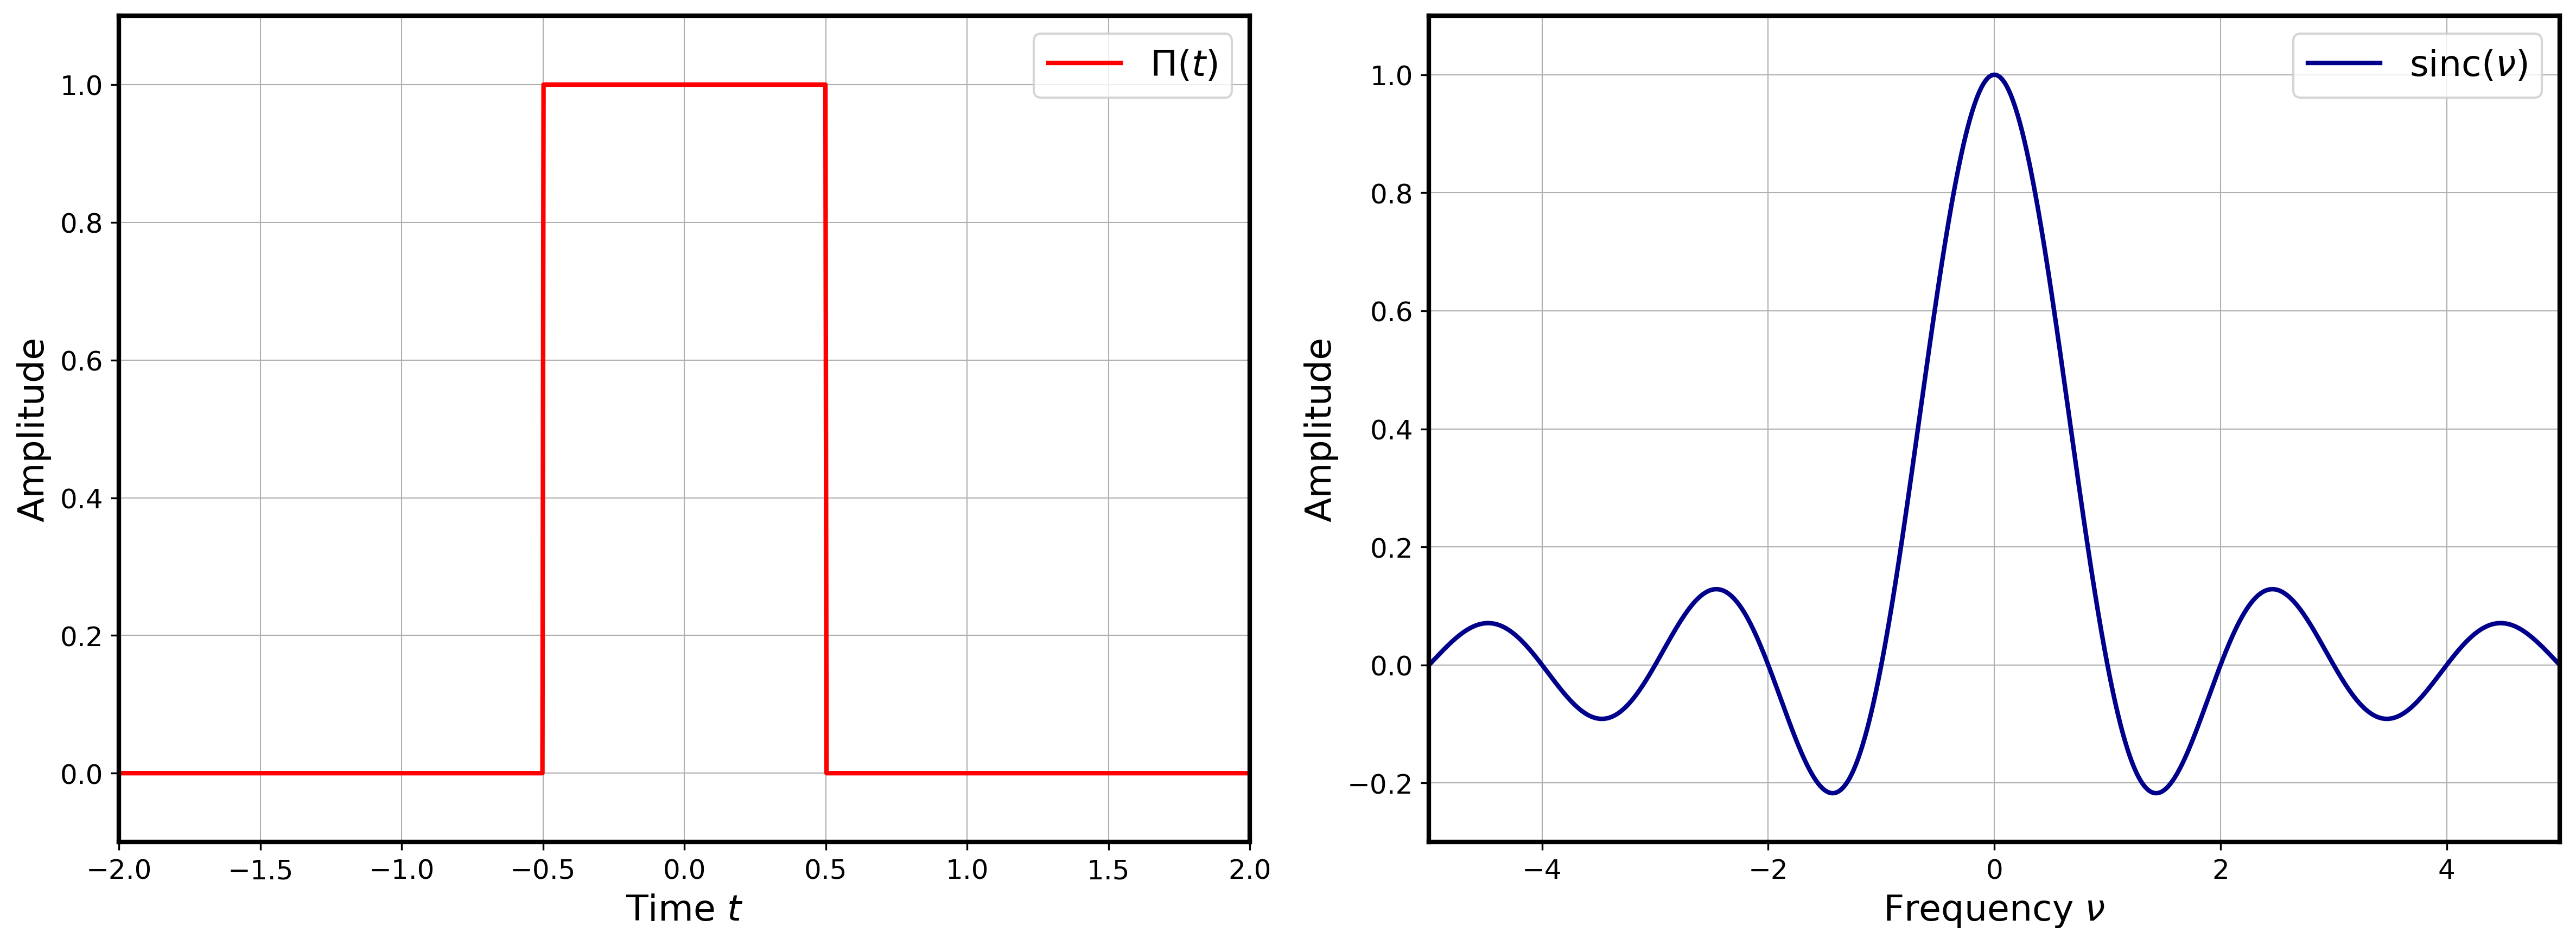
\includegraphics[width=1\textwidth]{../images/task1/first.png} 
		\caption{Графики функции и фурье-образа}
	\end{figure}

\newpage

\subsection{Численное интегрирование}\label{subsec:trapz}

В этом задании мне нужно задать функцию \(\Pi(t)\), найти ее Фурье-образ с помощью функции численного интегрирования \texttt{trapz}. Далее опять с помощью численного интегрирования выполнить обратное преобразование Фурье от найденного Фурье-образа, чтобы восстановить функцию. Мои схематичные действия: 

\[
\Pi(t) \xrightarrow{\text{trapz}} \hat{\Pi}(\nu) \xrightarrow{\text{trapz}} \Pi(t)
\]

\textbf{Ожидаемые результаты}

\begin{itemize}
	\item Наиболее показательные значения параметров $T$, $\Delta t$, $V$, $\Delta \nu$.
	
	\item Графики аналитического образа и найденного с помощью численного интегрирования $\hat{\Pi}(\nu)$.
	
	\item Графики исходной $\Pi(t)$ и восстановленных функций.
	
	\item Выводы о влиянии шага и промежутка интегрирования и о точности и быстродействии метода.
	
\end{itemize}
\hrule

\subsubsection{Предподготовка}

Задам функцию \(\Pi(t)\) в python. Зафиксирую параметры функции $T = 20$, $\Delta t = 0.005$, $V = 20$, $\Delta \nu = 0.005$. Отрисую полученные сигналы и образы, при этом засеку время вычислений. 

\begin{figure}[h]
	\centering
	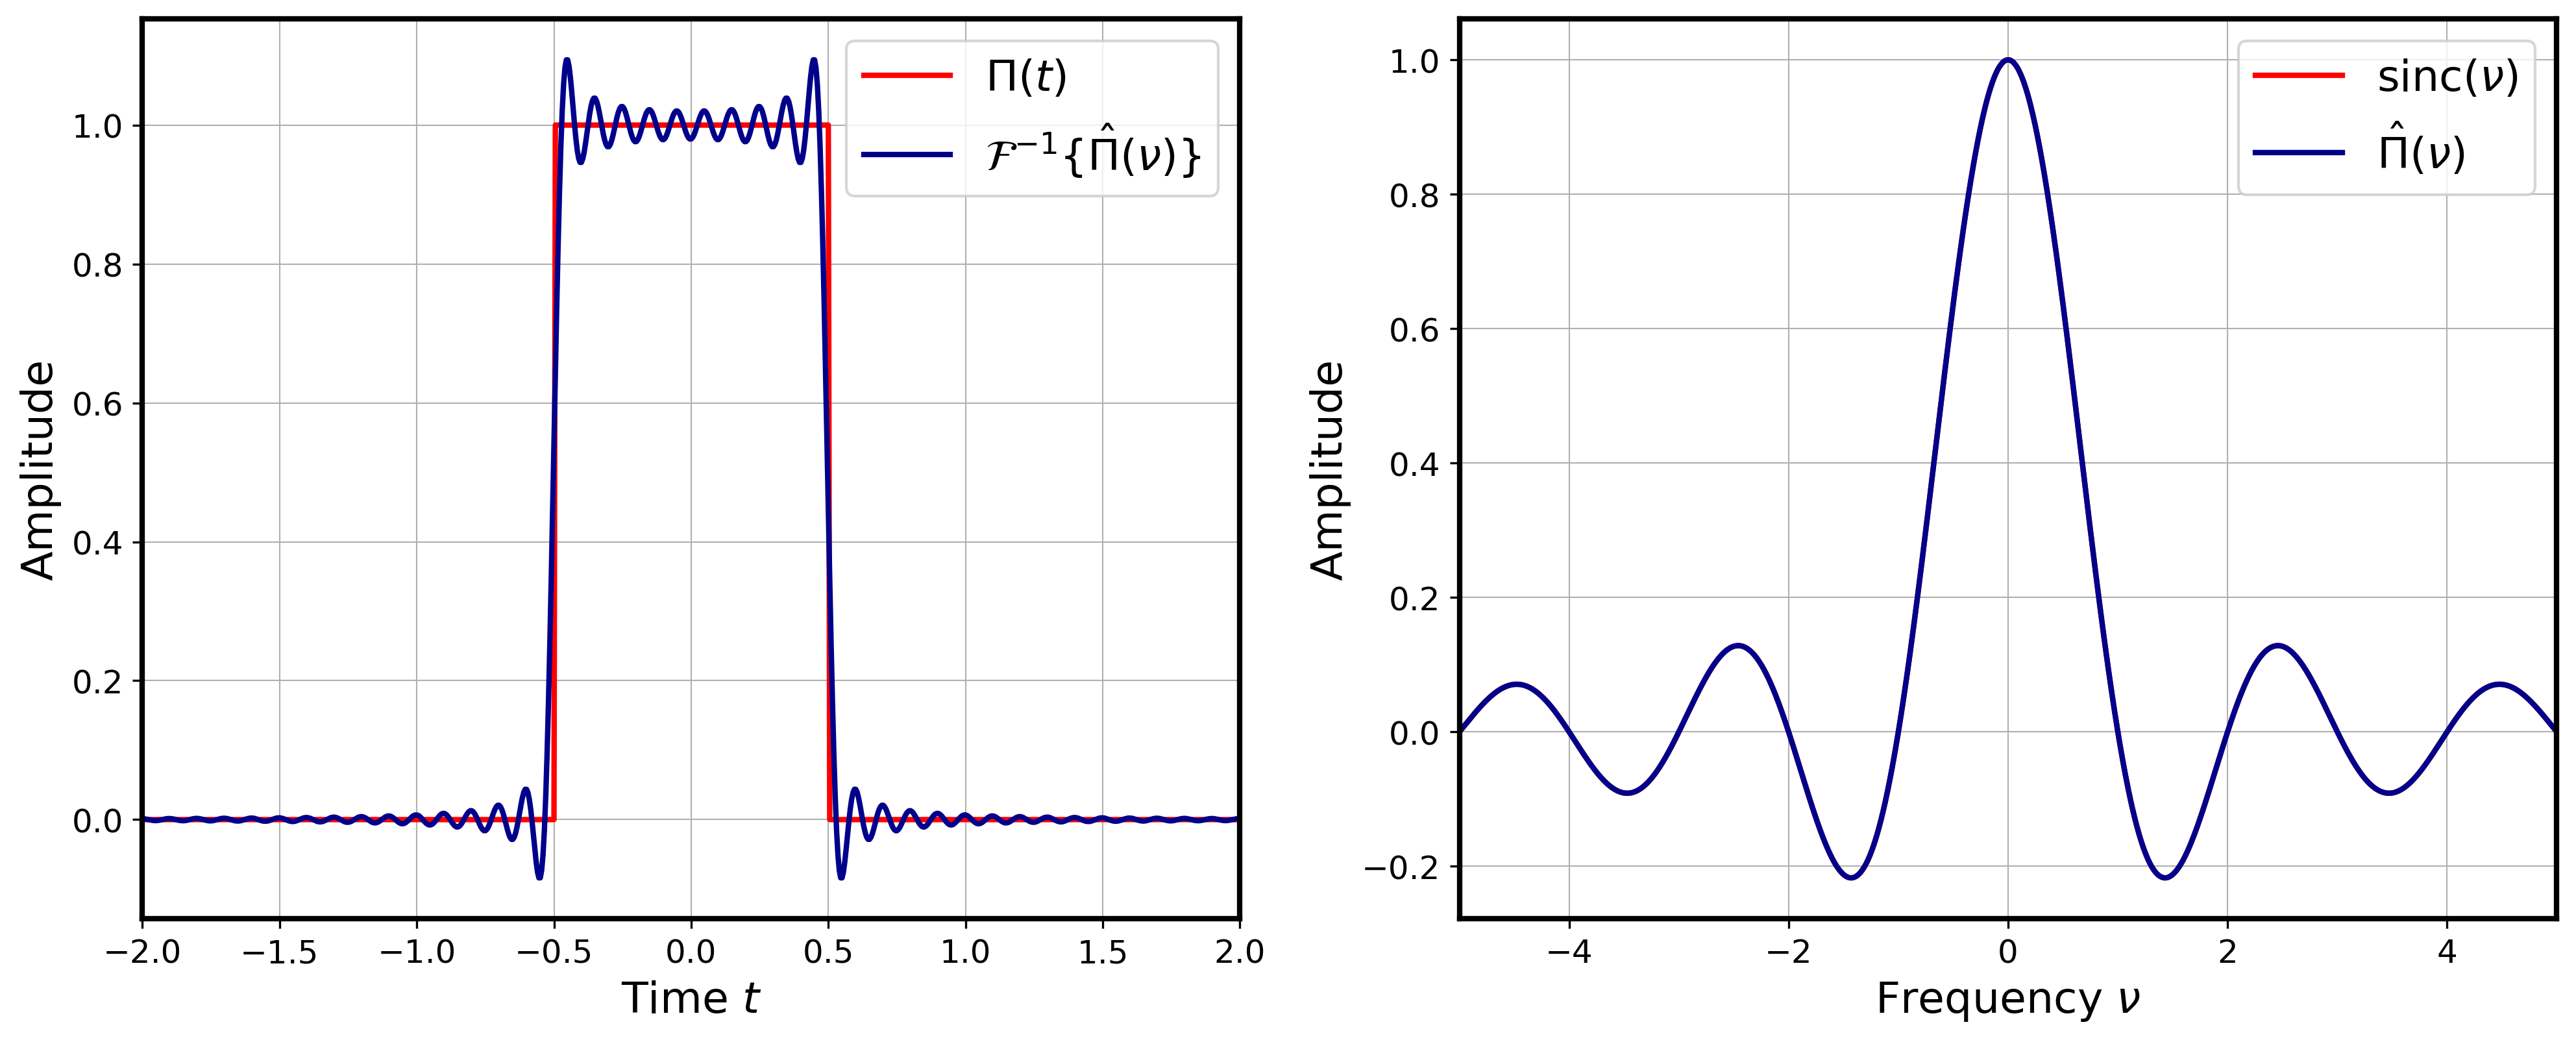
\includegraphics[width=1\textwidth]{../images/task1/combined_T_20_dt_0.005_V_20_dnu_0.005.png} 
	\caption{Графики функций и фурье-образов}
\end{figure}

Время выполнения цикла (время построения двух графиков со всеми расчетами) заняло 6.5 секунд. 

\subsubsection{Влияние параметра \(T\)}

Исследую влияние параметра \(T\). Возьму значения \(T \in [40, 10, 1]\) и посмотрю на изменения. Остальные значения: $\Delta t = 0.005$, $V = 20$, $\Delta \nu = 0.005$ - остануться прежними.


\begin{figure}[H]
	\centering
	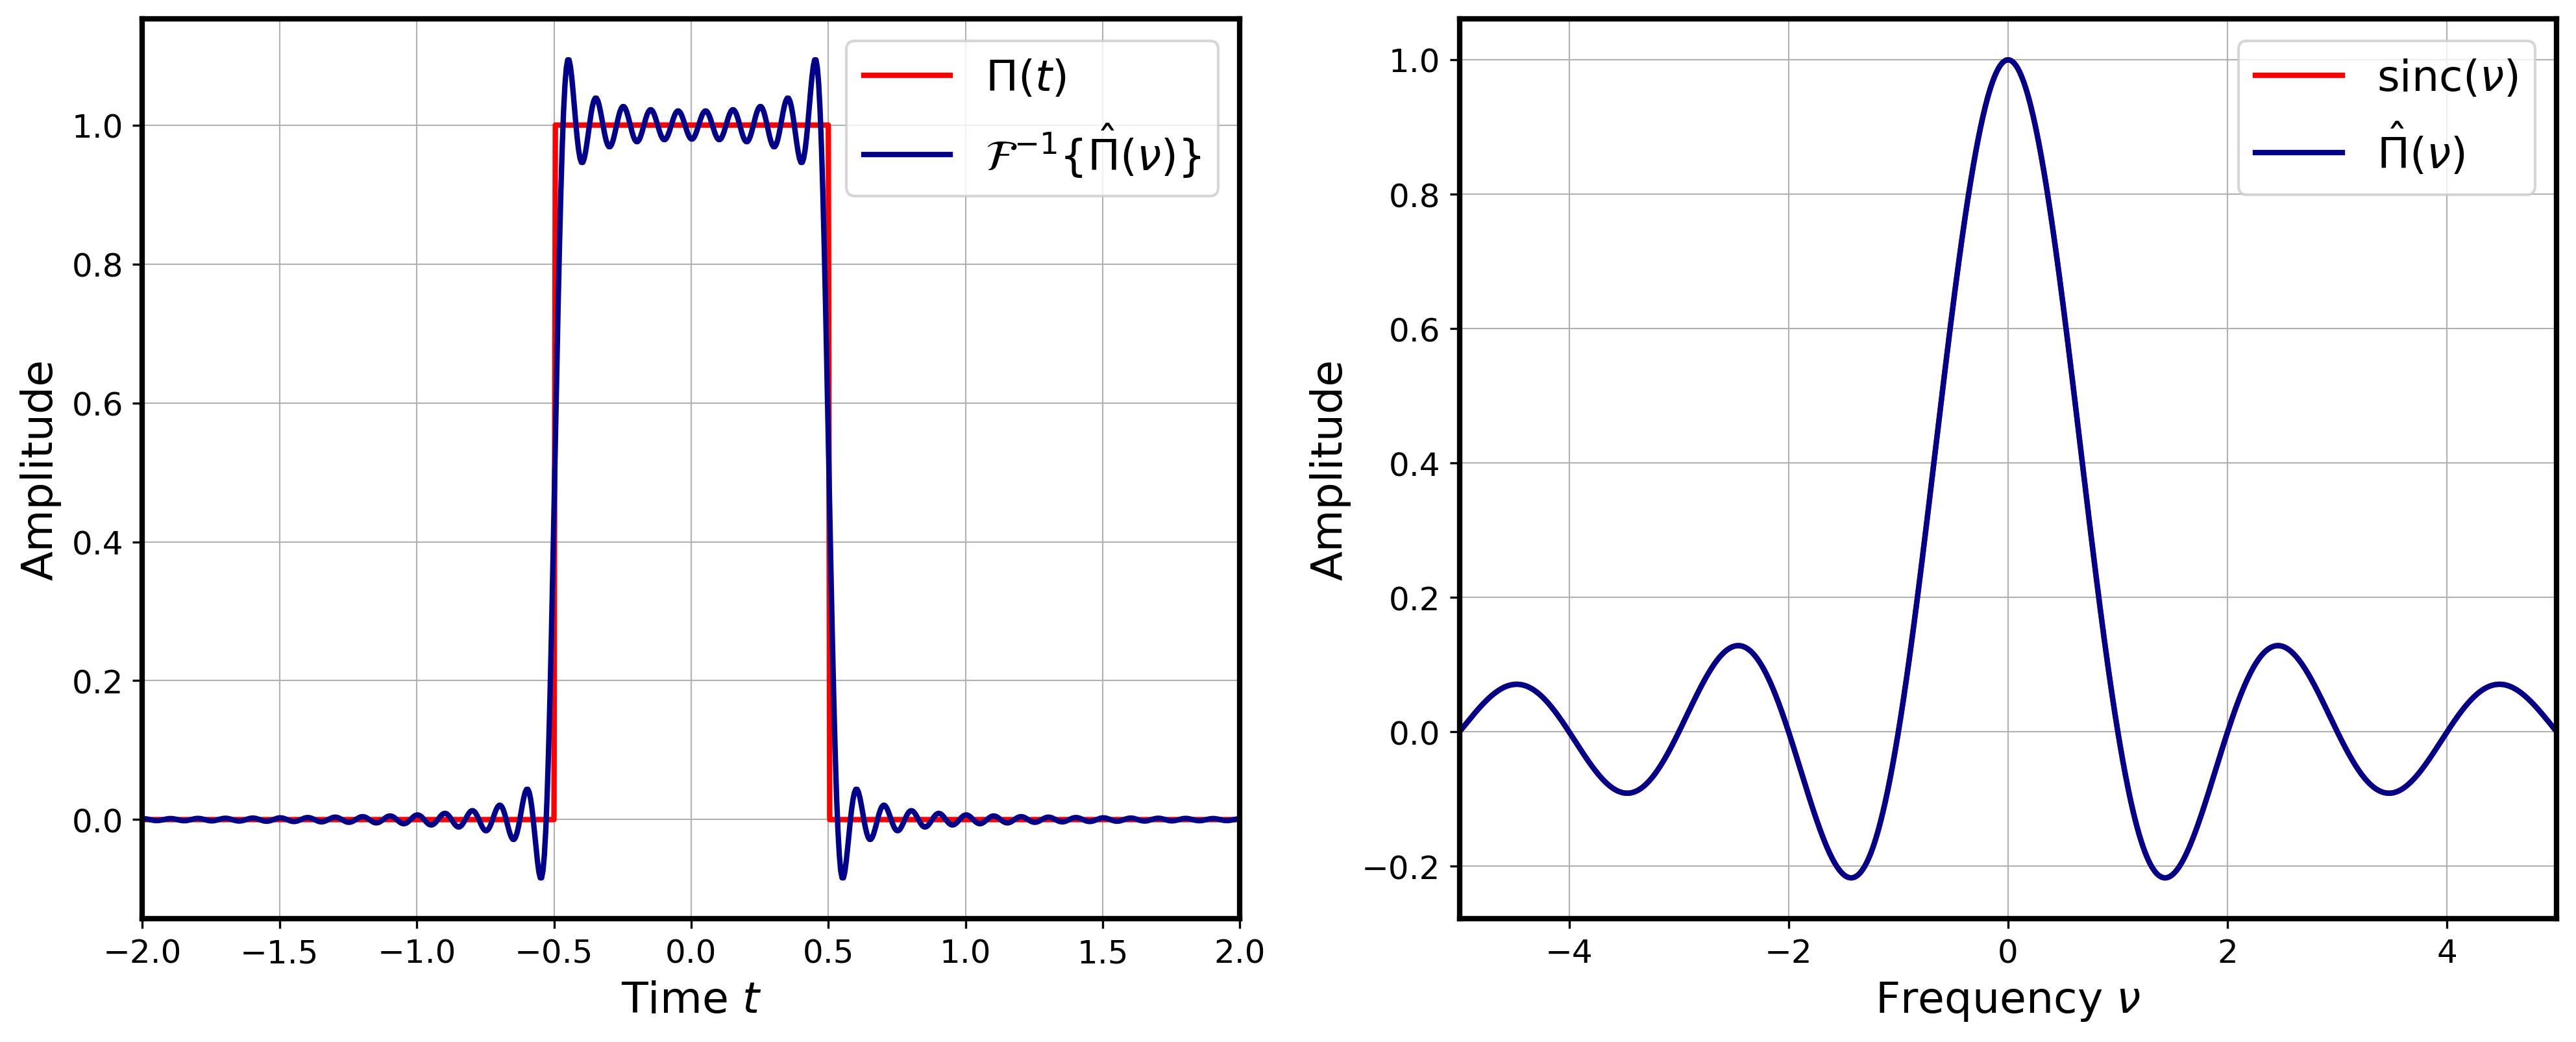
\includegraphics[width=1\textwidth]{../images/task1/combined_T_40_dt_0.005_V_20_dnu_0.005.png} 
	\caption{Графики функций и фурье-образов. \(T = 40\).}
\end{figure}


\begin{figure}[H]
	\centering
	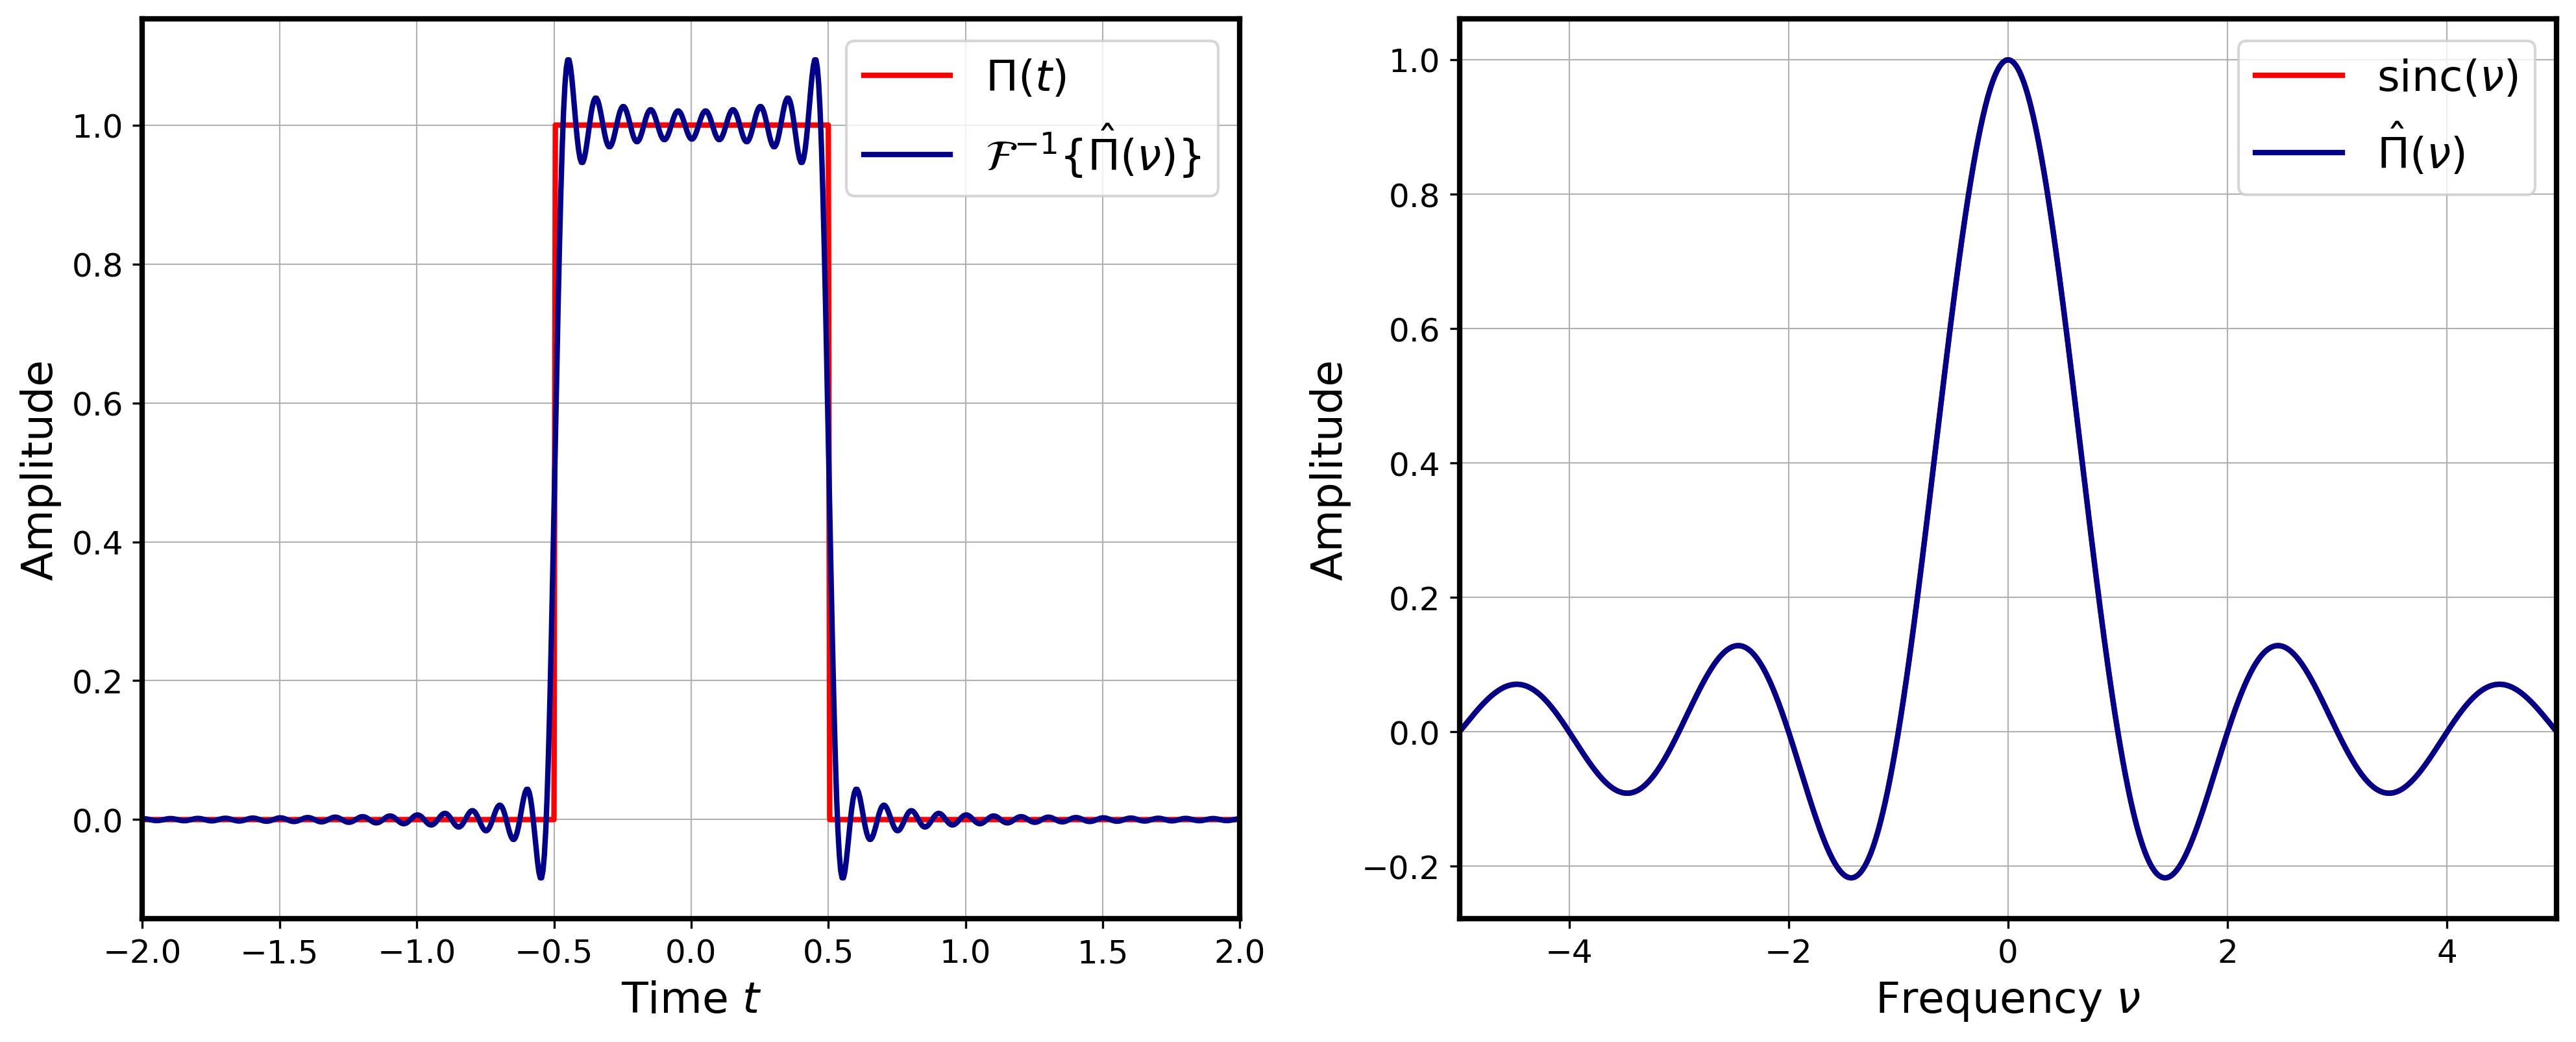
\includegraphics[width=1\textwidth]{../images/task1/combined_T_10_dt_0.005_V_20_dnu_0.005.png} 
	\caption{Графики функций и фурье-образов. \(T = 10\).}
\end{figure}
		
Время выполнения - 4.1 секунды.

	
\begin{figure}[H]
	\centering
	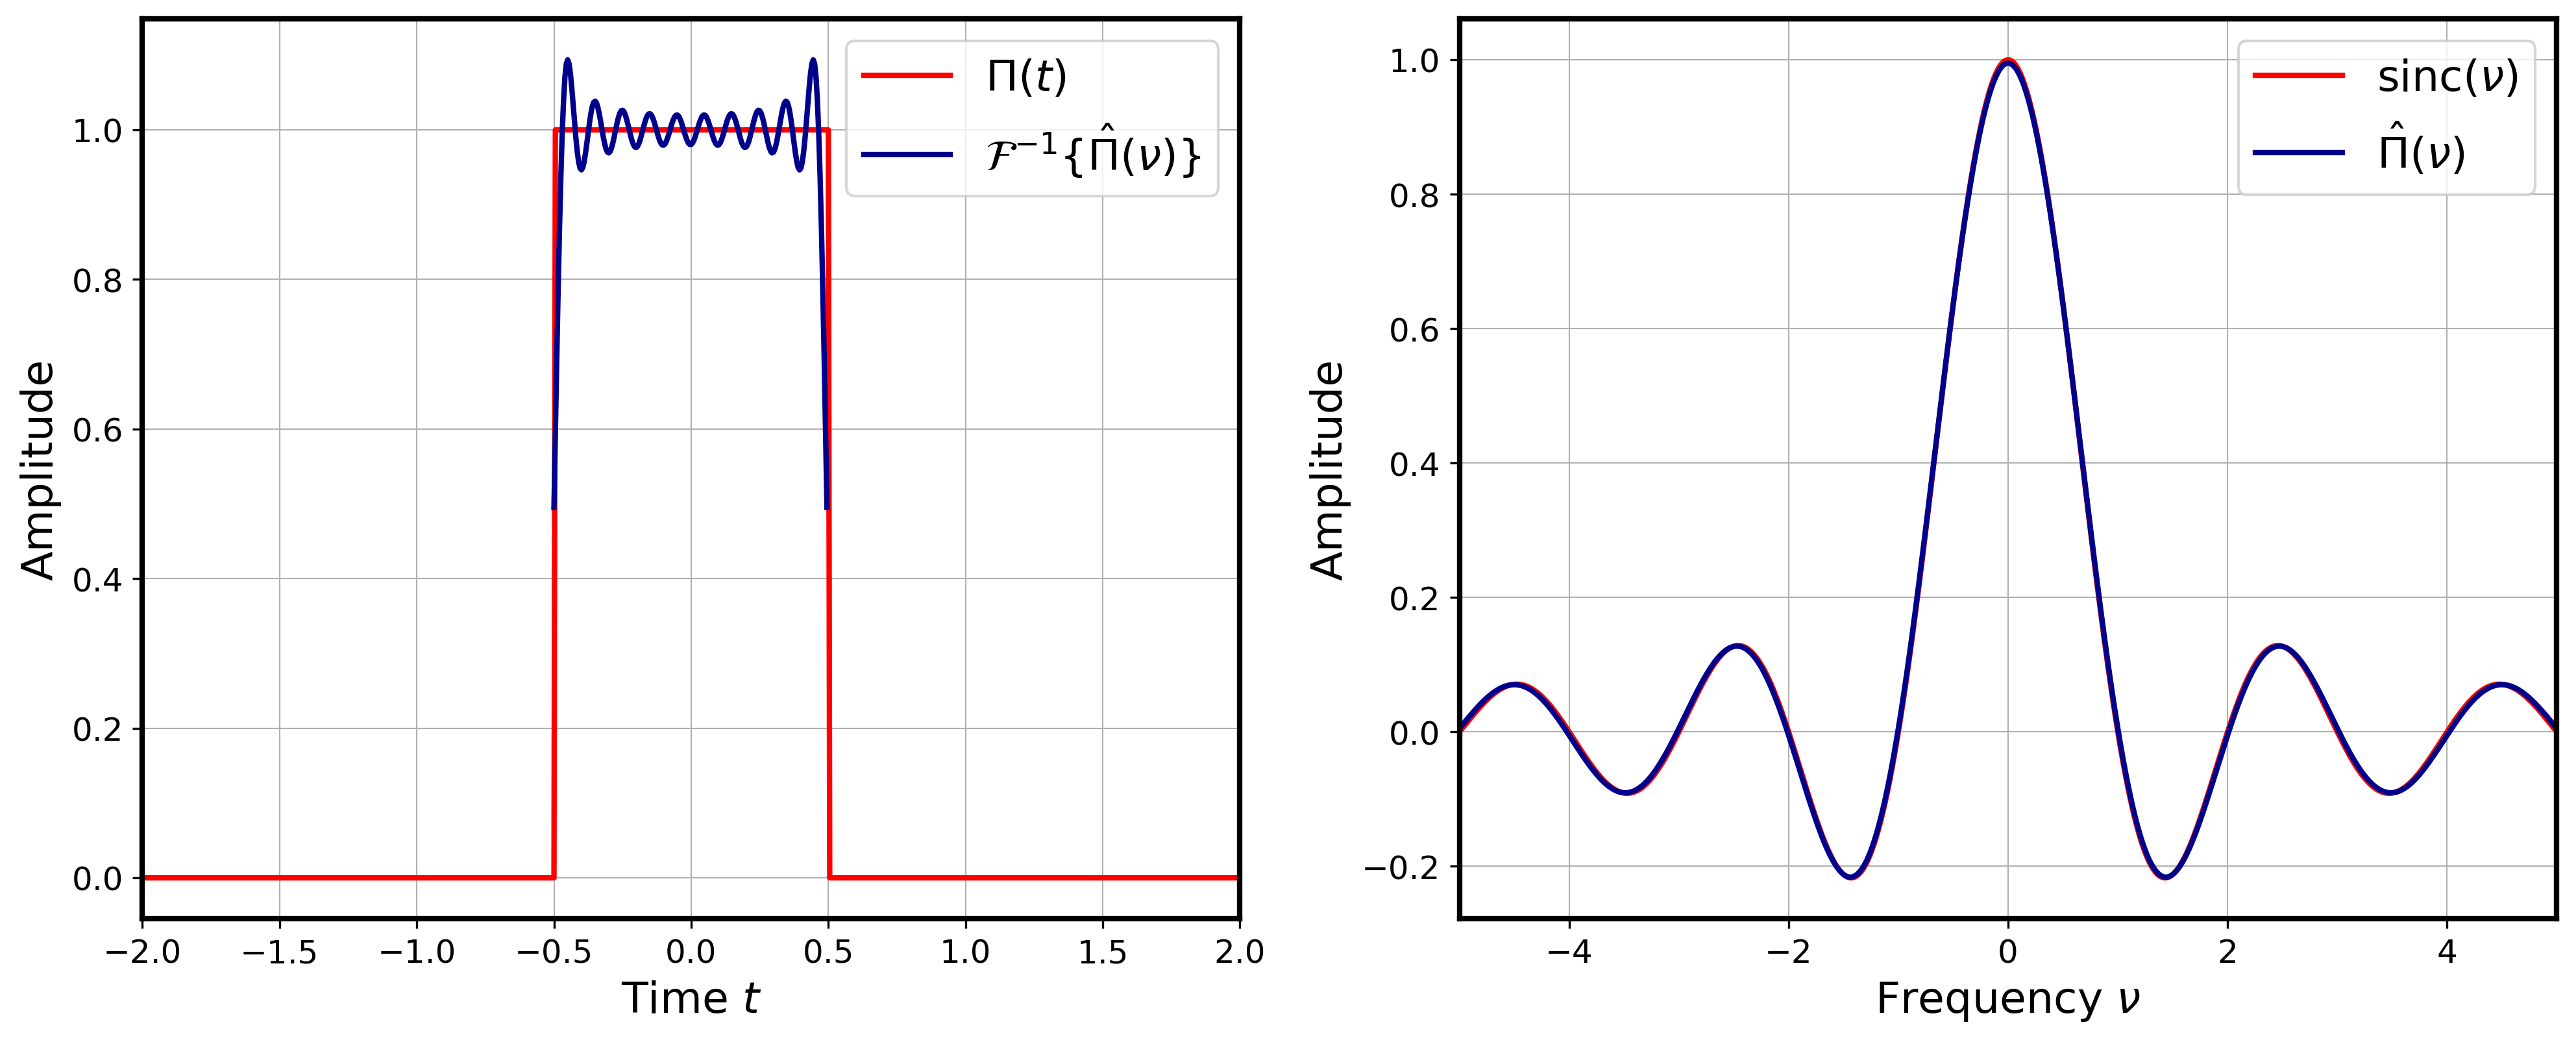
\includegraphics[width=1\textwidth]{../images/task1/combined_T_1_dt_0.005_V_20_dnu_0.005.png} 
	\caption{Графики функций и фурье-образов. \(T = 1\).}
\end{figure}

Время выполнения - 2.8 секунды.


\[\]


\textbf{Итог:} Параметр \(T\) определяет временной интервал реконструкции сигнала. С увеличением \(T\) возрастает время вычислений (с 2.8 с при \(T = 1\) до 10.2 с при \(T = 40\), однако это не приводит к ослаблению эффекта Гиббса. Эффект сохраняется на краях разрыва функции независимо от величины параметра.	


\subsubsection{Влияние параметра \(\Delta t\)}

Исследую влияние параметра \(\Delta t\). Возьму значения \(\Delta t \in [0.01, 0.1, 0.4]\) и посмотрю на изменения. Остальные значения: $T = 20$, $V = 20$, $\Delta \nu = 0.005$ - останутся прежними.

\begin{figure}[H]
	\centering
	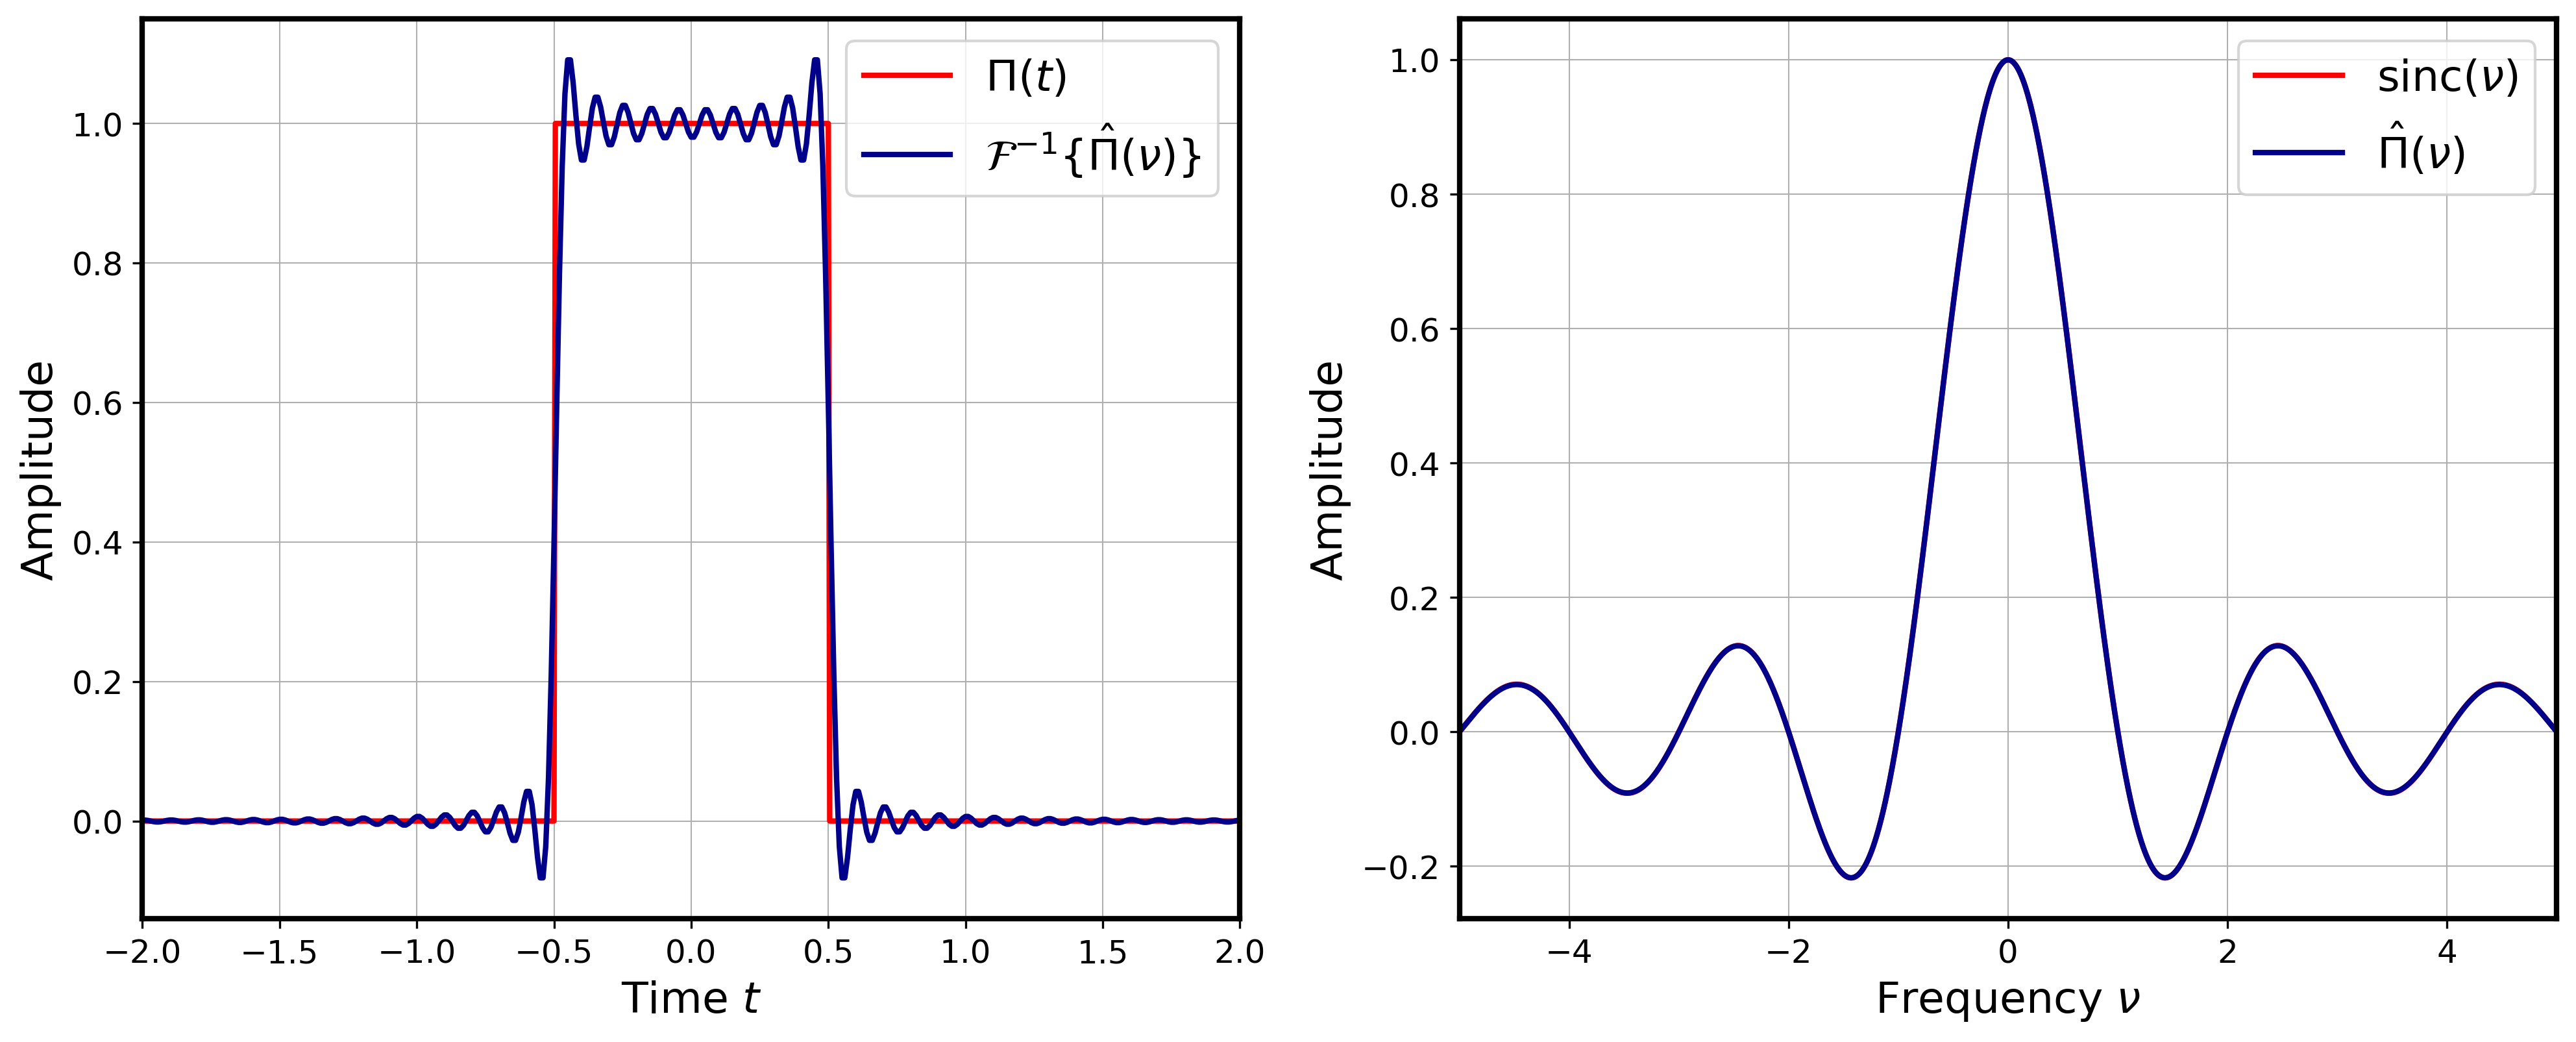
\includegraphics[width=1\textwidth]{../images/task1/combined_T_20_dt_0.01_V_20_dnu_0.005.png} 
	\caption{Графики функций и фурье-образов. \(\Delta t = 0.01\).}
\end{figure}

Время выполнения - 5.8 секунды.

\begin{figure}[H]
	\centering
	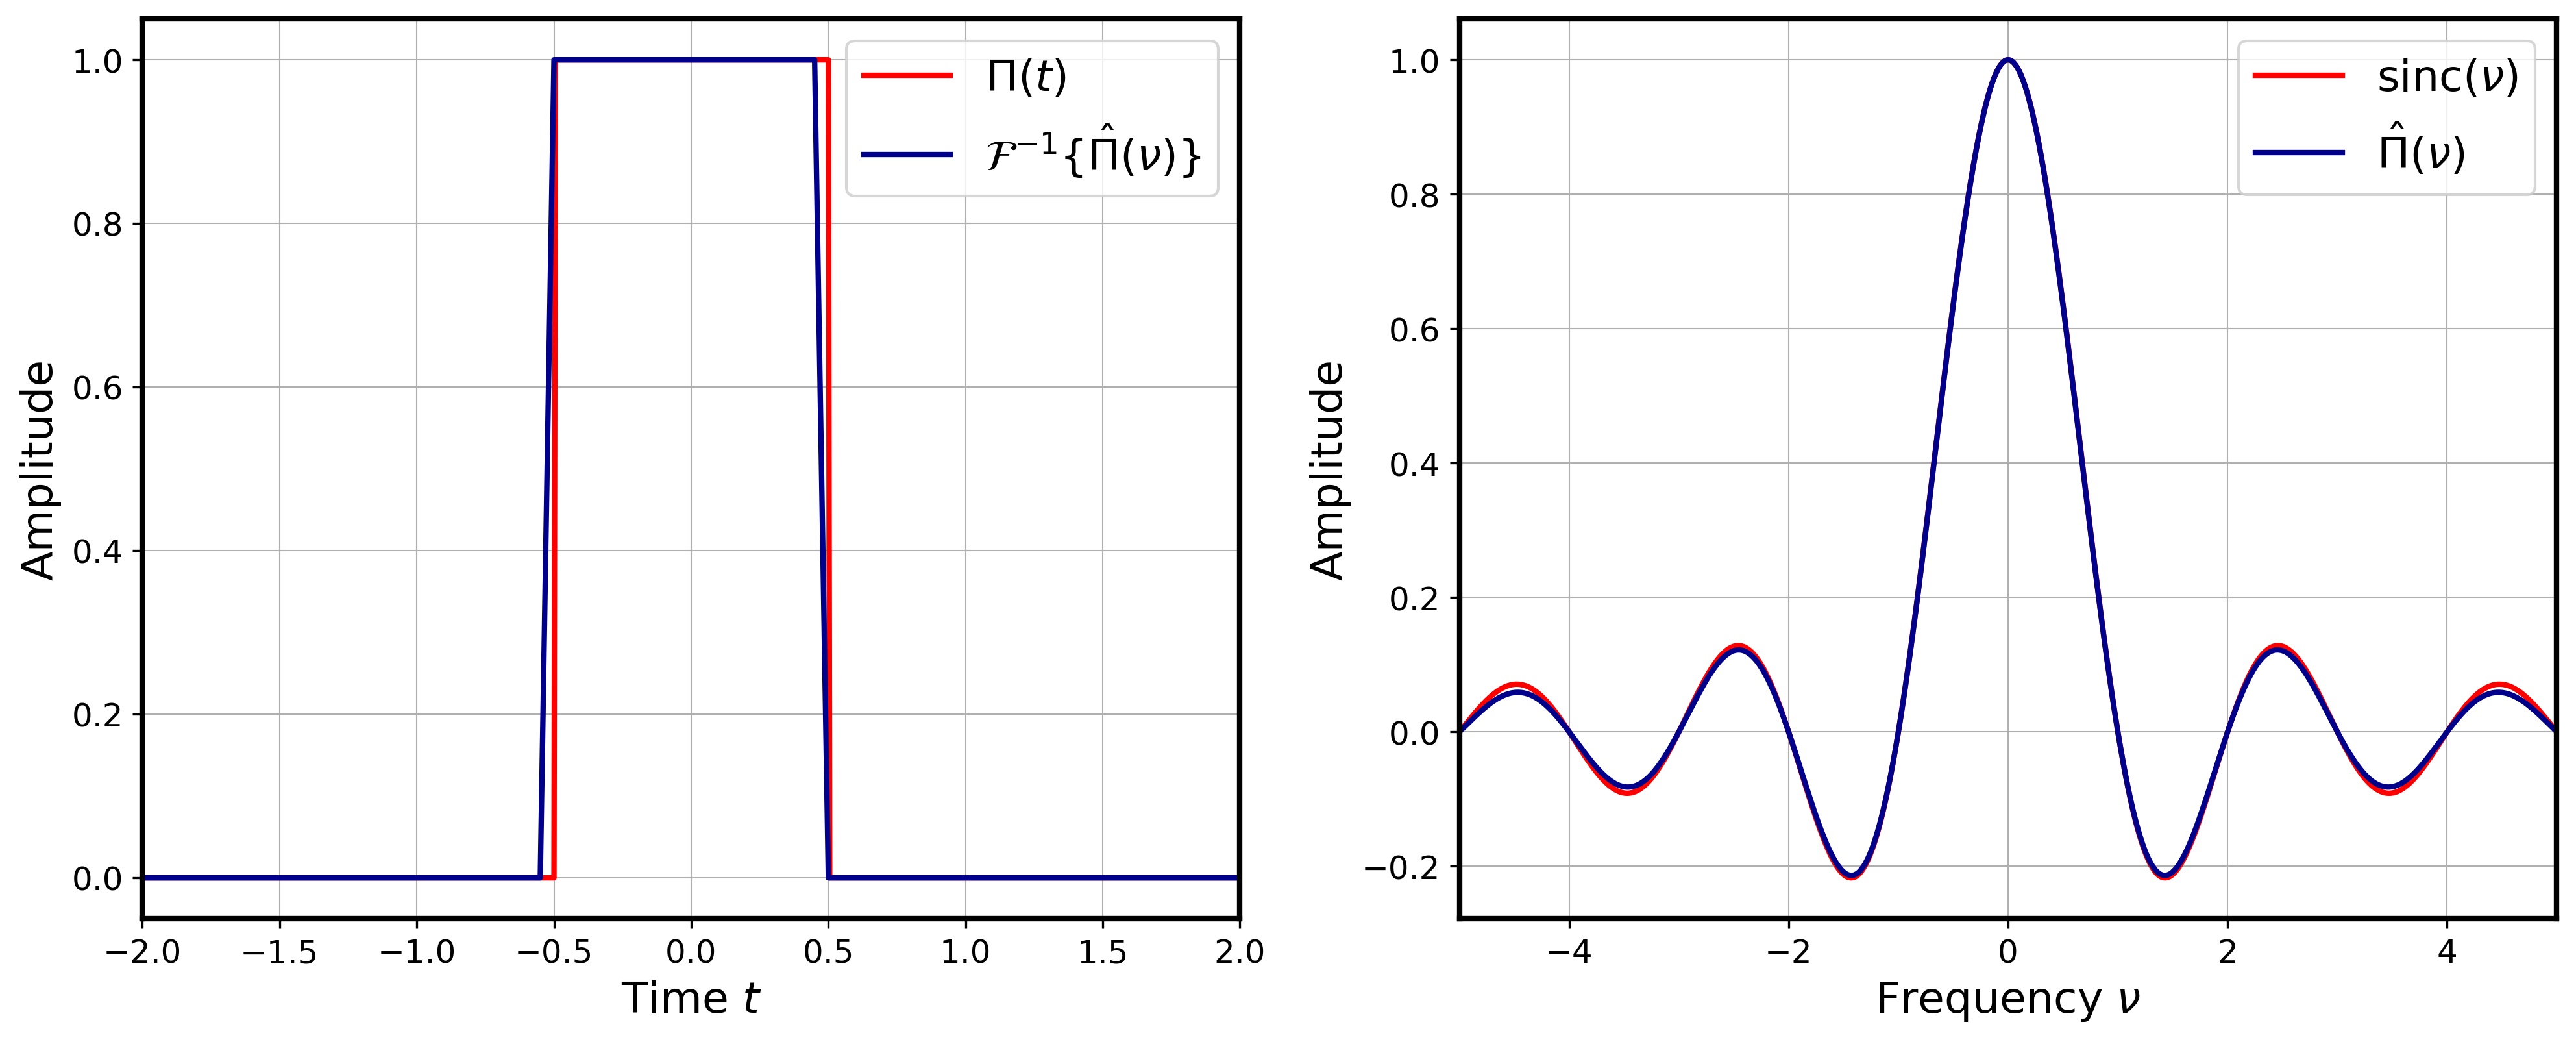
\includegraphics[width=1\textwidth]{../images/task1/combined_T_20_dt_0.05_V_20_dnu_0.005.png} 
	\caption{Графики функций и фурье-образов. \(\Delta t = 0.05\).}
\end{figure}

Время выполнения - 2.8 секунды.

\begin{figure}[H]
	\centering
	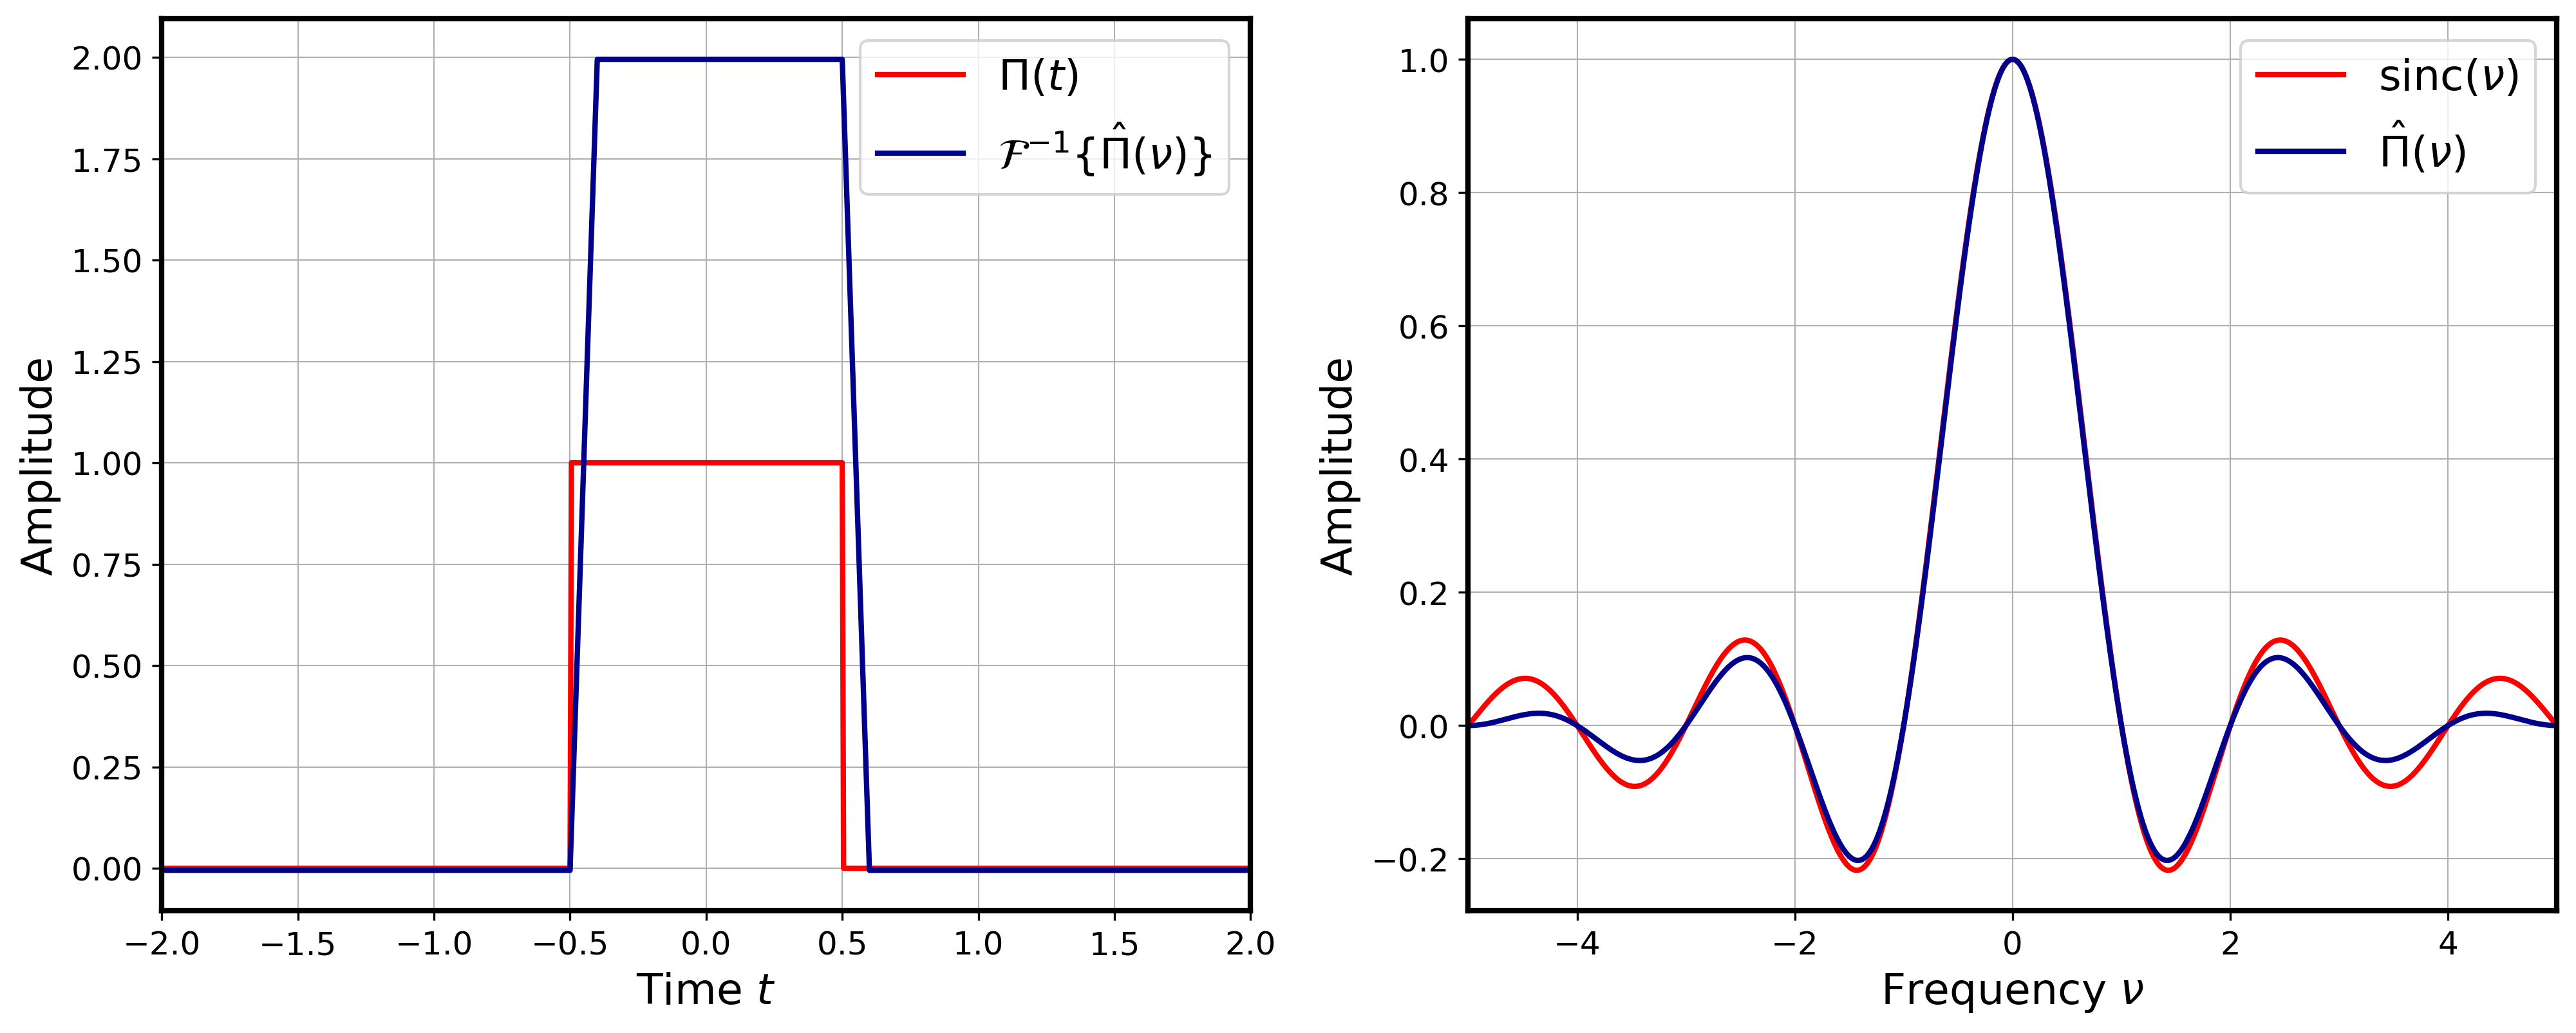
\includegraphics[width=1\textwidth]{../images/task1/combined_T_20_dt_0.1_V_20_dnu_0.005.png} 
	\caption{Графики функций и фурье-образов. \(\Delta t = 0.1\).}
\end{figure}

Время выполнения - 2.3 секунды.

\[\]

\textbf{Итог: } Экспериментально удалось выяснить, что при \(\Delta t >= 0.05\) у восстановленного сигнала исчезает эффект Гиббса и сигнал становится прямоугольным. Это связано с тем, что грубая дискретизация отсекает высокие частоты.  Однако если слишком сильно увеличить параметр у прямоугольного восстановленного сигнала значительно увеличится амплитуда.

\subsubsection{Влияние параметра \(V\)}

Исследую влияние параметра \(V\). Возьму значения \(V \in [10, 5, 1]\) и посмотрю на изменения. Остальные значения: $T = 20$, $\Delta t = 0.005$, $\Delta \nu = 0.005$ - останутся прежними.

\begin{figure}[H]
	\centering
	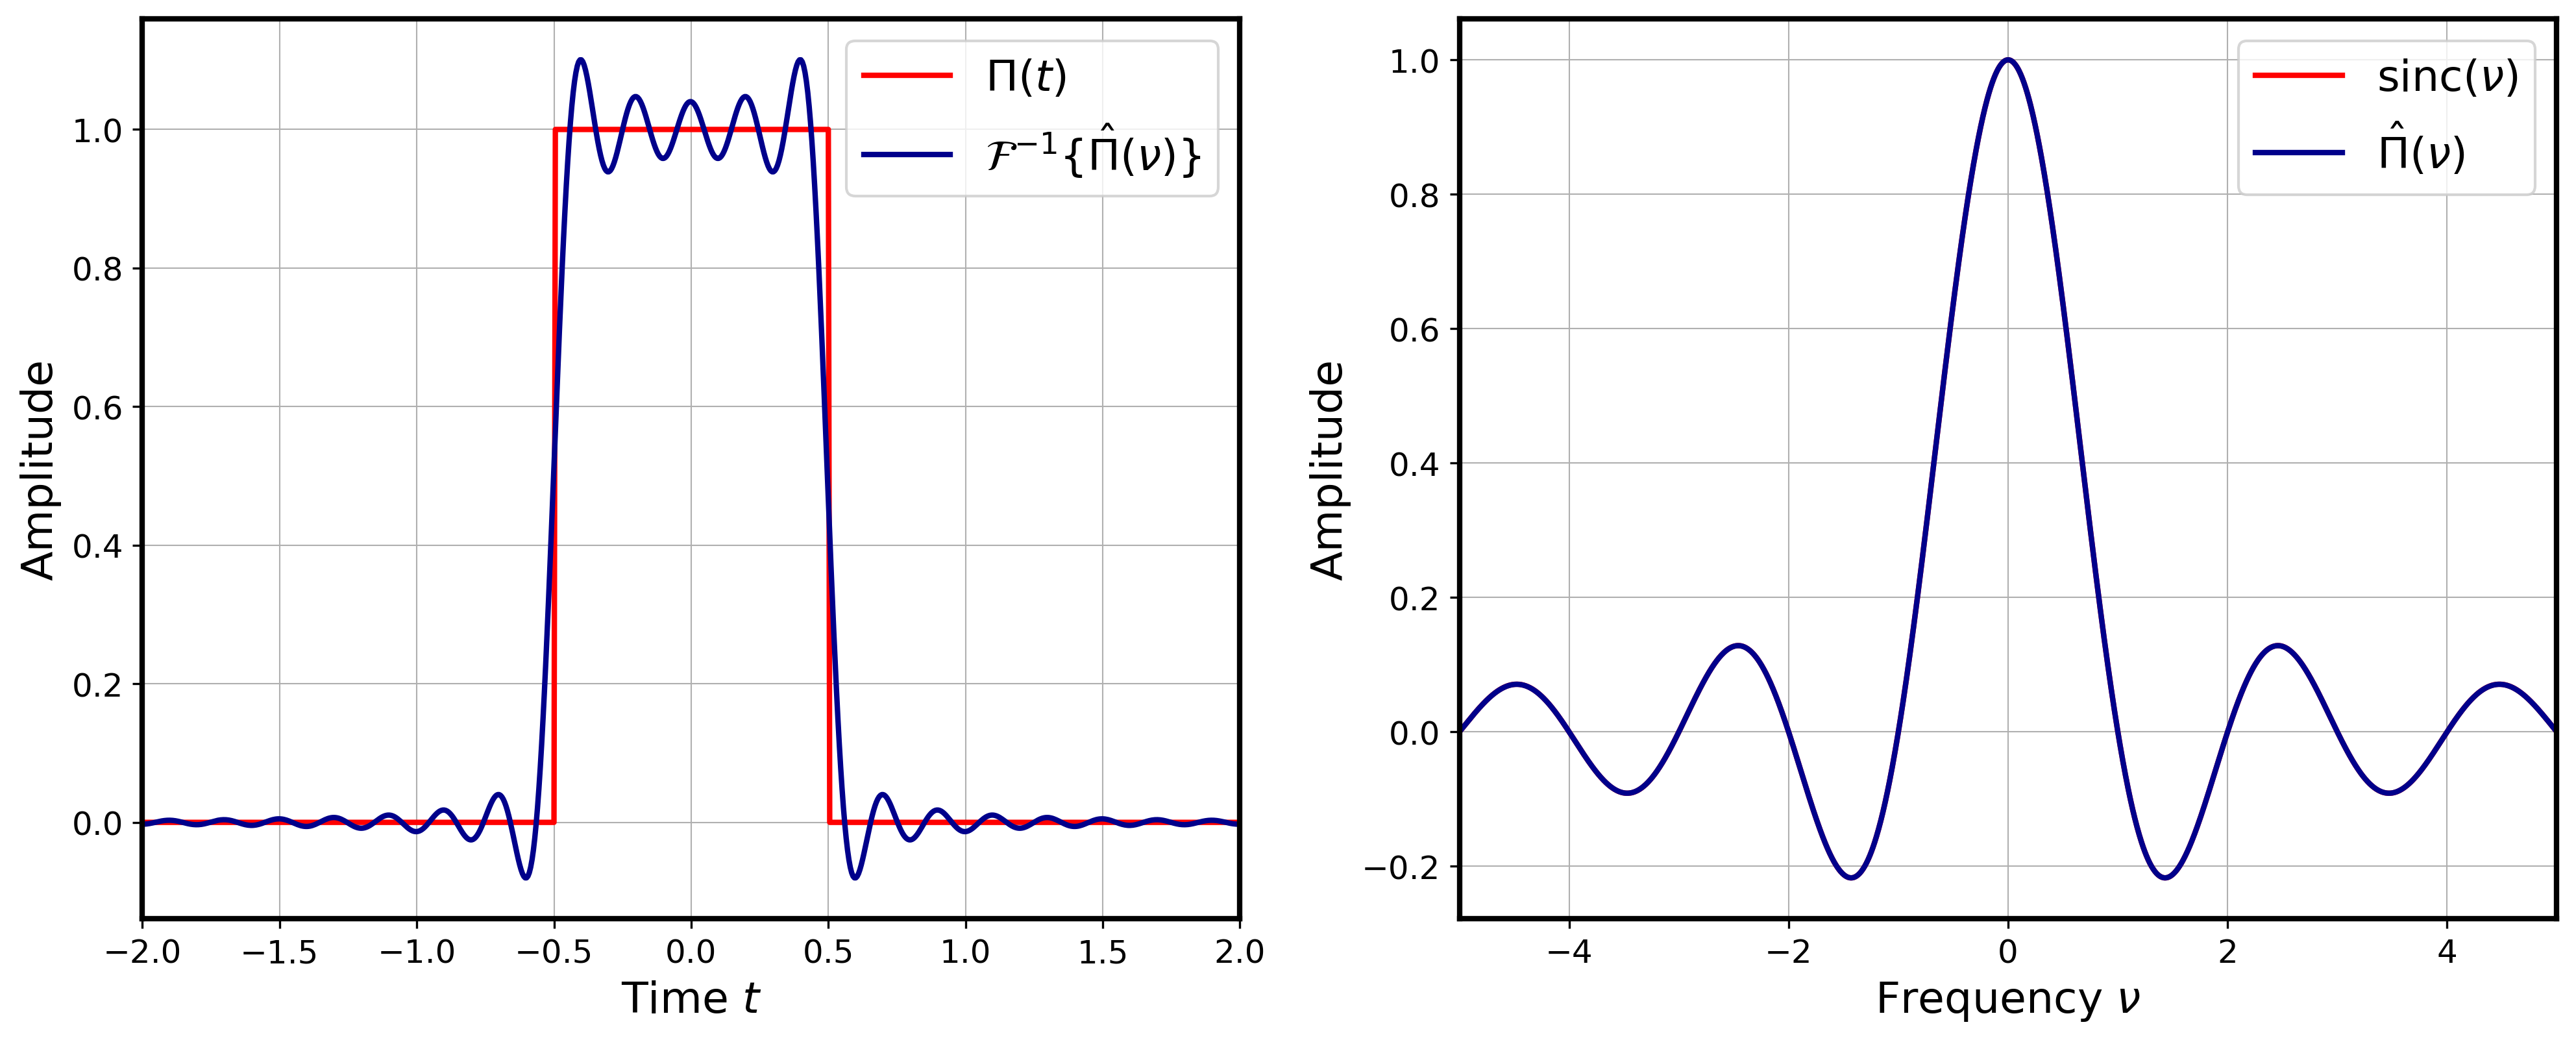
\includegraphics[width=1\textwidth]{../images/task1/combined_T_20_dt_0.005_V_10_dnu_0.005.png} 
	\caption{Графики функций и фурье-образов. \(V = 10\).}
\end{figure}

Время выполнения - 5.1 секунды.

\begin{figure}[H]
	\centering
	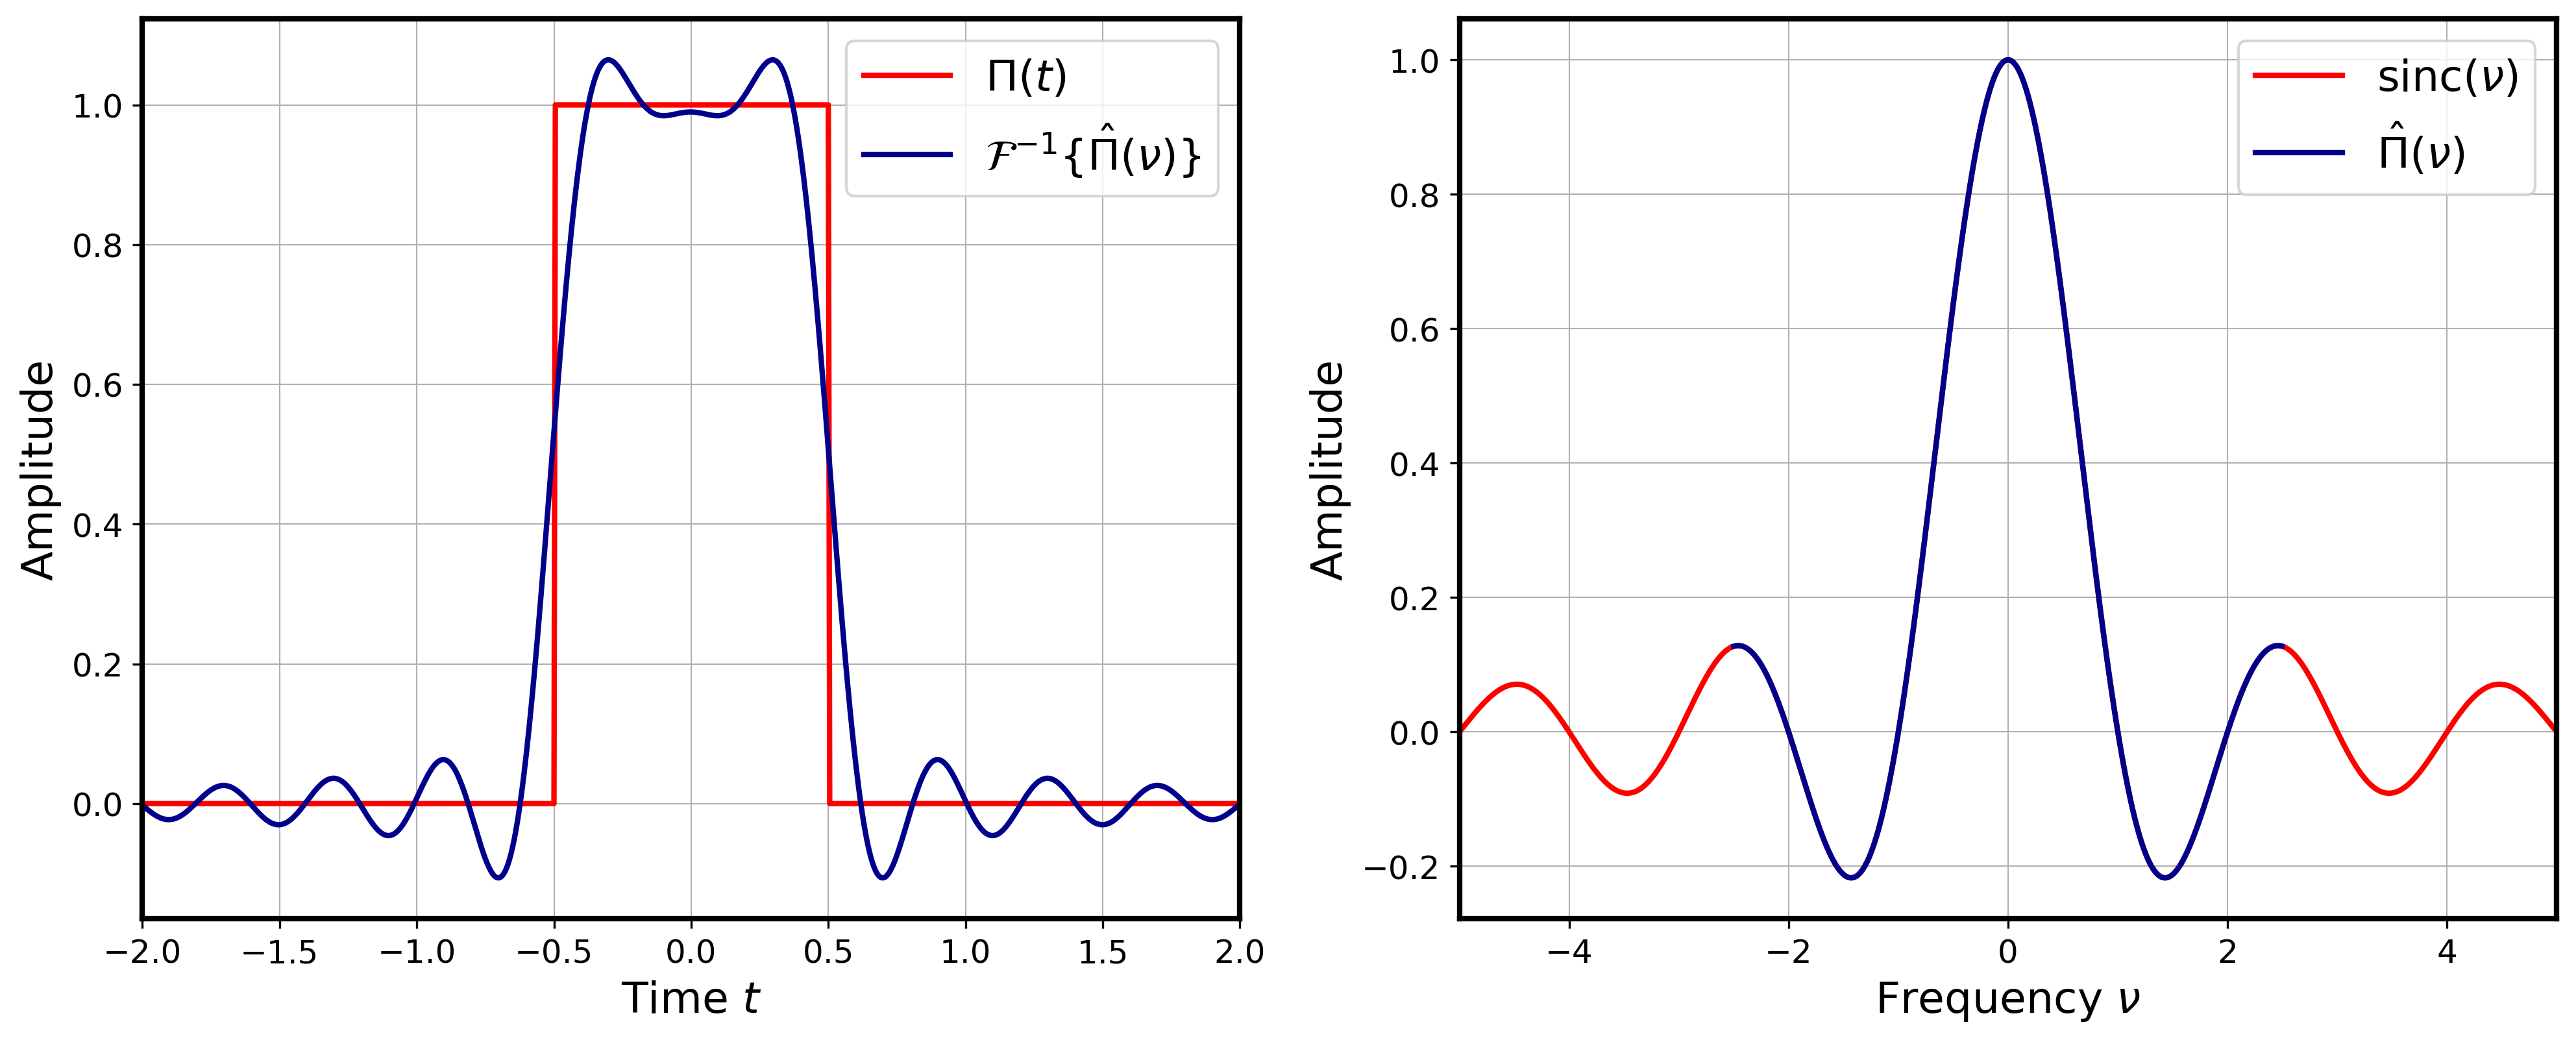
\includegraphics[width=1\textwidth]{../images/task1/combined_T_20_dt_0.005_V_5_dnu_0.005.png} 
	\caption{Графики функций и фурье-образов. \(V = 5\).}
\end{figure}

Время выполнения - 3.5 секунды.

\begin{figure}[H]
	\centering
	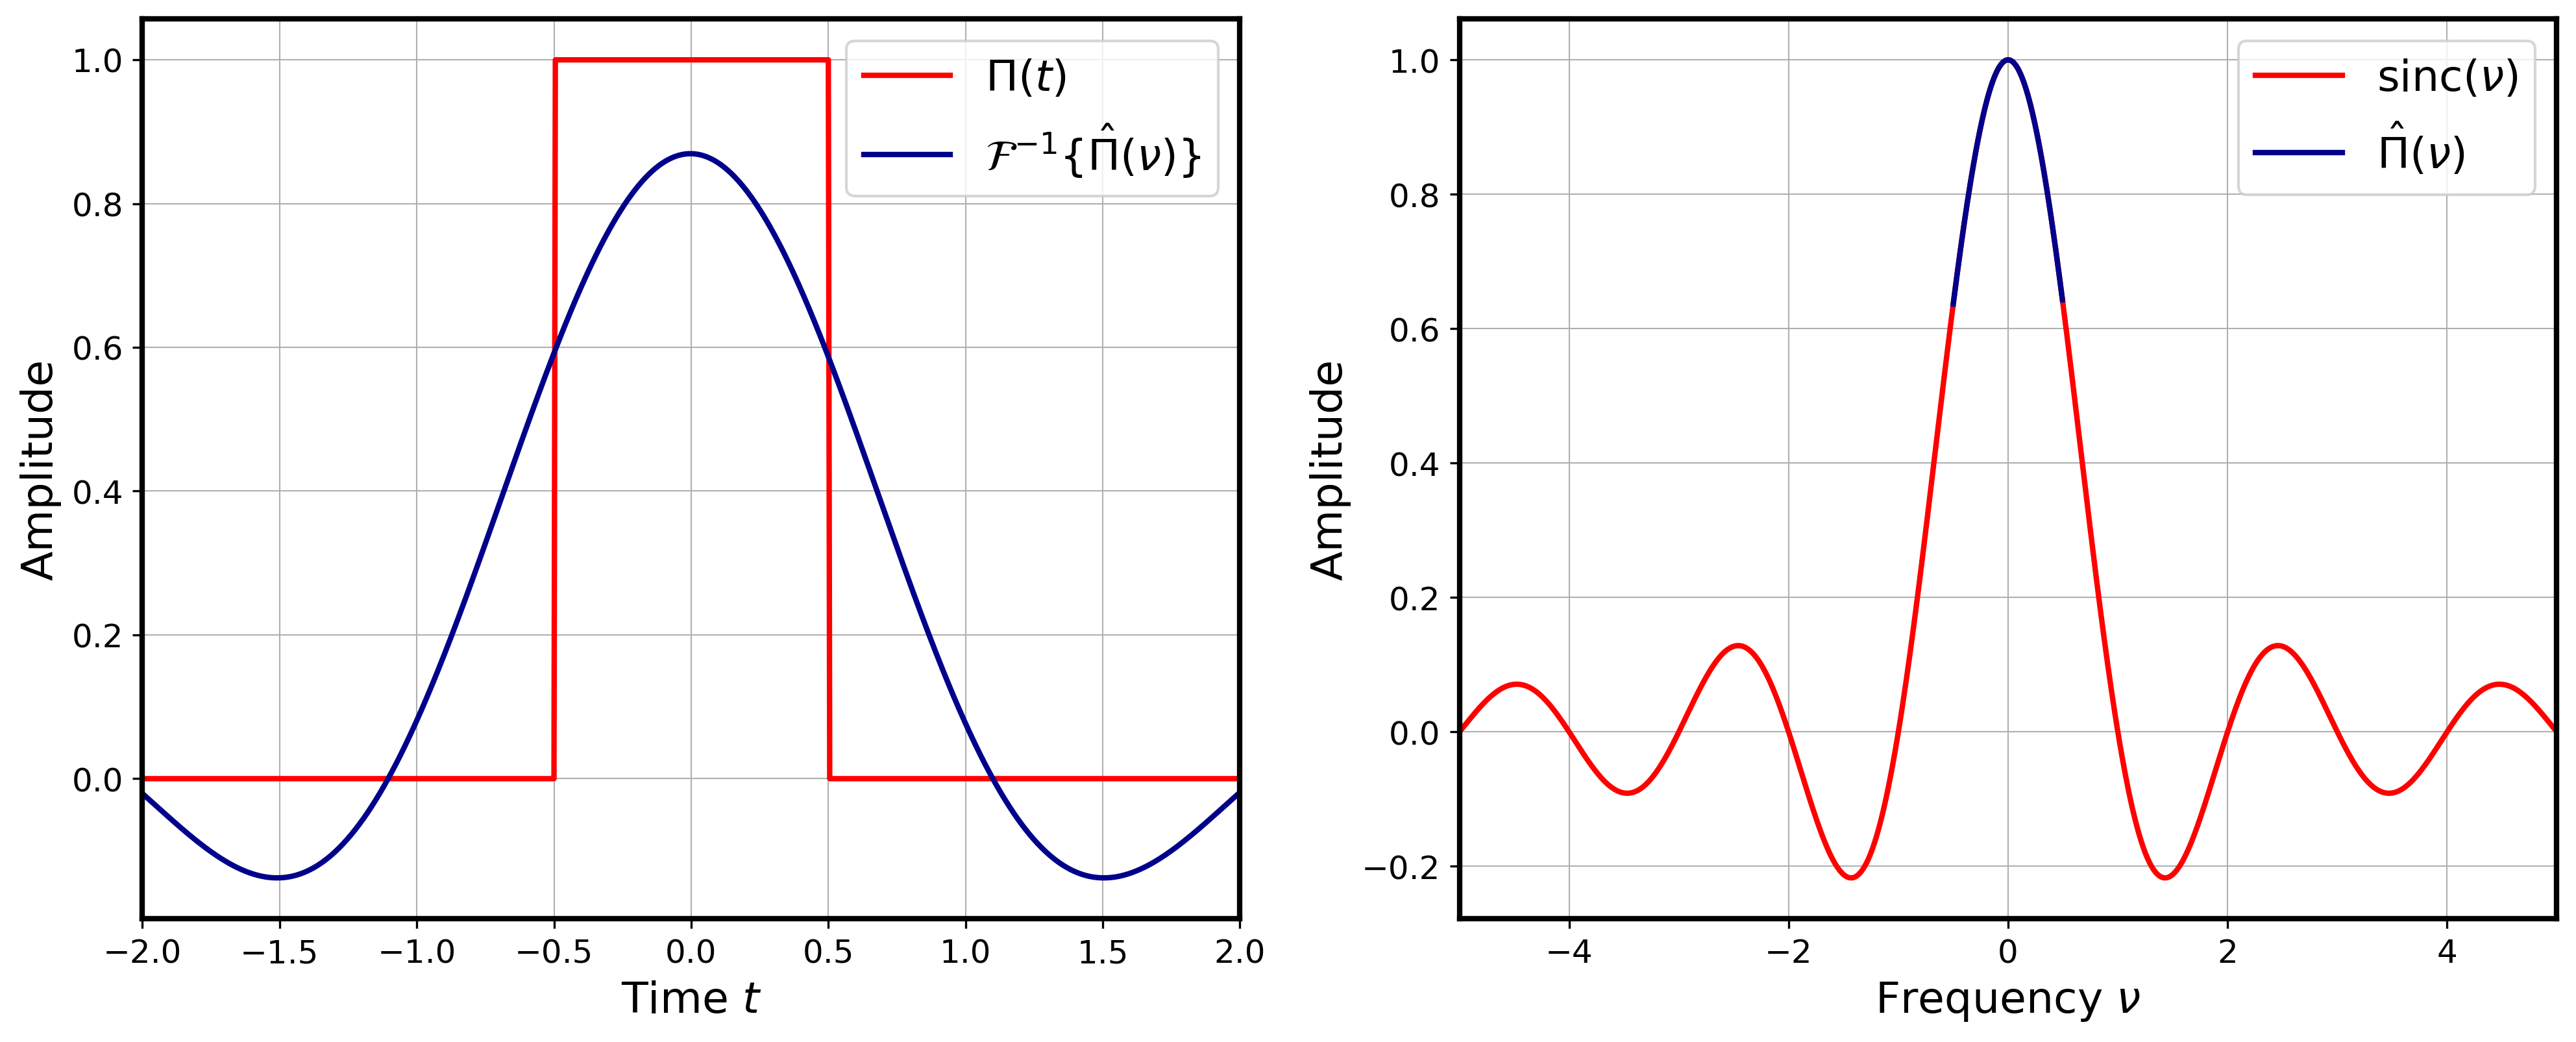
\includegraphics[width=1\textwidth]{../images/task1/combined_T_20_dt_0.005_V_1_dnu_0.005.png} 
	\caption{Графики функций и фурье-образов. \(V = 1\).}
\end{figure}

Время выполнения - 2.1 секунды.

\[\]

\textbf{Итог: } При уменьшении \(V\) происходит обрезание высокочастотных компонент спектра, что приводит к усилению эффекта Гиббса.

\subsubsection{Влияние параметра \(\Delta \nu\)}

Исследую влияние параметра \(\Delta \nu\). Возьму значения \(\Delta \nu \in [0.01, 0.01, 0.4]\) и посмотрю на изменения. Остальные значения: $T = 20$, $\Delta t = 0.005$, $V = 20$ - останутся прежними.

\begin{figure}[H]
	\centering
	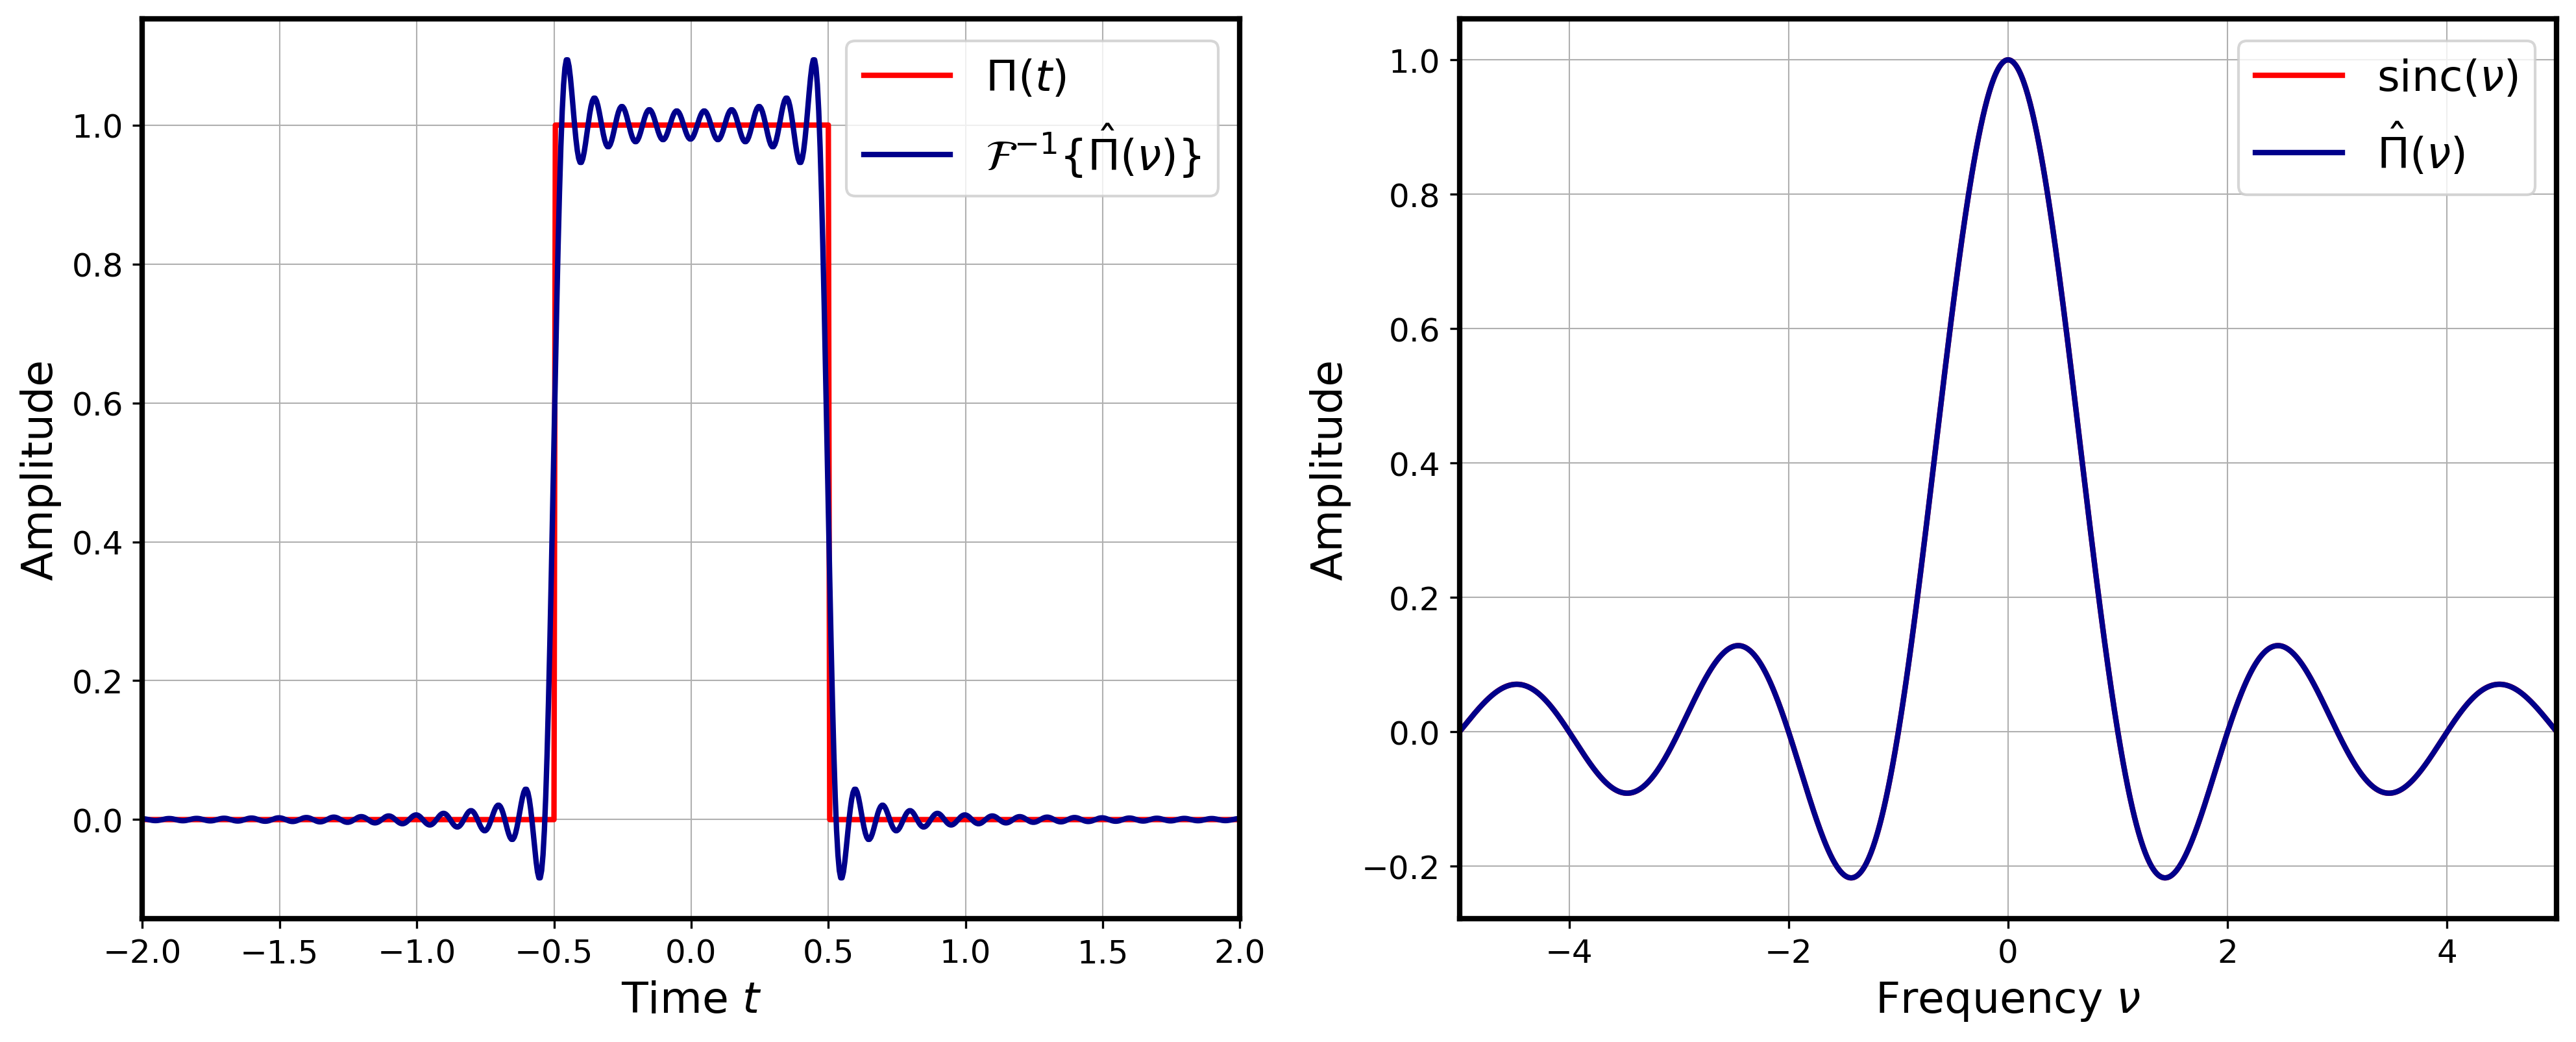
\includegraphics[width=1\textwidth]{../images/task1/combined_T_20_dt_0.005_V_20_dnu_0.01.png} 
	\caption{Графики функций и фурье-образов. \(\Delta \nu = 0.01\).}
\end{figure}

Время выполнения - 5.2 секунды.

\begin{figure}[H]
	\centering
	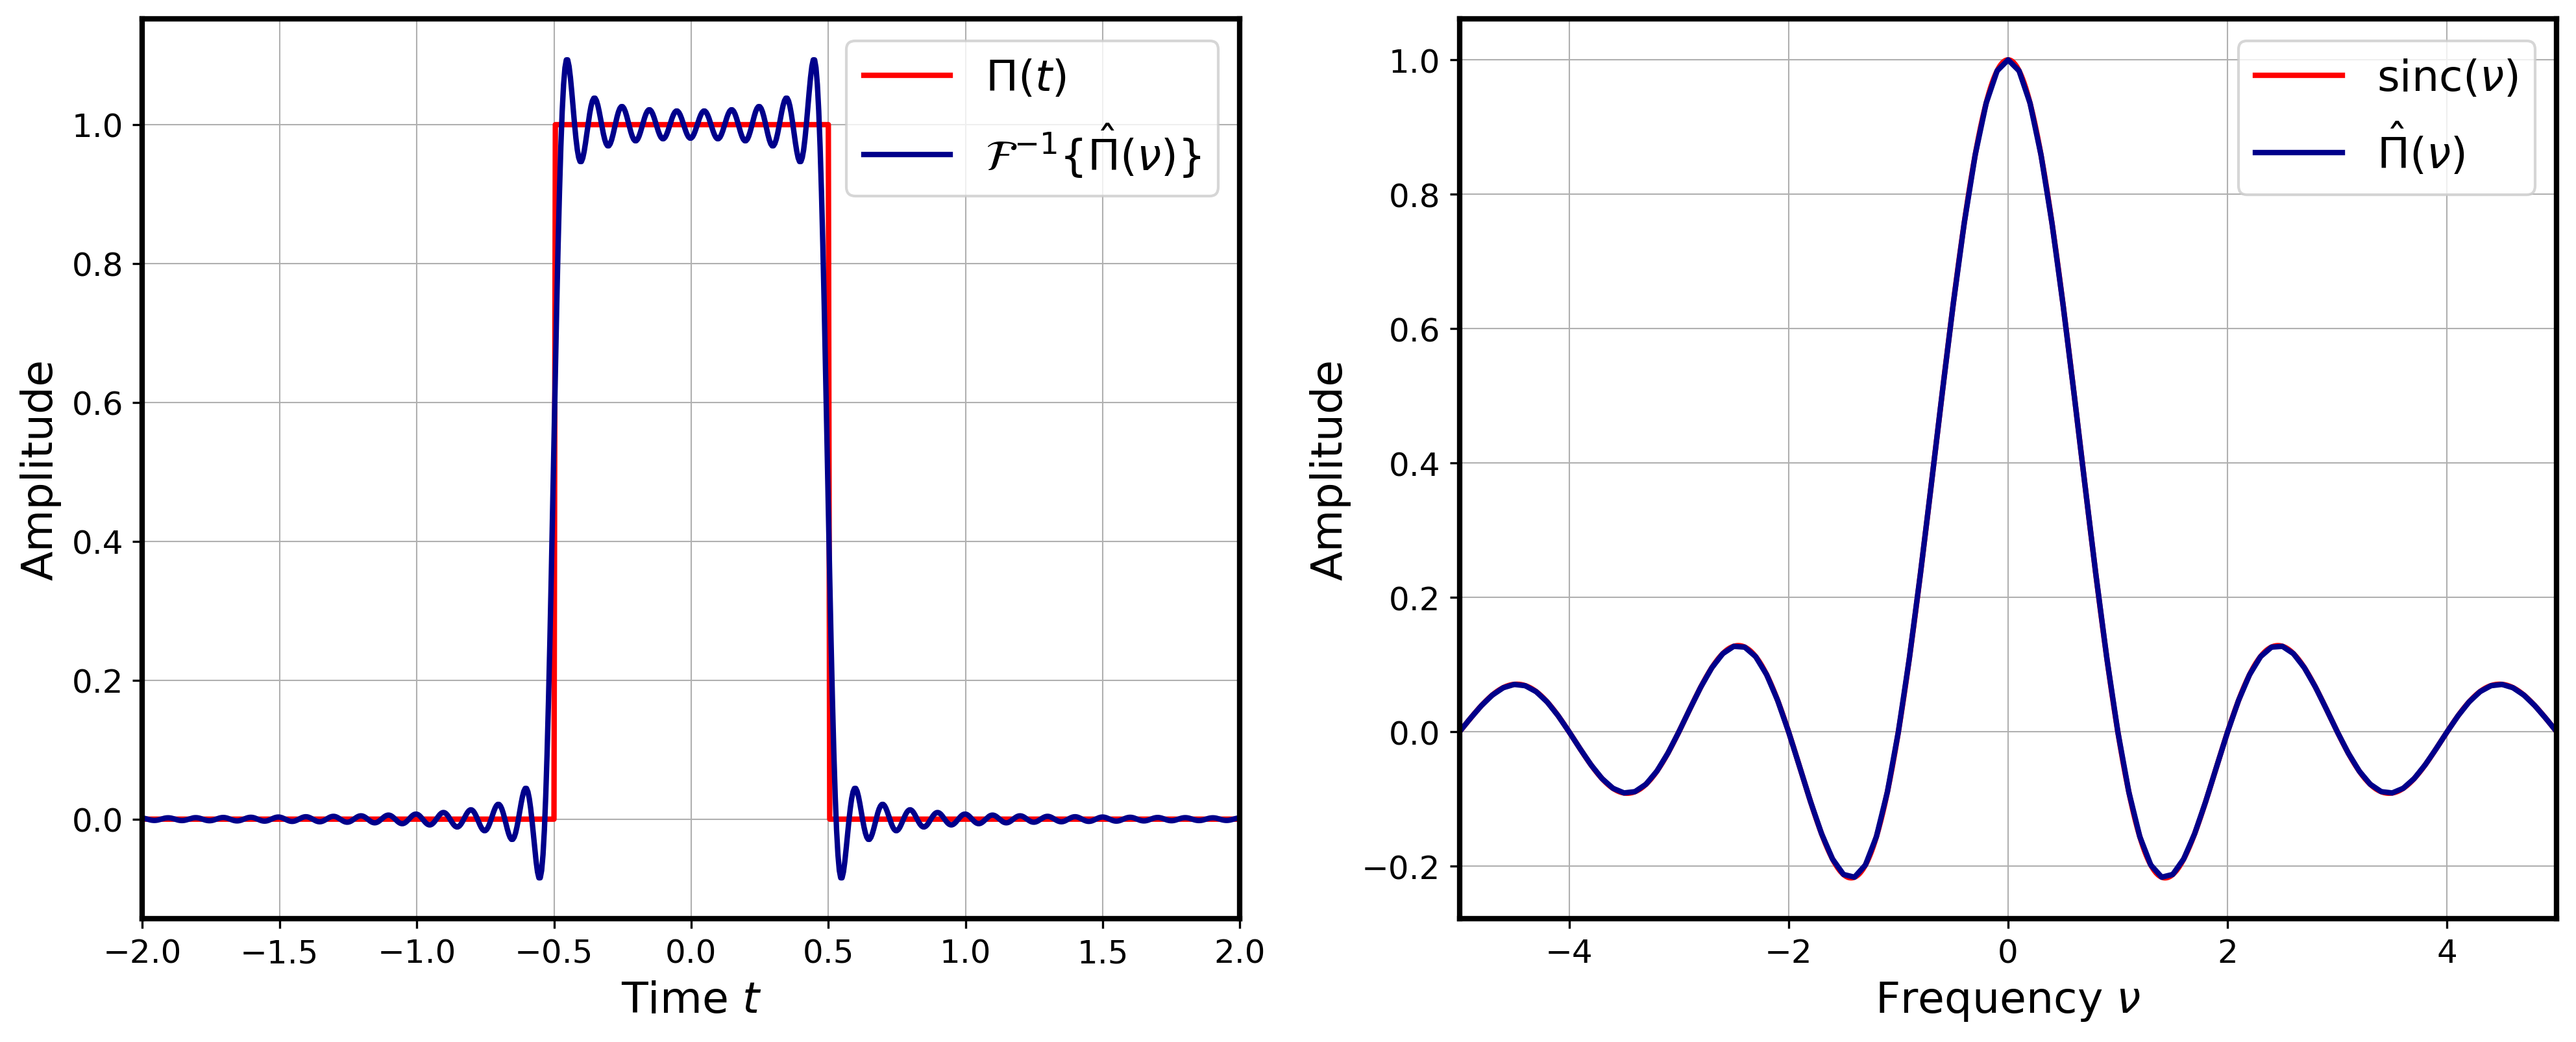
\includegraphics[width=1\textwidth]{../images/task1/combined_T_20_dt_0.005_V_20_dnu_0.1.png} 
	\caption{Графики функций и фурье-образов. \(\Delta \nu = 0.1\).}
\end{figure}


Время выполнения - 2.9 секунды.

\begin{figure}[H]
	\centering
	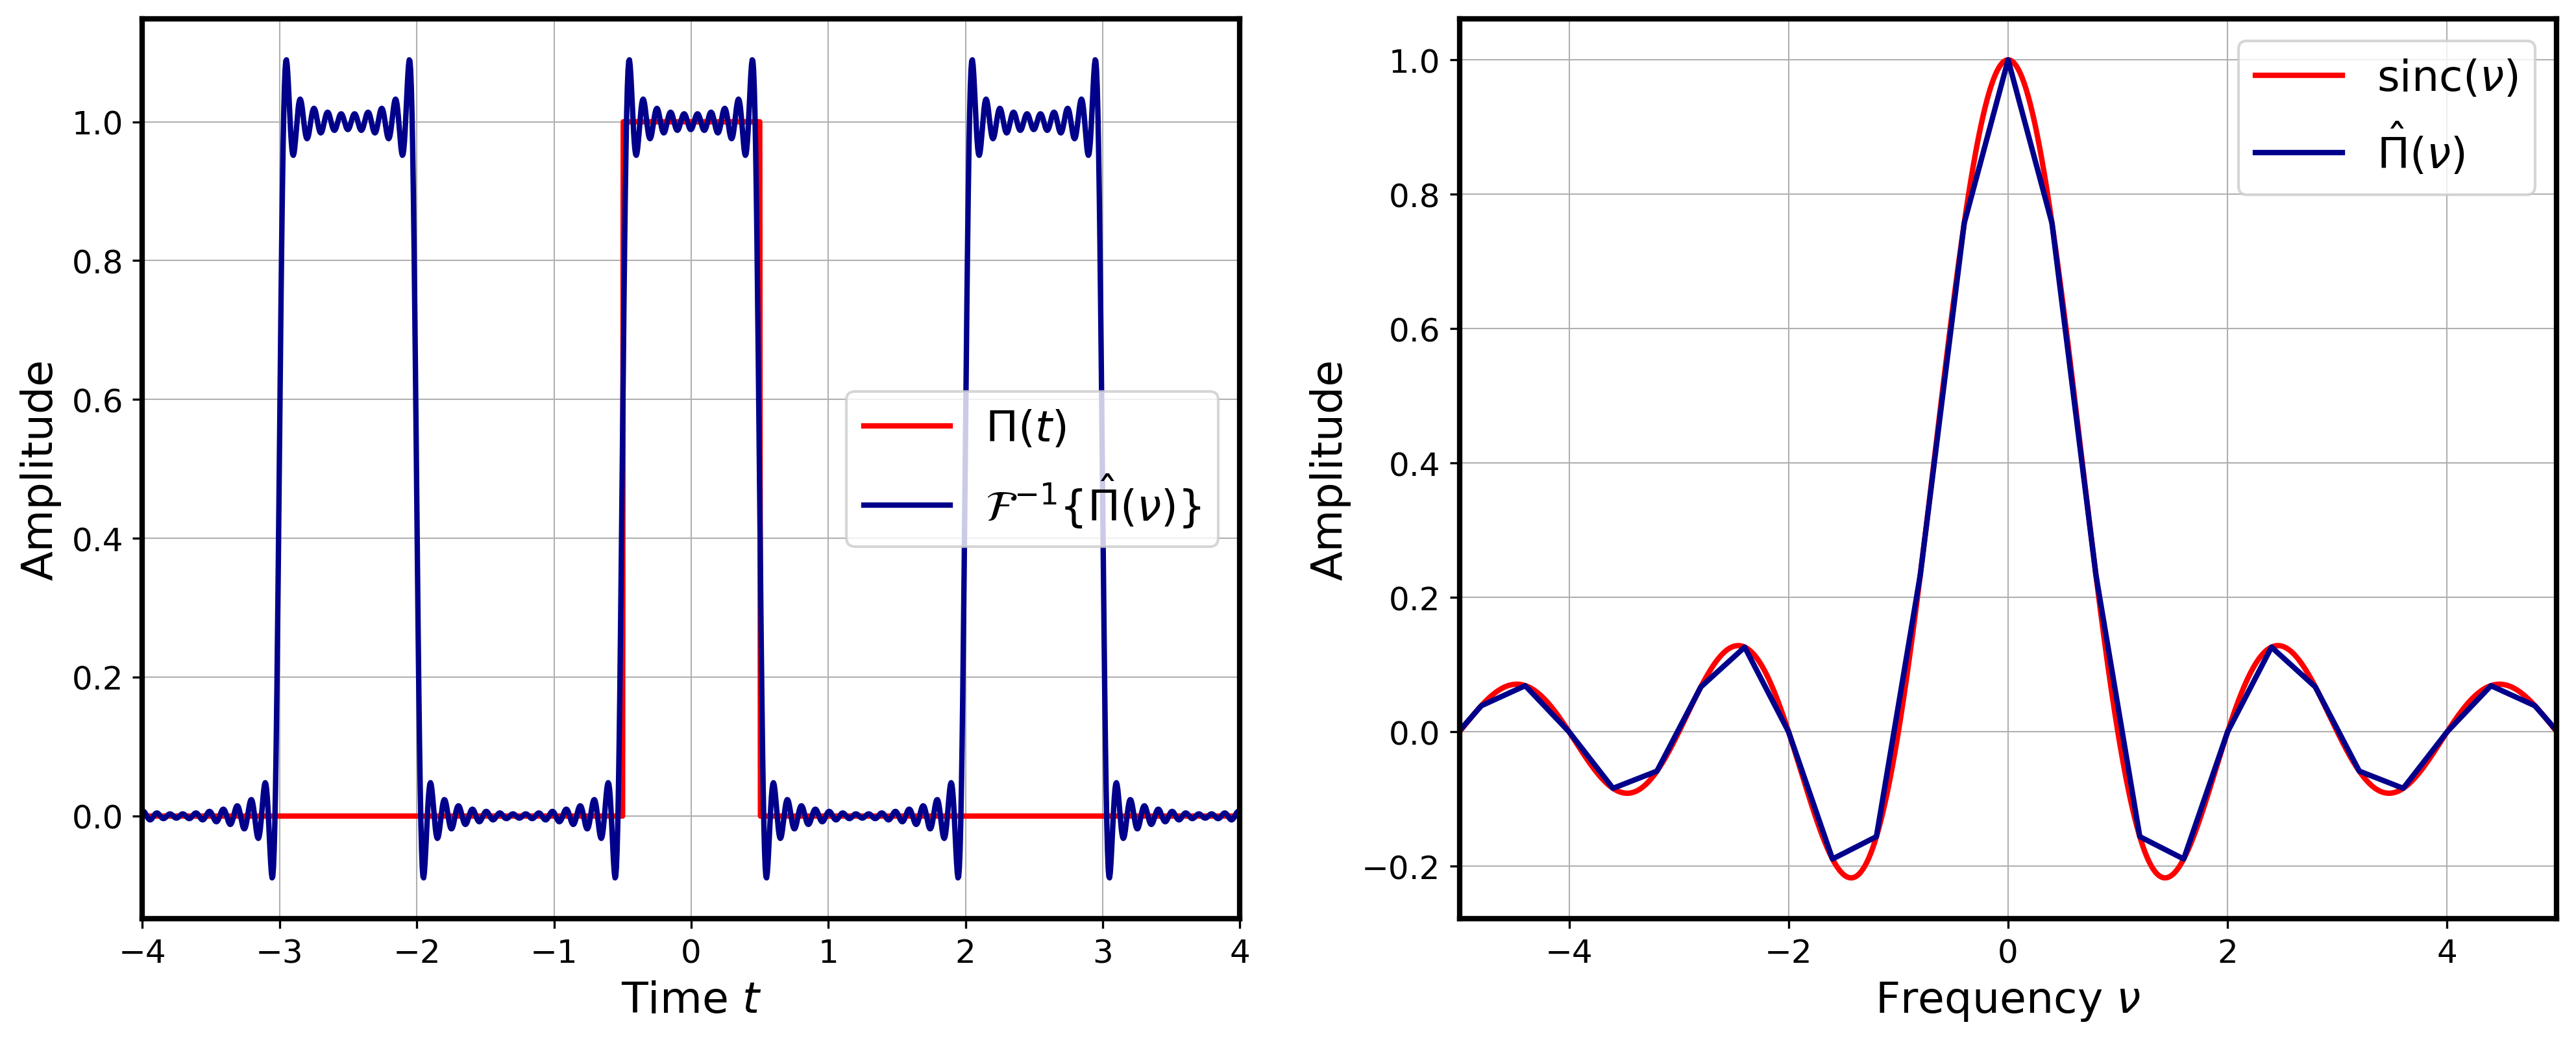
\includegraphics[width=1\textwidth]{../images/task1/combined_T_20_dt_0.005_V_20_dnu_0.4.png} 
	\caption{Графики функций и фурье-образов. \(\Delta \nu = 0.4\).}
\end{figure}


Время выполнения - 2.5 секунды.

\[\]

\textbf{Итог: } Увеличение шага по частоте снижает детализацию спектра, делая его более ступенчатым. Это сокращает время вычислений, но ухудшает восстановление сигнала - при \(\Delta \nu = 0.4\) у восстановленного сигнала наблюдается периодичность с периодом \(T = 2.5\).

\subsubsection{Вывод}

Численное интегрирование методом \texttt{trapz} показало свою эффективность для вычисления прямого и обратного преобразования Фурье прямоугольного импульса. Точность восстановления сигнала и его спектра зависит от выбора параметров:

\begin{itemize}

\item Параметры \(T\) и \(V\) определяют диапазоны по времени и частоте, при этом увеличение \(T\) не устраняет эффект Гиббса.


\item Шаг дискретизации \(\Delta t\) оказывает двоякое влияние: слишком малый шаг сохраняет эффект Гиббса, а слишком большой вызывает искажение амплитуды.

\item Шаг по частоте \(\Delta \nu\) влияет на детализацию спектра, при больших значениях возникает периодизация сигнала во временной области.

\end{itemize}

\newpage

\subsection{Использование DFT}

В этом задании мне нужно задать функцию \(\Pi(t)\), найти её Фурье-образ с помощью дискретного преобразования Фурье (конструкция \texttt{fftshift(fft())}), используя его так, чтобы преобразование было унитарным. Далее выполнить обратное преобразование от найденного Фурье-образа с помощью обратного дискретного преобразования (конструкция \texttt{ifft(ifftshift())}). Мои схематичные действия: 

\[
\Pi(t) \xrightarrow{\text{fftshift(fft())}} \hat{\Pi}(\nu) \xrightarrow{\text{ifft(ifftshift())}} \Pi(t)
\]

\textbf{Ожидаемые результаты}

\begin{itemize}
	\item Наиболее показательные значения параметров $T$, $\Delta t$, $V$, $\Delta \nu$.
	
	\item Графики аналитического образа и найденного с помощью DFT $\hat{\Pi}(\nu)$.
	
	\item Графики исходной $\Pi(t)$ и восстановленных функций.
	
	\item Выводы о влиянии шага и промежутка интегрирования и о точности и быстродействии метода.
	
\end{itemize}
\hrule

\subsubsection{Предподготовка}

Задам функцию \(\Pi(t)\) в python. Зафиксирую параметры функции $T = 20$, $\Delta t = 0.005$. Отрисую полученные сигналы и образы.
\begin{figure}[h]
	\centering
	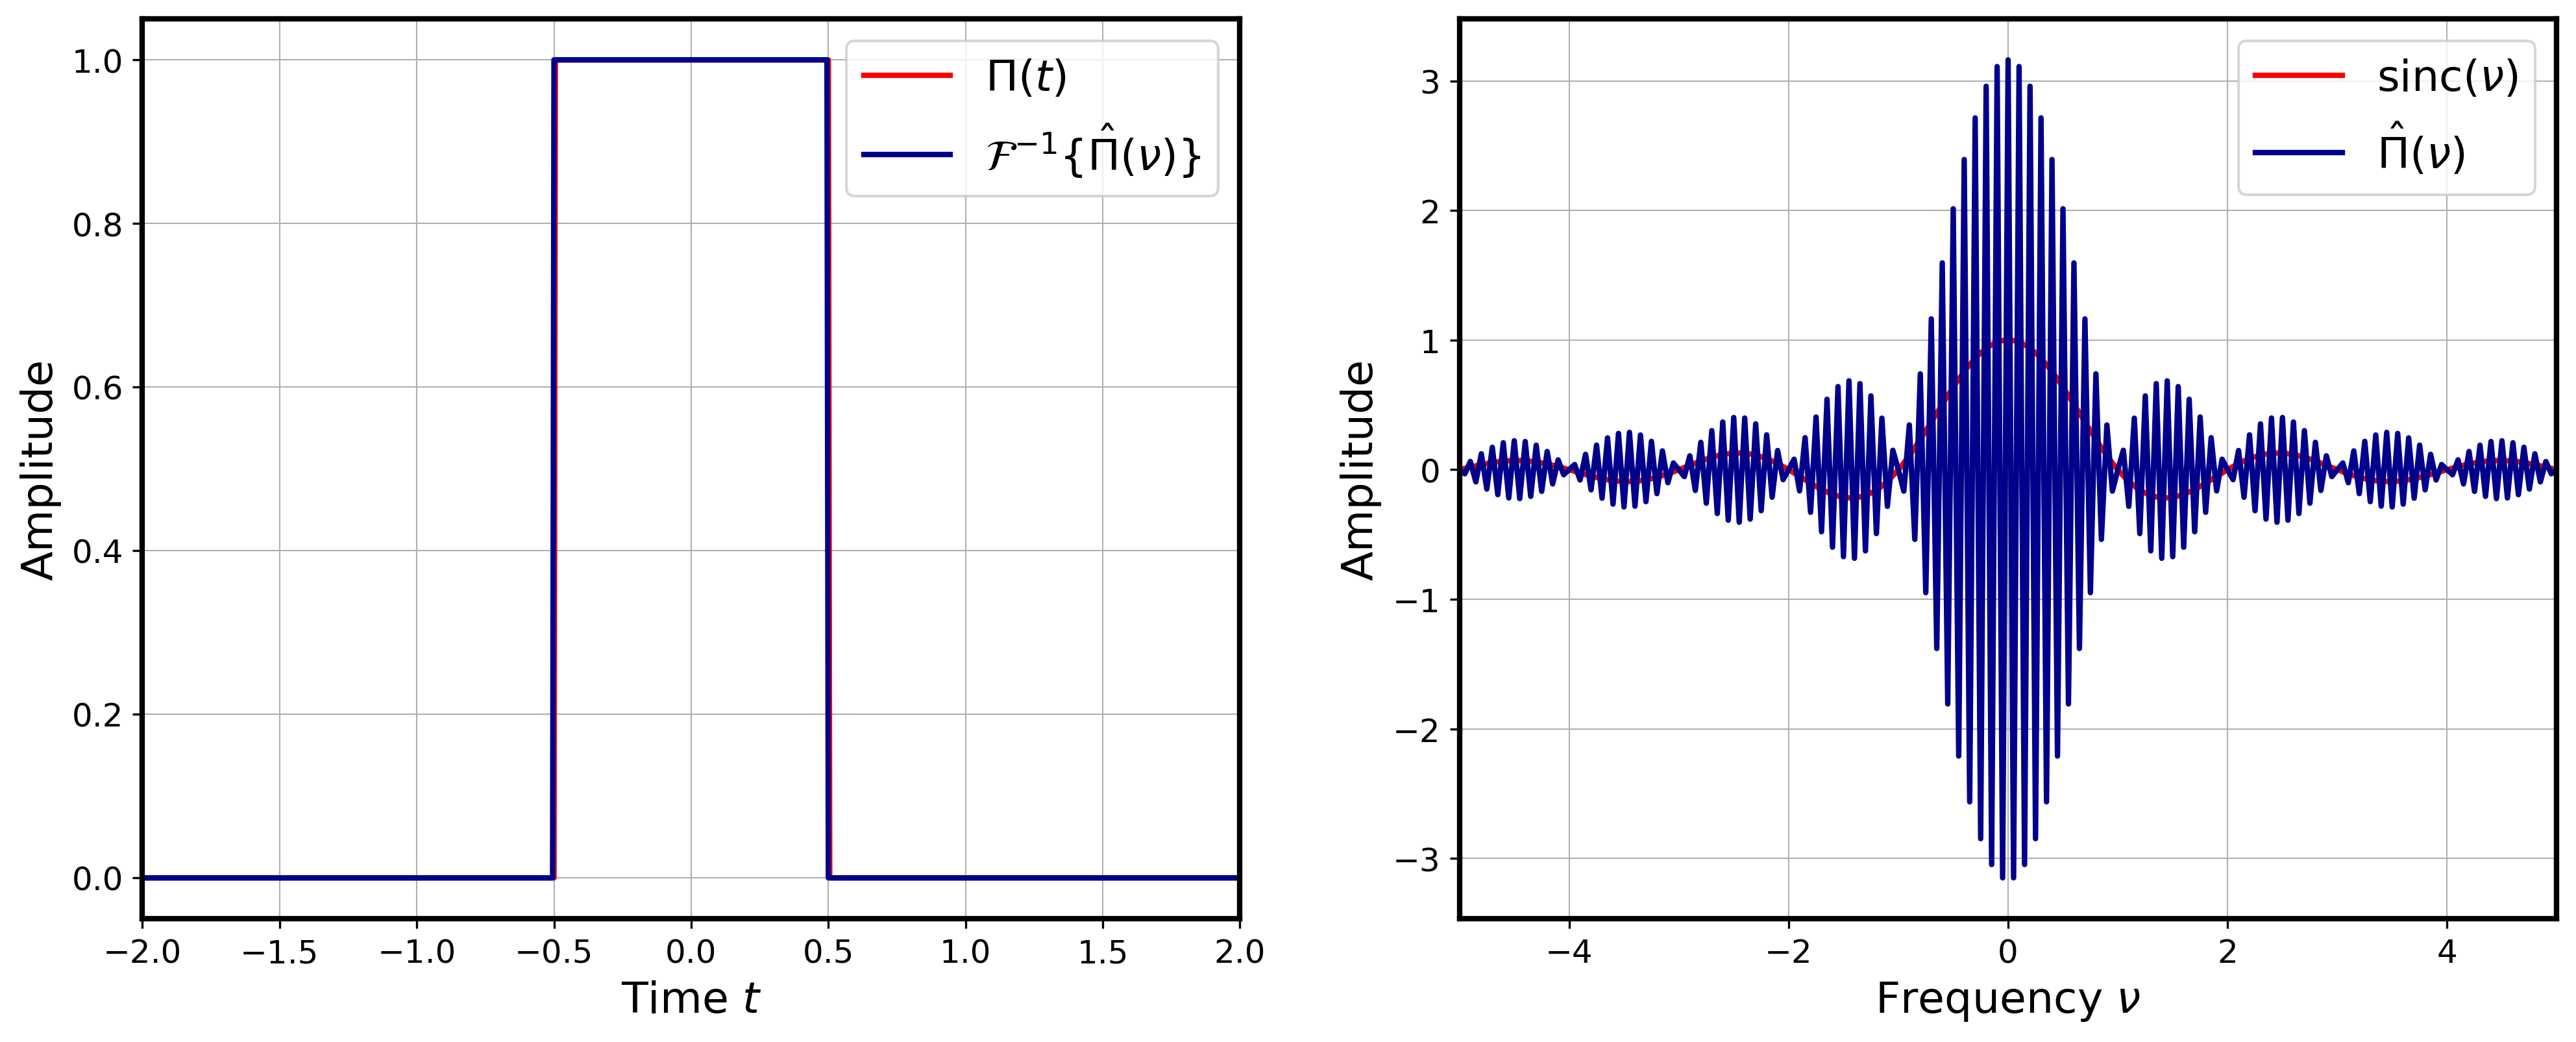
\includegraphics[width=1\textwidth]{../images/task2/combined_T_20_dt_0.005.png} 
	\caption{График функции и фурье-образа.}
\end{figure}

\subsubsection{Влияние параметра \(T\)}

Зафиксирую \(\Delta t = 0.005\). Возьму значения \(T \in [40, 10, 1]\) и посмотрю на изменения. Сравню время выполнения цикла со временем выполнения цикла из предыдущего пункта ~\ref{subsec:trapz}.



\begin{figure}[H]
	\centering
	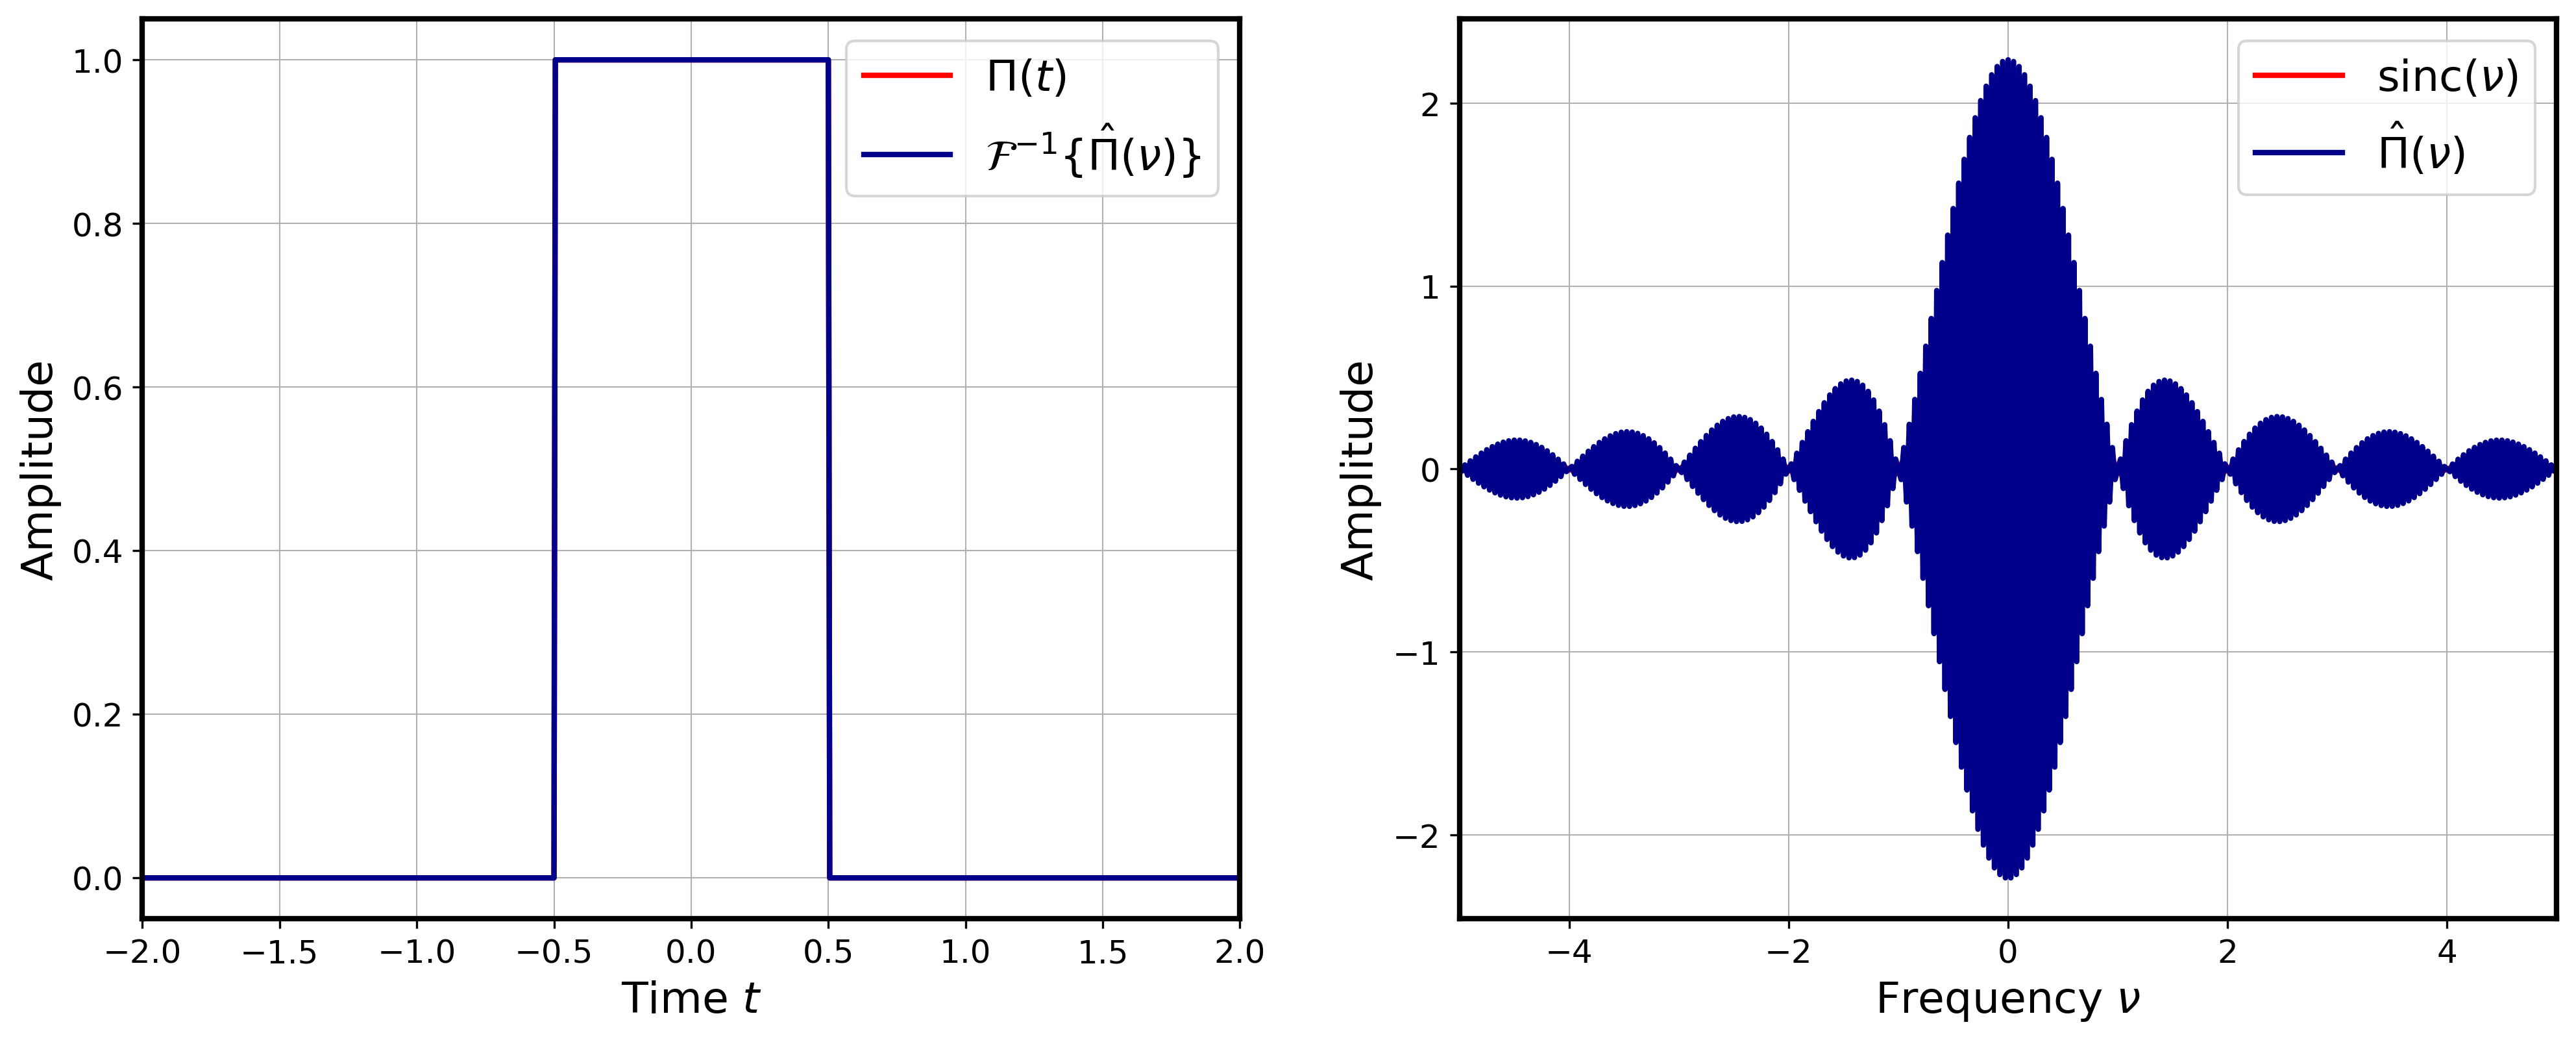
\includegraphics[width=1\textwidth]{../images/task2/combined_T_40_dt_0.005.png} 
	\caption{Графики функций и фурье-образов. \(T = 40\).}
\end{figure}


\begin{figure}[H]
	\centering
	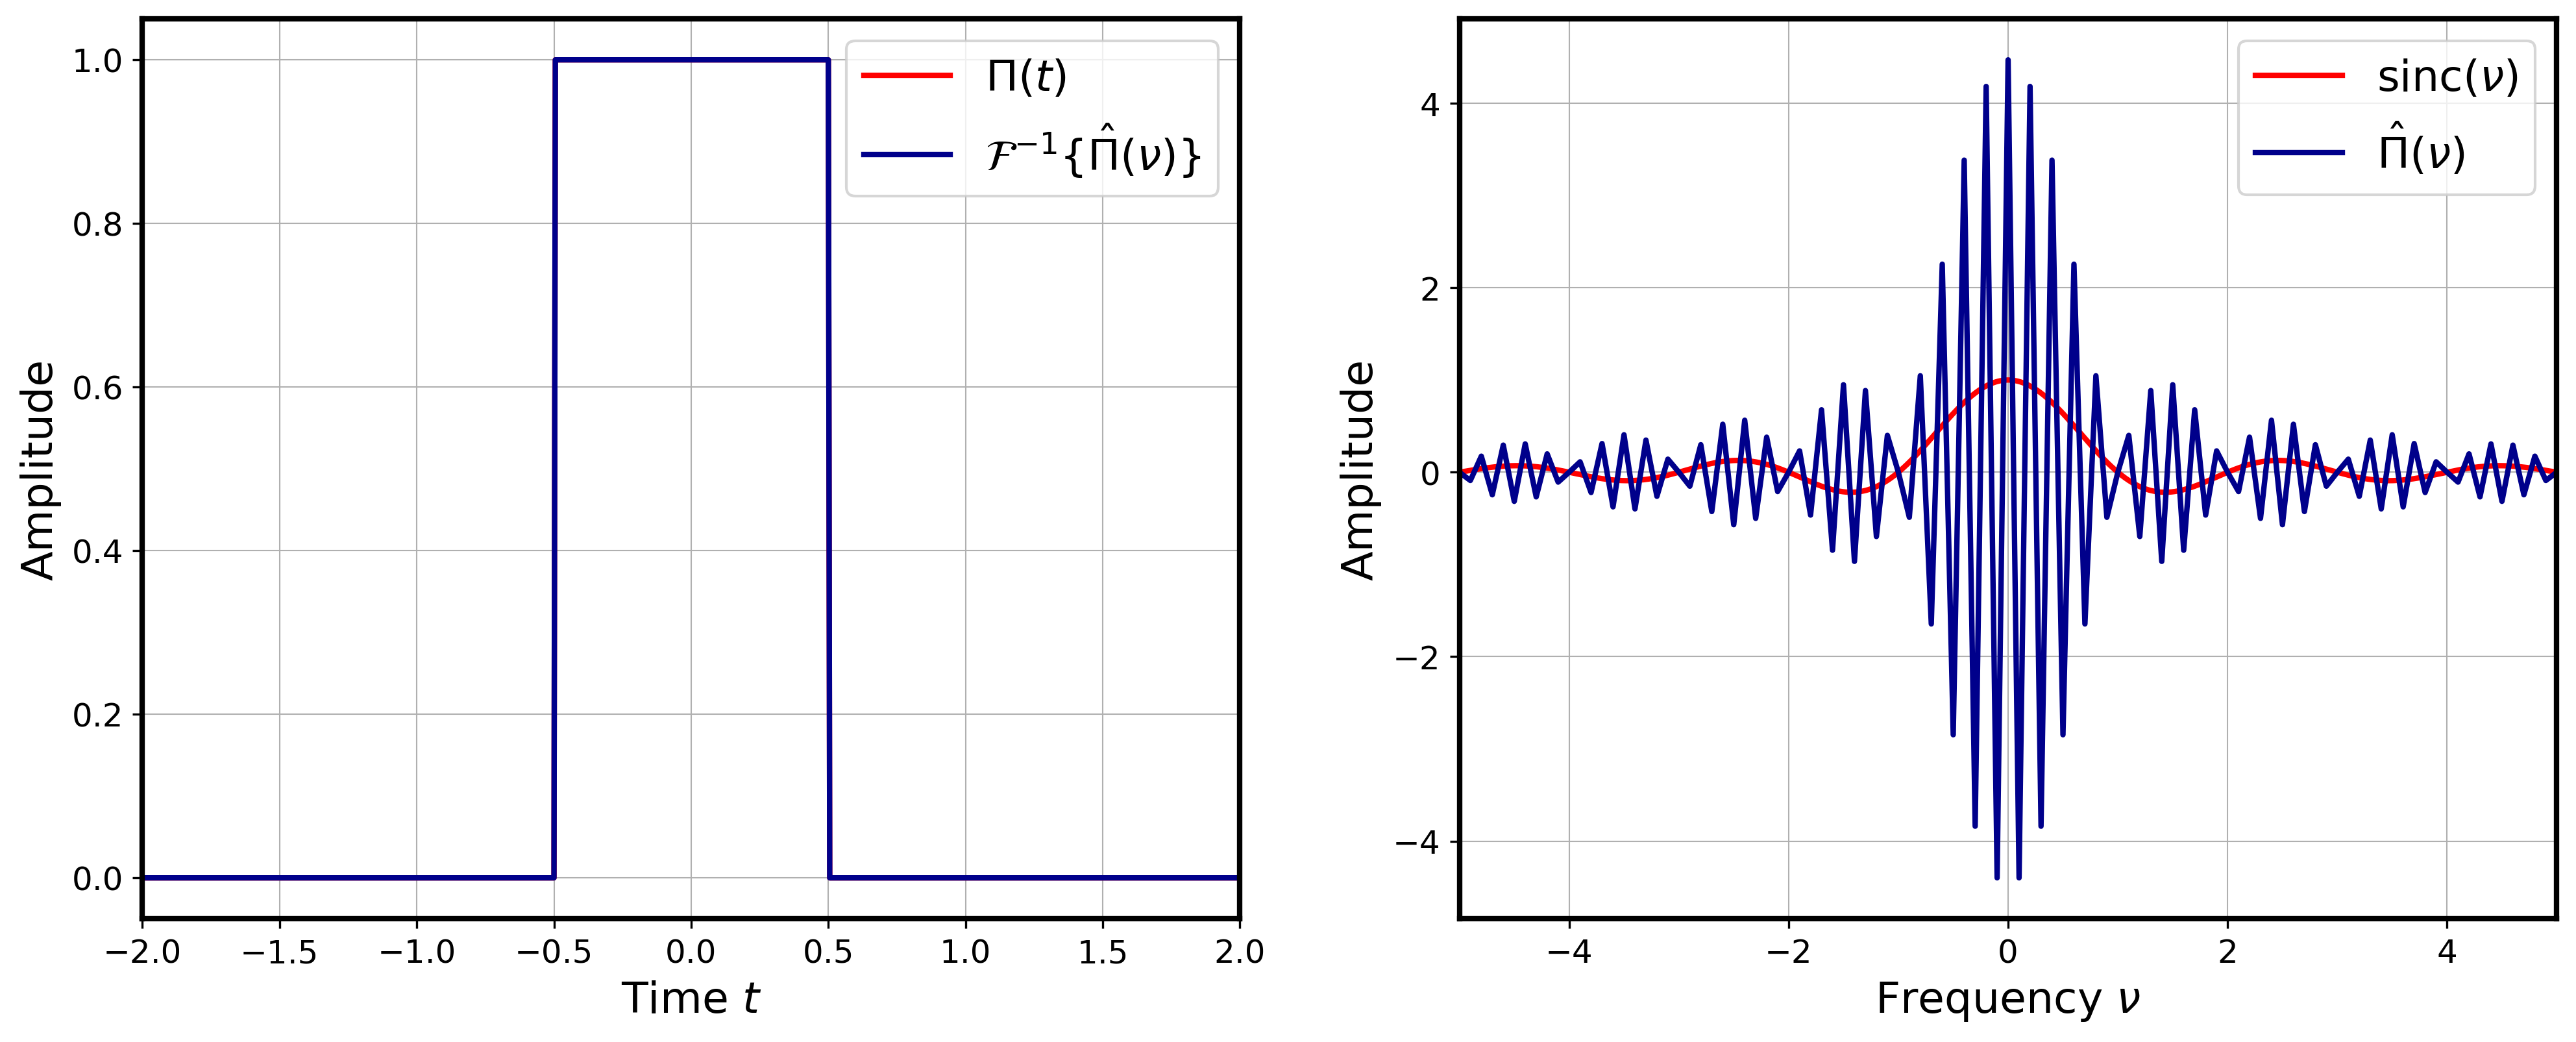
\includegraphics[width=1\textwidth]{../images/task2/combined_T_10_dt_0.005.png} 
	\caption{Графики функций и фурье-образов. \(T = 10\).}
\end{figure}



\begin{figure}[H]
	\centering
	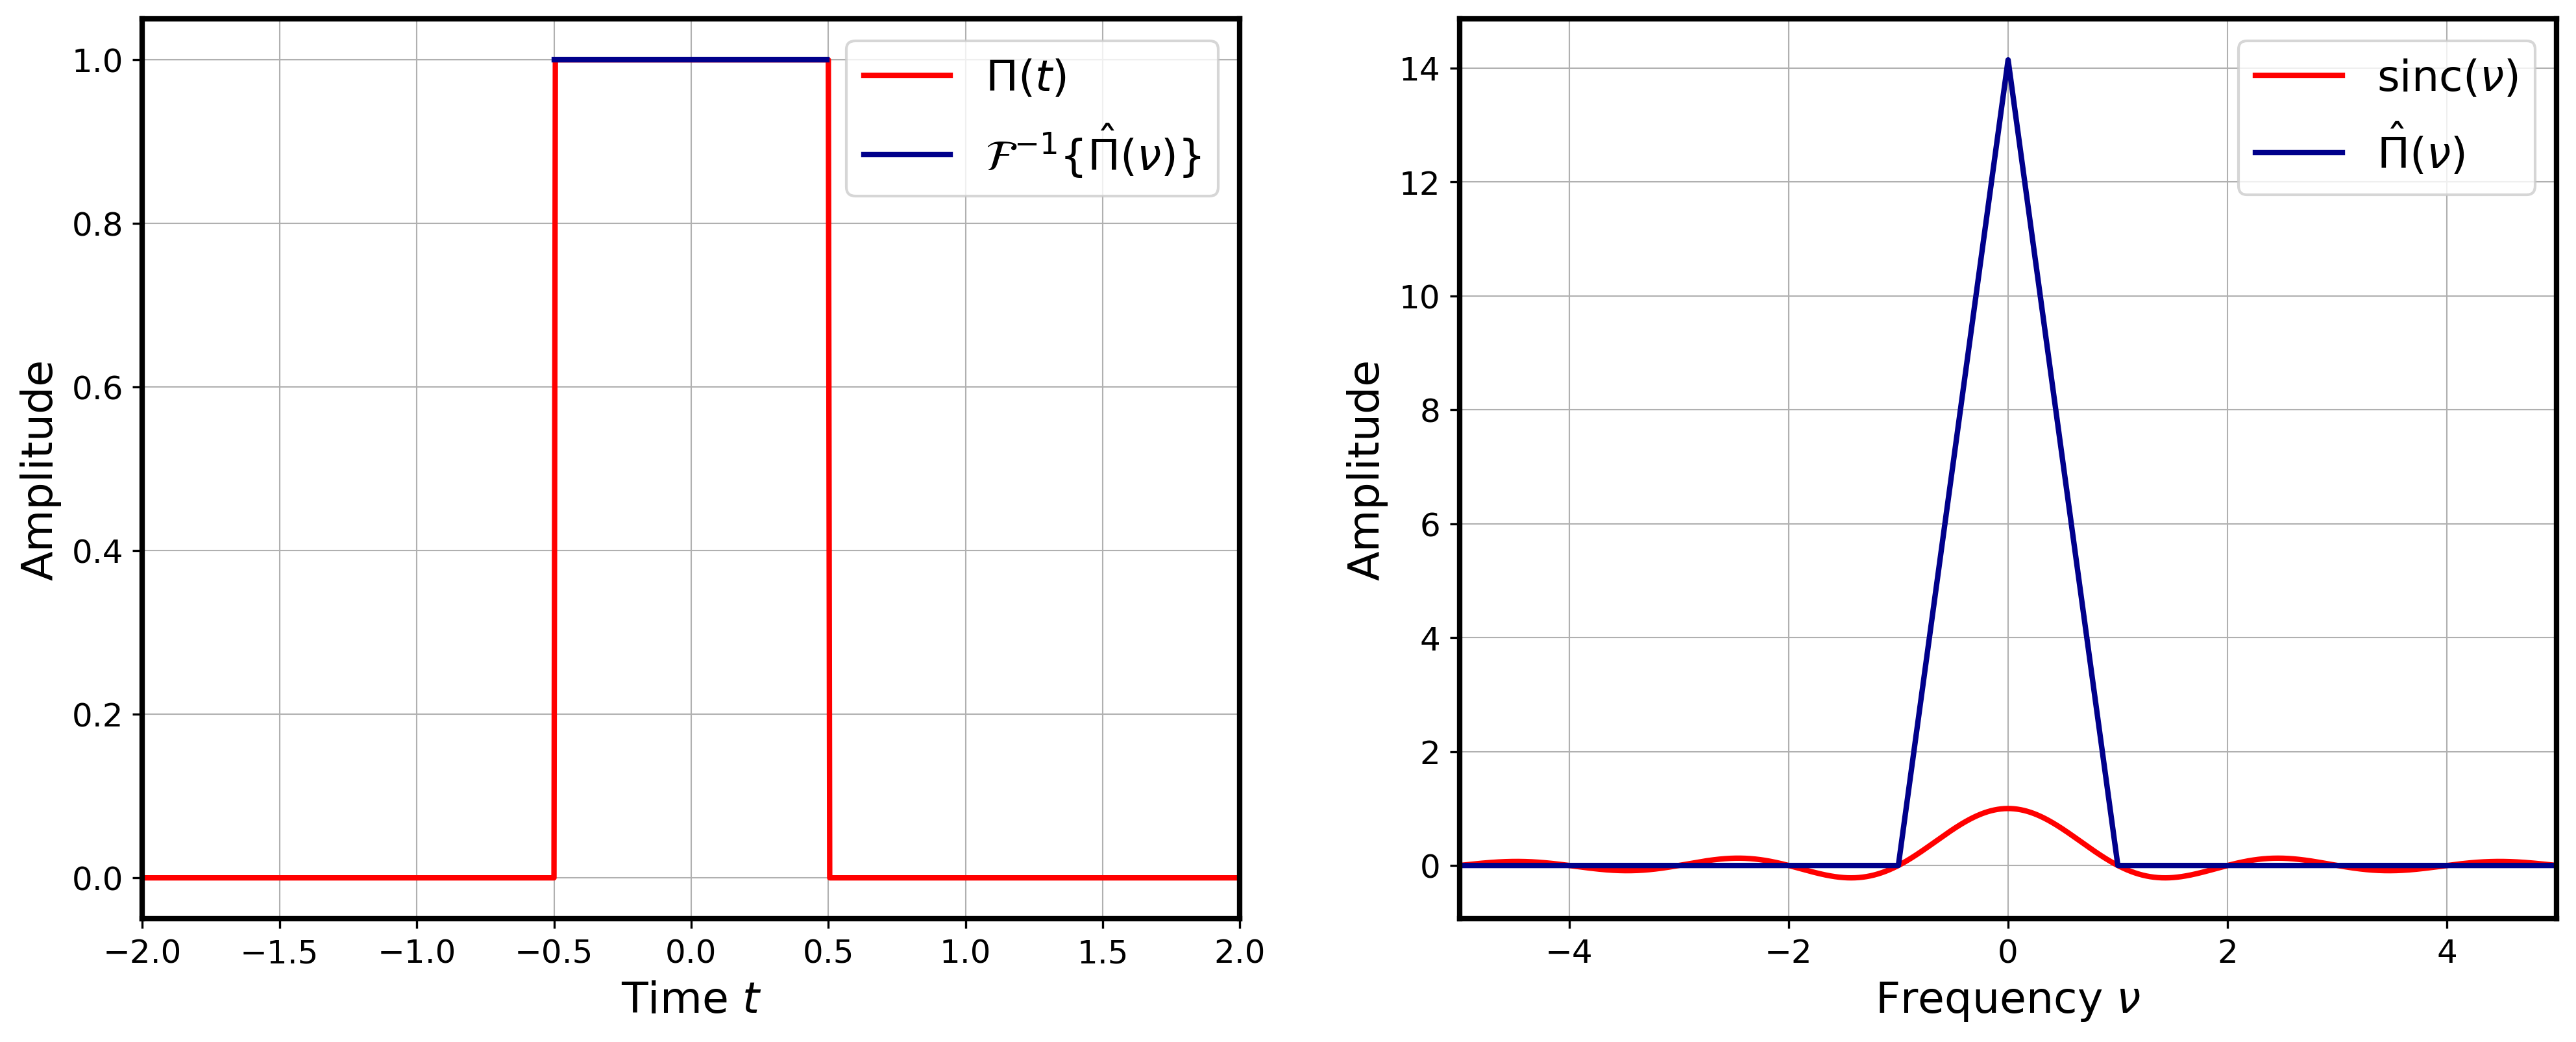
\includegraphics[width=1\textwidth]{../images/task2/combined_T_1_dt_0.005.png} 
	\caption{Графики функций и фурье-образов. \(T = 1\).}
\end{figure}



\[\]


\textbf{Итог: } Восстановление сигнала при \(T = 40\) и \(T = 10\) схоже. Уменьшение параметра давало очень хорошее восстановление сигнала без эффекта Гиббса. Однако фурье-образы сигналов различаются в частотной области. Время выполнения циклов уменьшилось - \texttt{FFT} работает быстрее. Метод работает гораздо быстрее предыдущего - расчеты занимают не более секунды.

\subsubsection{Влияние параметра \(\Delta t\)}

Зафиксирую \(T = 20\). Возьму значения \(T \in [0.01, 0.1, 0.4]\) и посмотрю на изменения. Сравню время выполнения цикла со временем выполнения цикла из предыдущего пункта ~\ref{subsec:trapz}.

\begin{figure}[H]
	\centering
	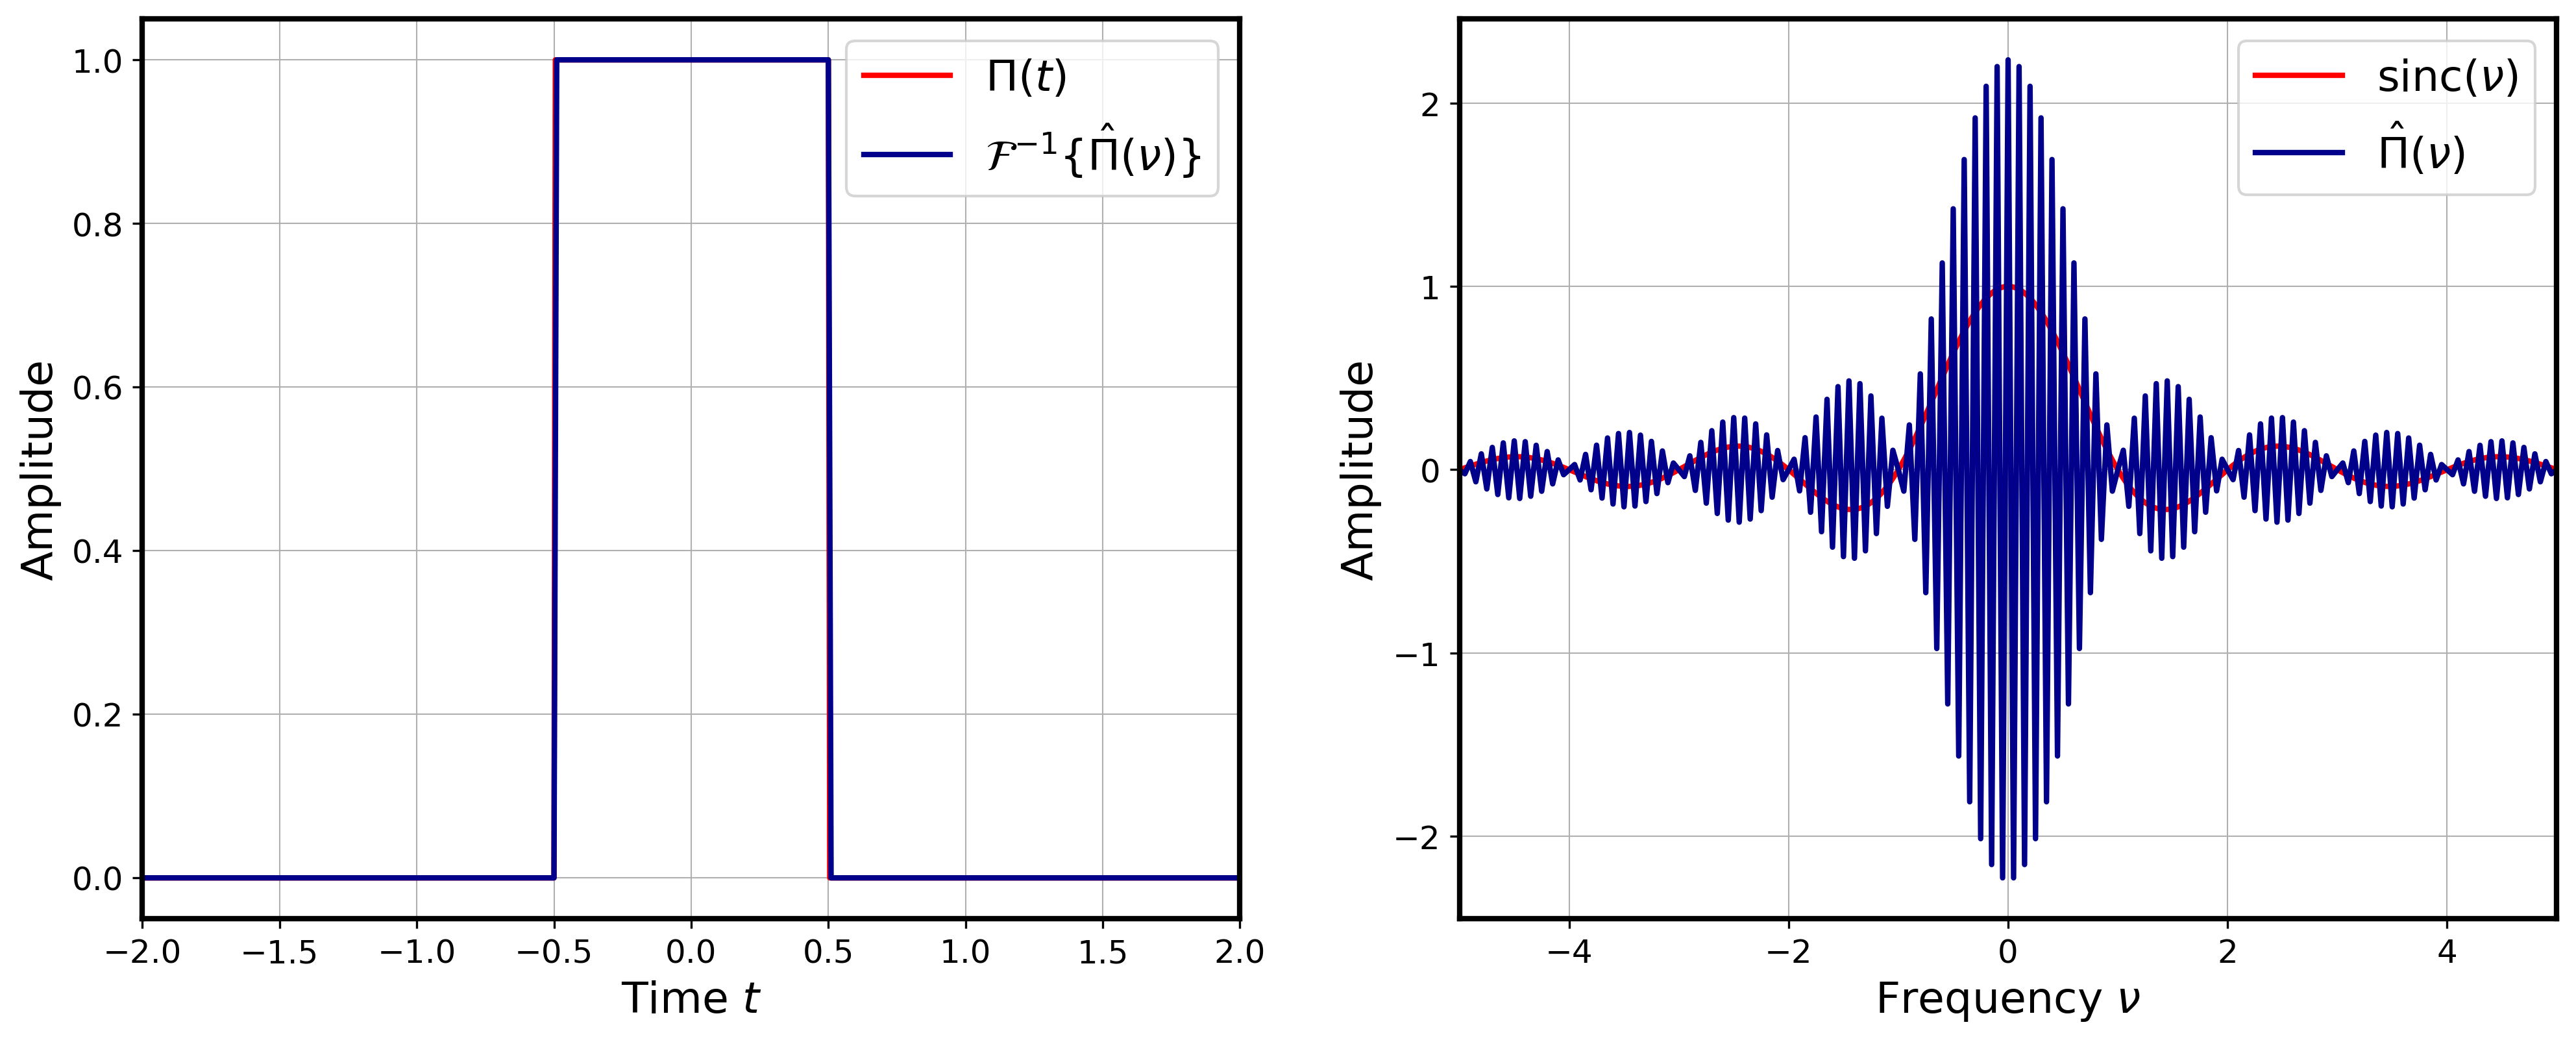
\includegraphics[width=1\textwidth]{../images/task2/combined_T_20_dt_0.01.png} 
	\caption{Графики функций и фурье-образов. \(\Delta t = 0.01\).}
\end{figure}


\begin{figure}[H]
	\centering
	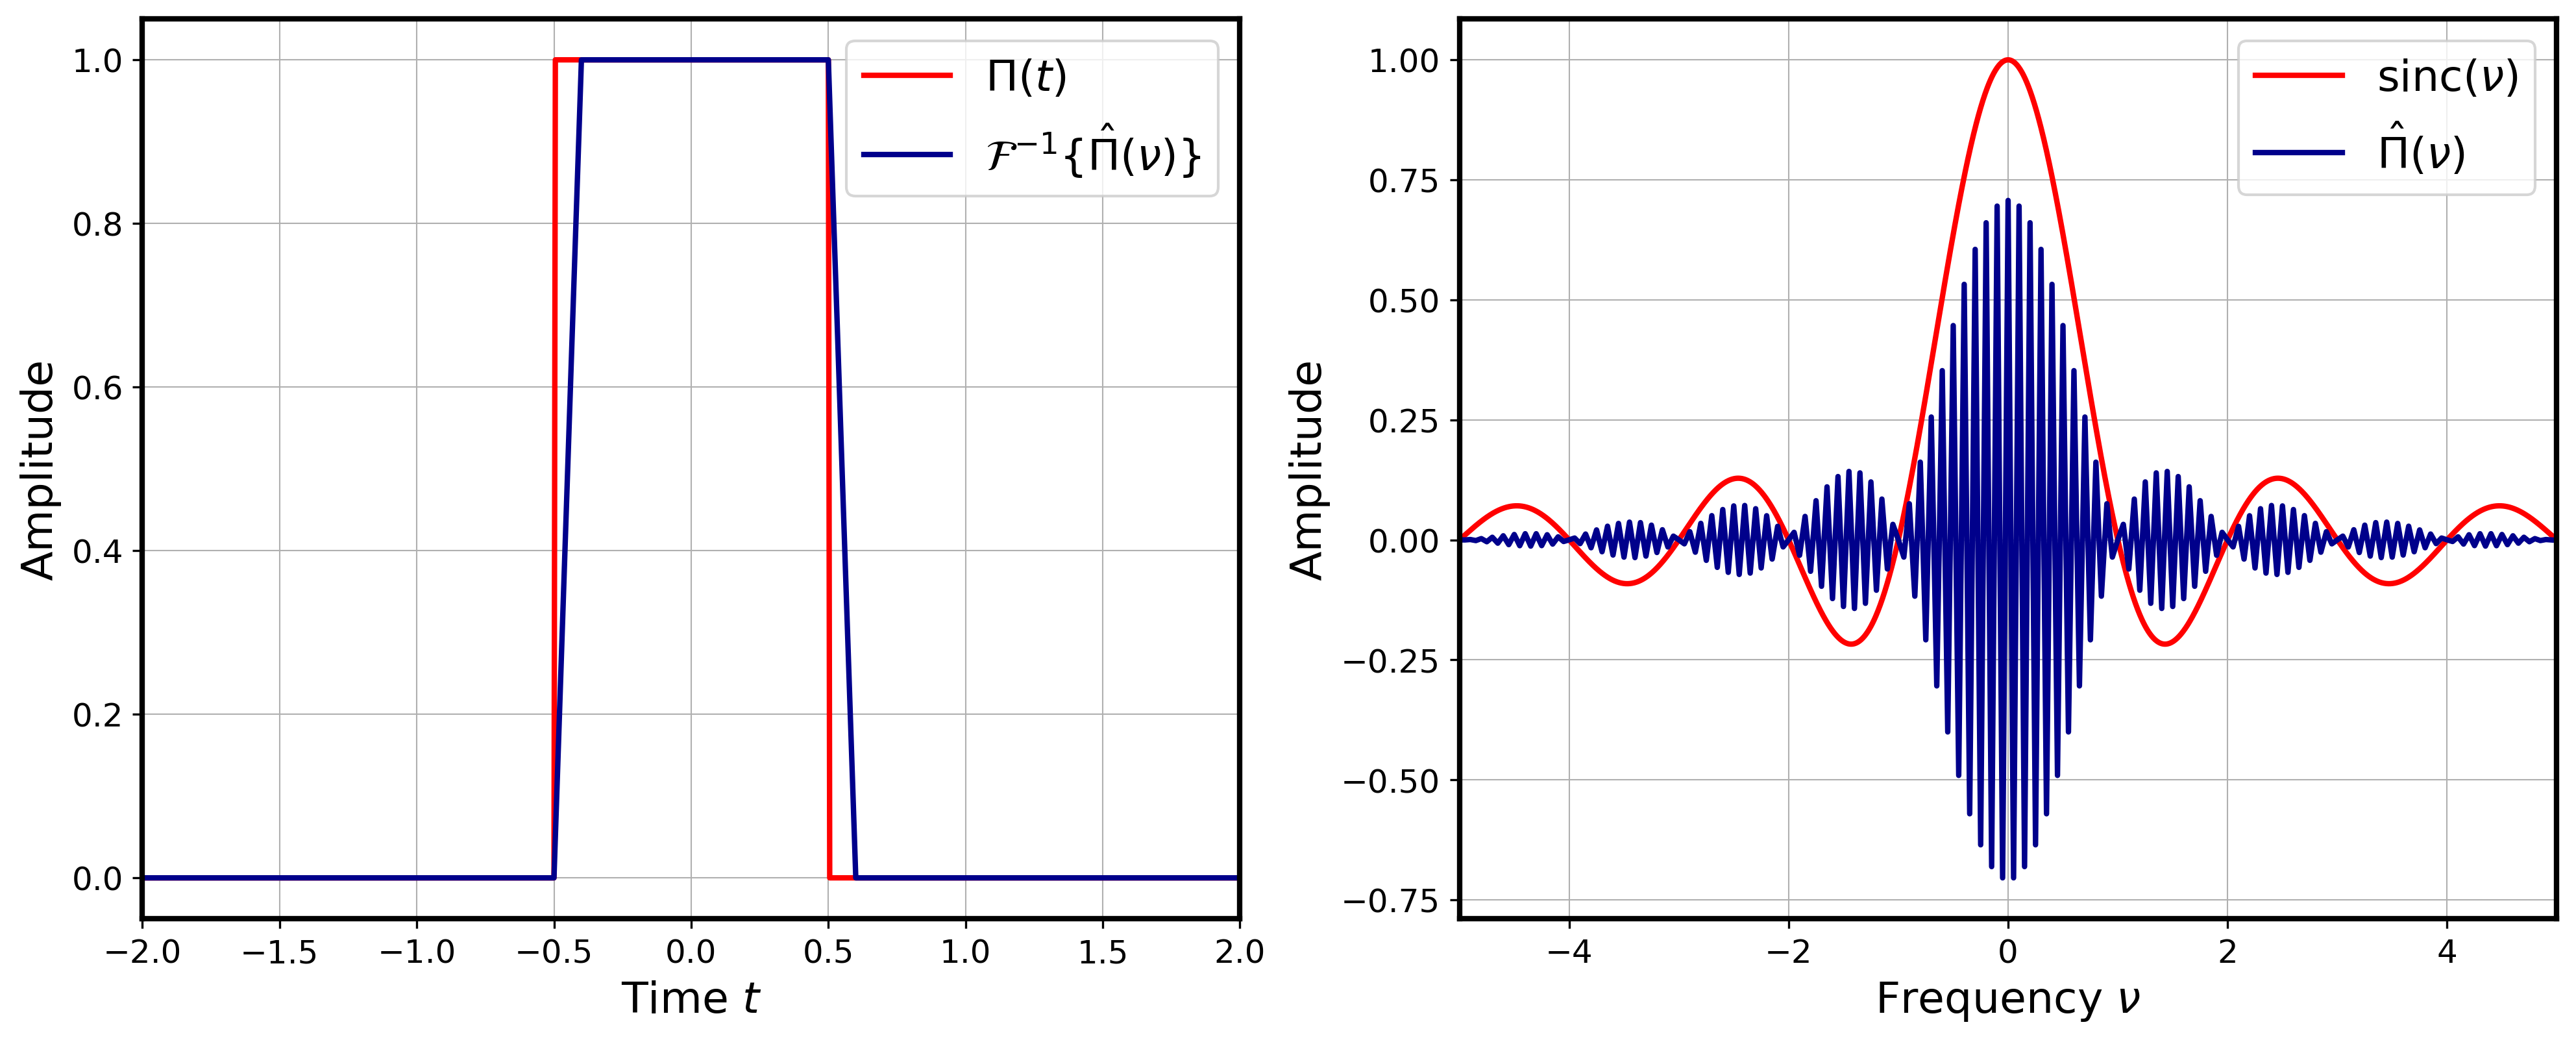
\includegraphics[width=1\textwidth]{../images/task2/combined_T_20_dt_0.1.png} 
	\caption{Графики функций и фурье-образов. \(\Delta t = 0.1\).}
\end{figure}


\begin{figure}[H]
	\centering
	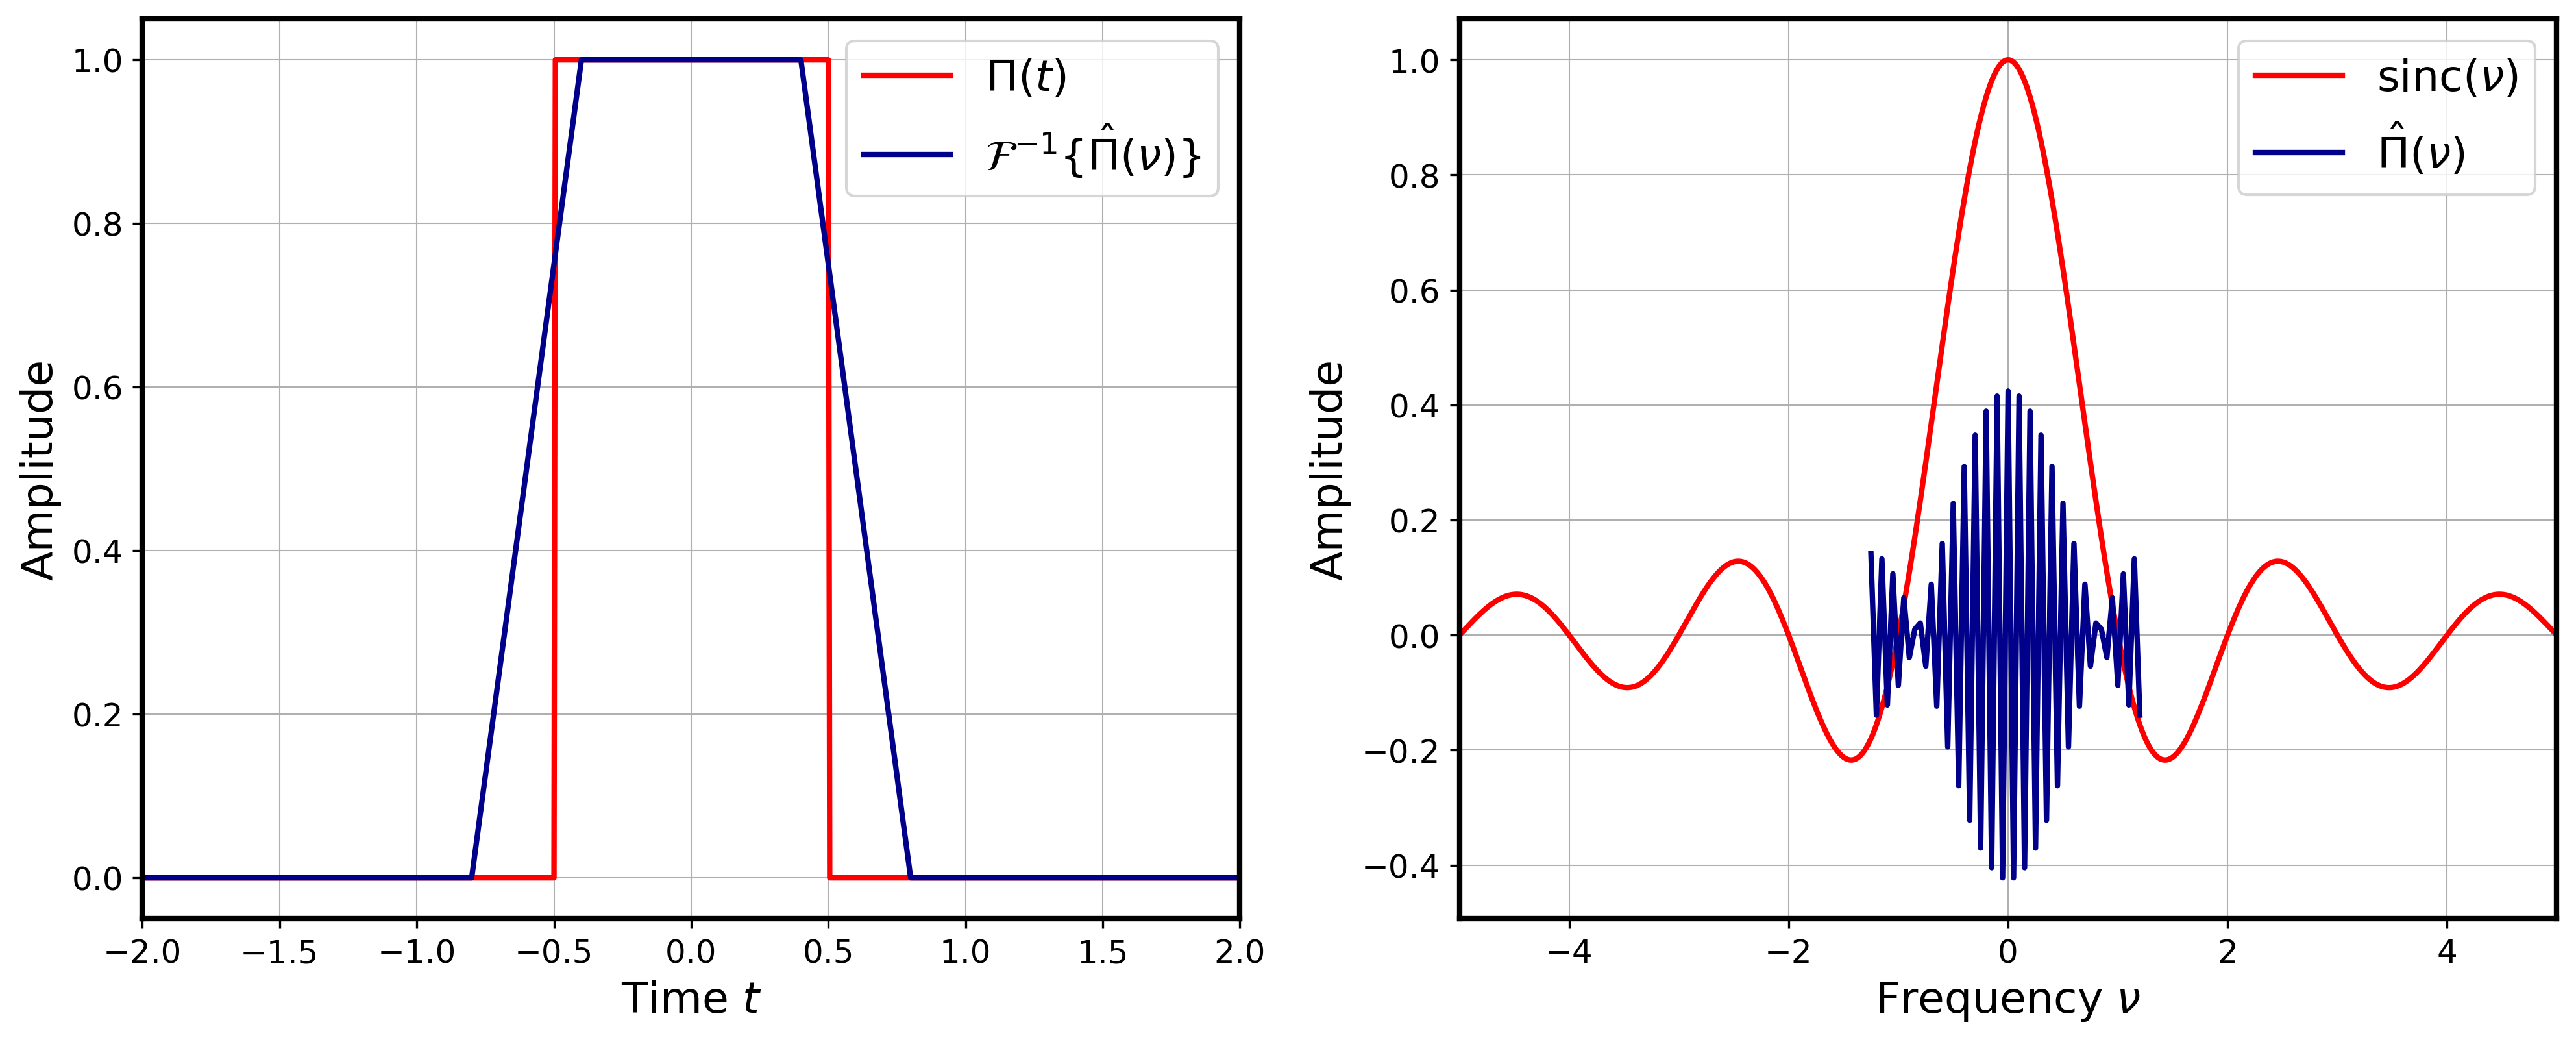
\includegraphics[width=1\textwidth]{../images/task2/combined_T_20_dt_0.4.png} 
	\caption{Графики функций и фурье-образов. \(\Delta t = 0.4\).}
\end{figure}



\[\]


\textbf{Итог: } Увеличение параметра \(\Delta t\) приводит к неточной реконструкции сигнала. Однако при использовании метода \texttt{FFT} не наблюдается искажение сигнала по амплитуде. Метод также сработал быстрее, чем \texttt{trapz}.


\subsubsection{Вывод}

Метод дискретного преобразования Фурье продемонстрировал существенные преимущества перед численным интегрированием по быстродействию, сократив время вычислений в 2-3 раза при сохранении точности. Анализ влияния параметров показал, что:

\begin{itemize}
	\item Параметр \(T\) оказывает значительное влияние на частотное разрешение - при малых значениях (\(T = 1\)) наблюдается неточный спектр.
	\item Параметр \(\Delta t\) важен для точности реконструкции - увеличение шага дискретизации свыше 0.1 приводит к искажениям сигнала, но не приводит к изменениям амплитуды сигнала.
\end{itemize}

\newpage

\subsection{Объяснения}

\begin{itemize}
	
	\item Метод \texttt{trapz}
	
	Основан на численном интегрировании по формуле трапеций:
	\[
	\int_a^b f(x)dx \approx \frac{b-a}{2N}\sum_{n=1}^N (f(x_n) + f(x_{n+1}))
	\]
	
	Данный метод аппроксимирует непрерывное преобразование Фурье, вычисляя интеграл на произвольной сетке частот. Это обеспечивает высокую точность соответствия аналитическому решению (функции $\mathrm{sinc}(\nu)$), но требует значительных вычислительных ресурсов из-за сложности $O(N^2)$.
	
	\item Метод \texttt{FFT}
	
	Реализует дискретное преобразование Фурье:
	\[
	X_k = \sum_{n=0}^{N-1} x_n \cdot e^{-2\pi i kn/N}
	\]
	
	Алгоритм использует симметрию комплексных экспонент, что снижает сложность до $O(N\log N)$. 
\end{itemize}

Метод \texttt{trapz} обеспечивает лучшее приближение к теоретическому спектру благодаря непрерывной аппроксимации, но требует больших вычислительных затрат. Метод \texttt{FFT}, хотя и дает менее точный спектр, обеспечивает высокую скорость вычислений и точное обратное преобразование.

\newpage

\subsection{Приближение непрерывного с помощью DFT}

Требуется совместить преимущества методов \texttt{trapz} (точность) и \texttt{FFT} (быстродействие) для вычисления непрерывного преобразования Фурье. Схема решения:

\[
\Pi(t) \xrightarrow{\text{умное использование FFT}} \hat{\Pi}(\nu) \xrightarrow{\text{умное использование IFFT}} \Pi(t)
\]


\textbf{Ожидаемые результаты}

\begin{itemize}
	\item Аналитический вывод коэффициентов $c_m$
	\item Исследование метода для различных $T$ и $\Delta t$
	\item Сравнительные графики с аналитическим решением
	\item Сравнение с методами \texttt{trapz} и стандартным \texttt{FFT}
	\item Анализ точности и быстродействия
\end{itemize}

\hrule

\subsubsection{Предподготовка}

Для аппроксимации непрерывного преобразования Фурье на конечном промежутке $[a, b]$ используется дискретная сумма Римана:

\[
\hat{f}(\nu_m) \approx \sum_{n=0}^{N-1} f(t_n) \, e^{-2\pi i \nu_m t_n} \, \Delta t,
\]

где:
\begin{itemize}
	\item $t_n = a + n \Delta t$ — точки дискретизации по времени;
	\item $\Delta t = \dfrac{b - a}{N - 1}$ — шаг дискретизации;
	\item $\nu_m$ — частоты, на которых вычисляется преобразование.
\end{itemize}

Данное выражение можно привести к форме дискретного преобразования Фурье с соответствующим масштабирующим коэффициентом:

\[
\hat{f}(\nu_m) \approx c_m \cdot \mathrm{DFT}(f)_m = c_m \, \sum_{n=0}^{N-1} f(t_n) \, e^{\frac{-2\pi i m n}{N}}.
\]

Сравнивая два выражения, находим коэффициент $c_m$:

\[
c_m = \Delta t \cdot e^{-2\pi i \nu_m a}.
\]

Для обратного преобразования и точного восстановления исходной функции используется коэффициент, обратный к $c_m$:

\[
c_m^{-1} = \frac{1}{\Delta t} \cdot e^{2\pi i \nu_m a}.
\]

Таким образом, предложенный подход позволяет эффективно сочетать вычислительную производительность алгоритма быстрого преобразования Фурье с точностью, соответствующей непрерывному интегральному преобразованию.

\subsubsection{Влияние параметра \(T\)}

Зафиксирую \(\Delta t = 0.005\). Возьму значения \(T \in [40, 10, 1]\) и посмотрю на изменения. Для каждого \(T\) расчитаю параметр частоты дискретизации по формуле \[\Delta \nu = \frac{1}{T}\] А для фиксированного значения \(\Delta t = 0.005\) можно расчитать длину частотного диапазона по формуле \[V = \frac{1}{\Delta t} = \frac{1}{0.005} = 200\]

\begin{figure}[H]
	\centering
	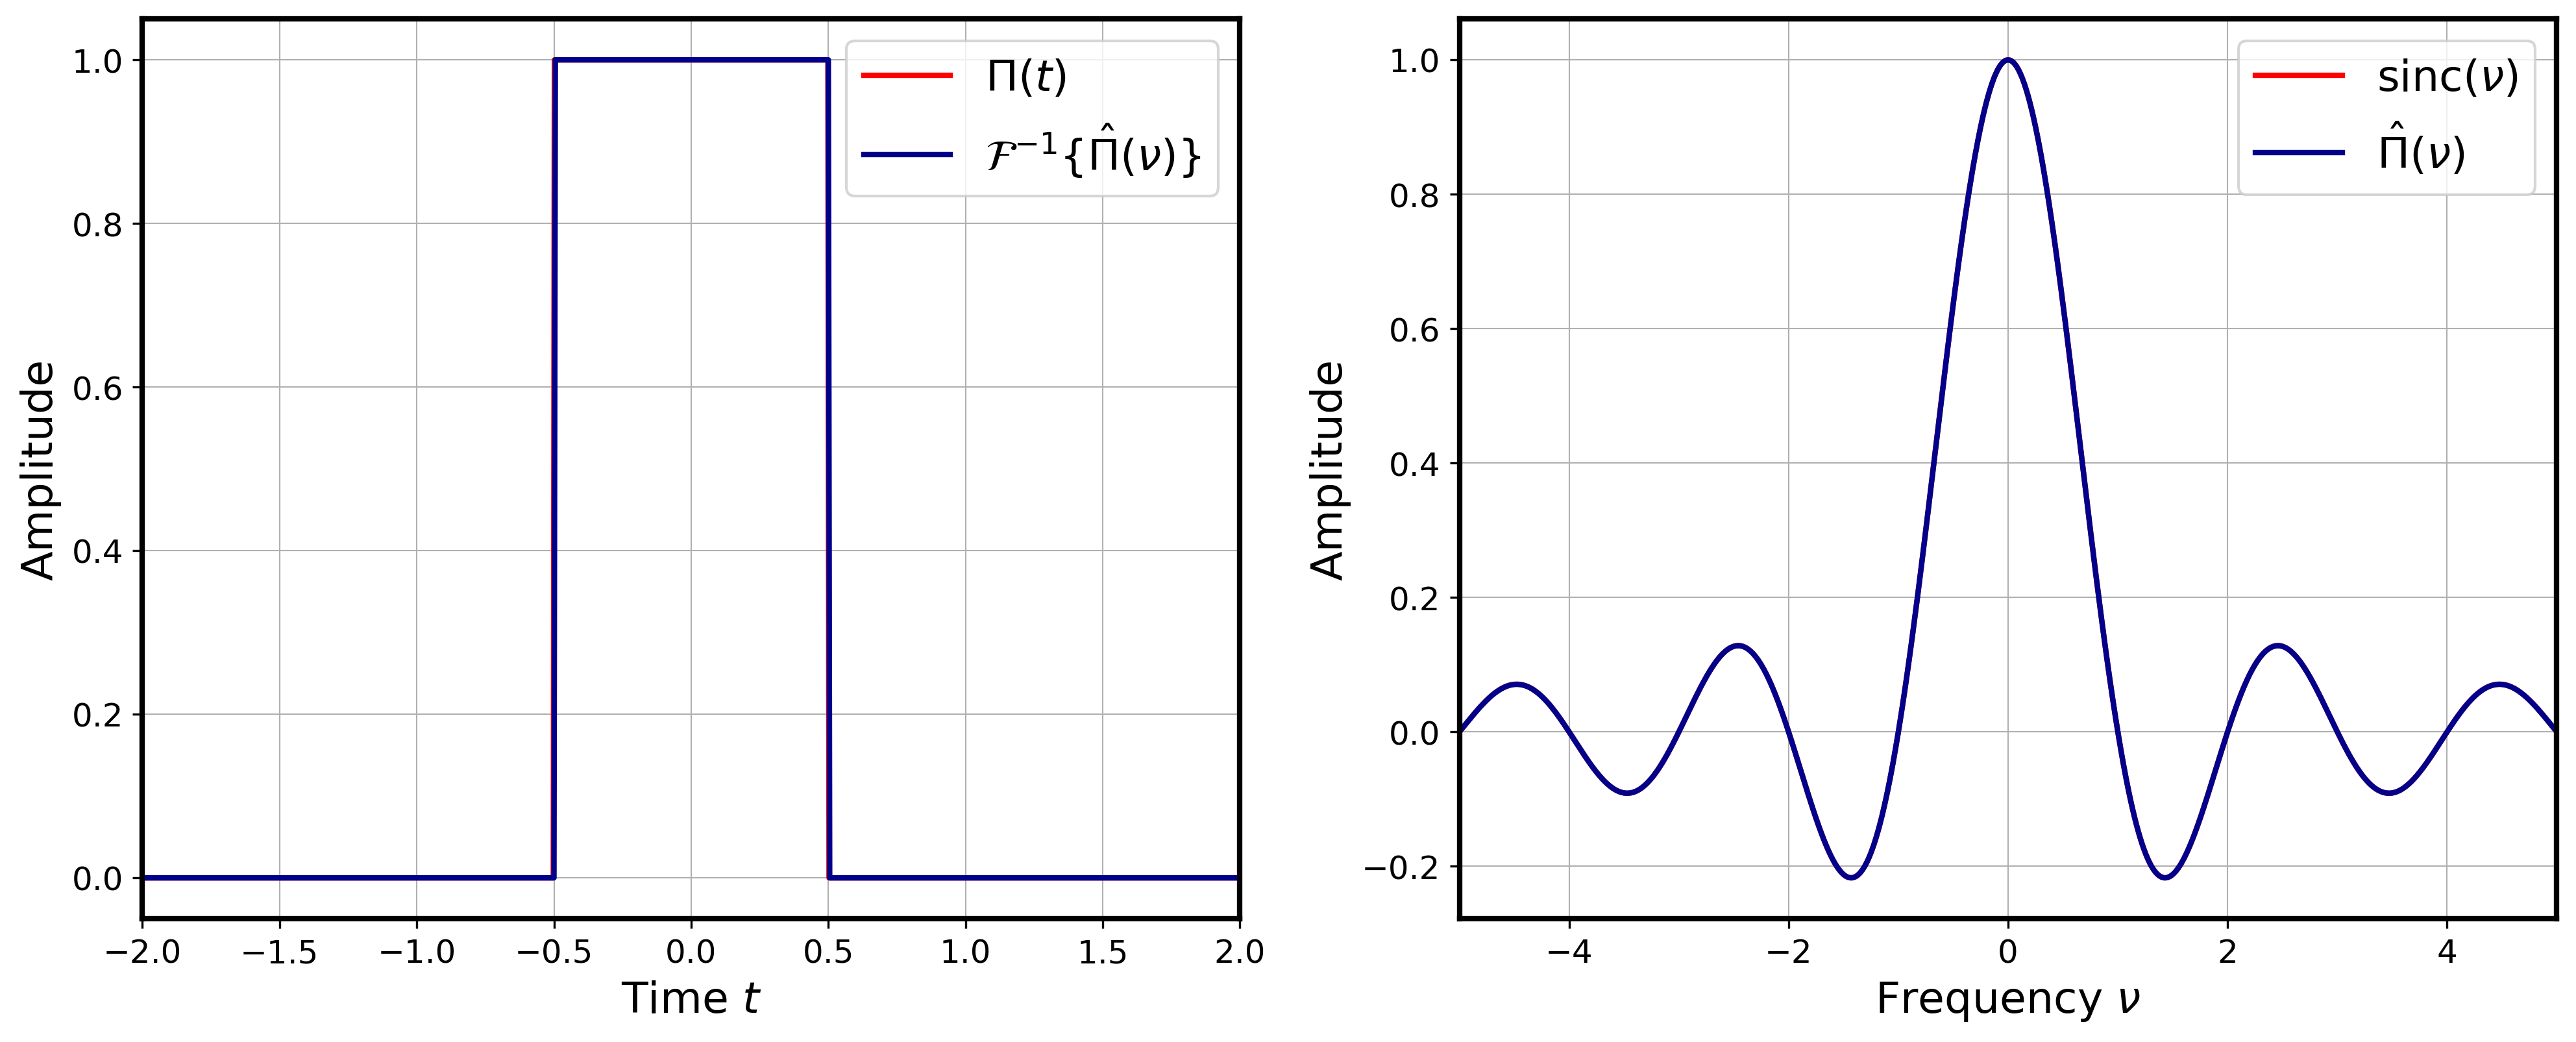
\includegraphics[width=1\textwidth]{../images/task3/continuous_T_40_dt_0.005.png} 
	\caption{Графики функций и фурье-образов. \(T = 40\).}
\end{figure}

Частота дискретизации \[\Delta \nu = \frac{1}{40} = 0.025\]

\begin{figure}[H]
	\centering
	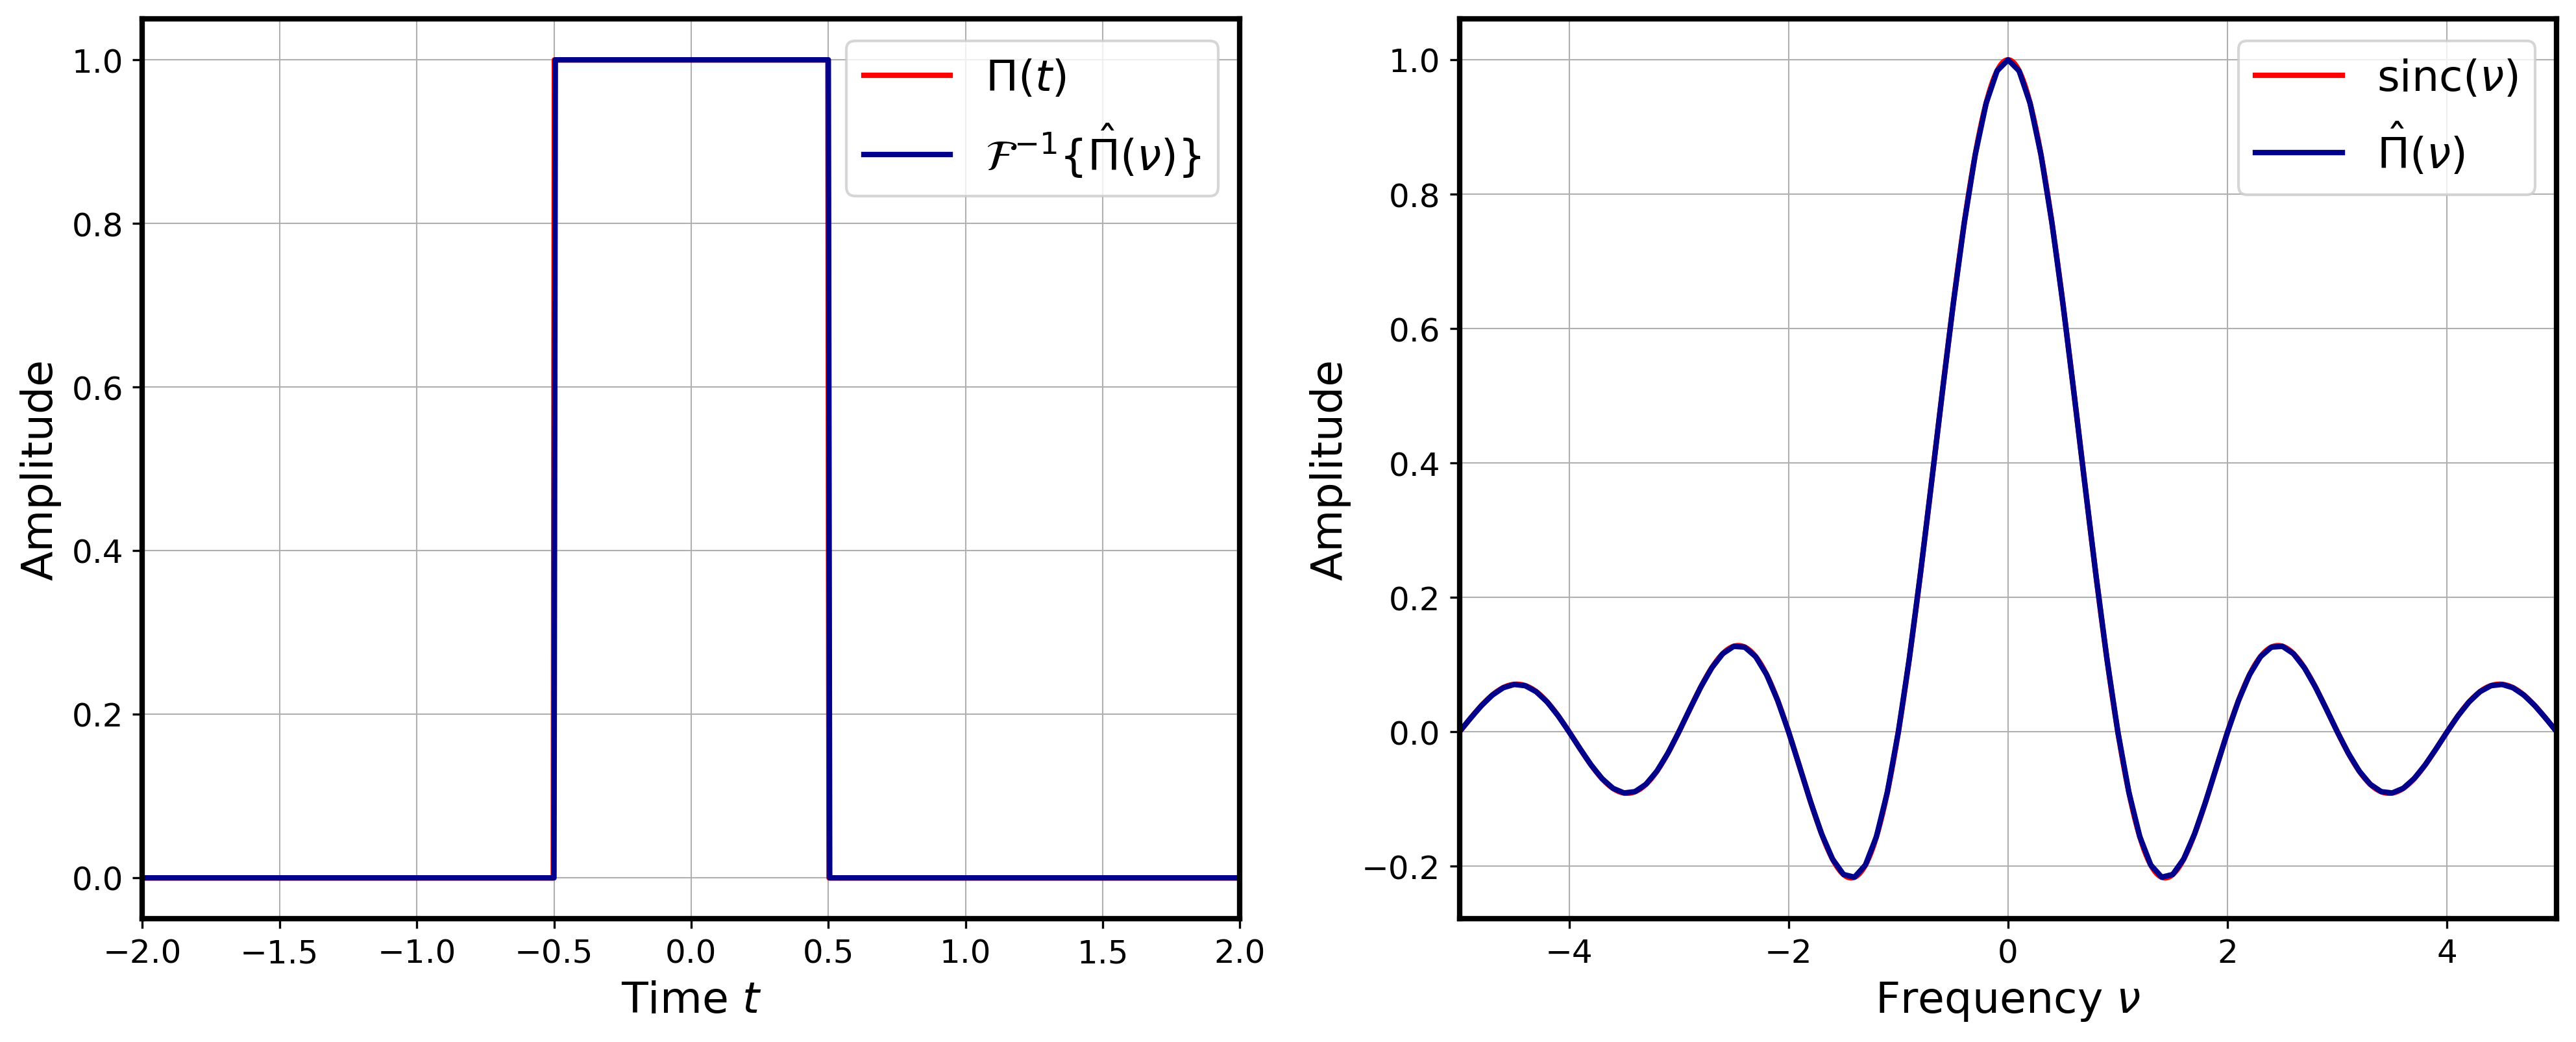
\includegraphics[width=1\textwidth]{../images/task3/continuous_T_10_dt_0.005.png} 
	\caption{Графики функций и фурье-образов. \(T = 10\).}
\end{figure}

Частота дискретизации \[\Delta \nu = \frac{1}{10} = 0.1\]


\begin{figure}[H]
	\centering
	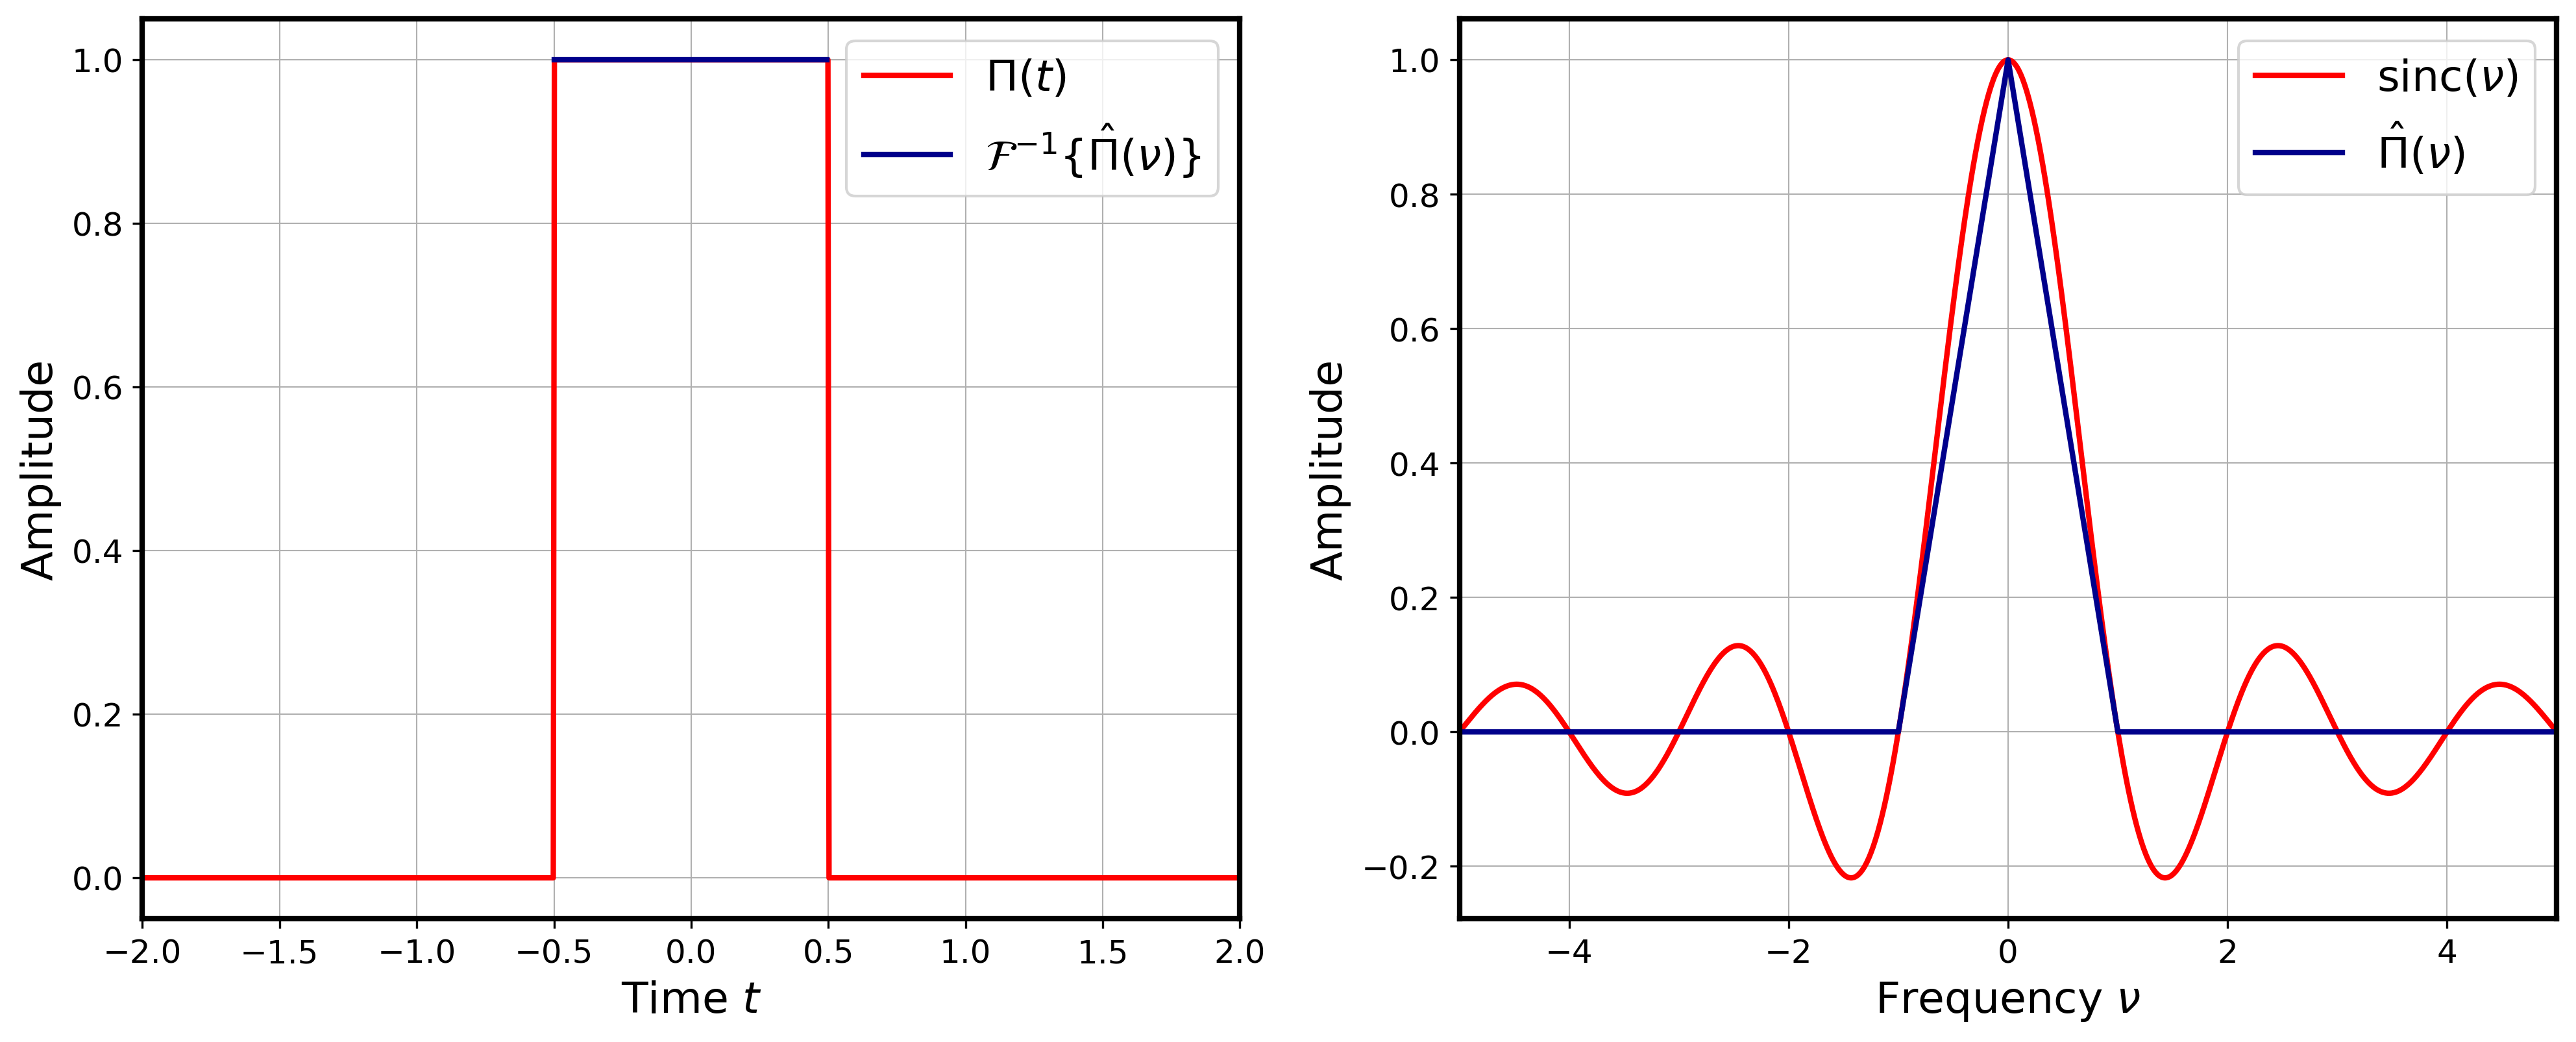
\includegraphics[width=1\textwidth]{../images/task3/continuous_T_1_dt_0.005.png} 
	\caption{Графики функций и фурье-образов. \(T = 1\).}
\end{figure}

Частота дискретизации \[\Delta \nu = \frac{1}{1} = 1\]

\subsubsection{Влияние параметра \(\Delta t\)}

Зафиксирую \(T = 20\). Возьму значения \(T \in [0.01, 0.1, 0.4]\) и посмотрю на изменения. Для каждого \(\Delta t\) расчитаю параметр длины частотного диапазона по формуле \[V = \frac{1}{\Delta t}\] А для фиксированного значения \(T = 20\) можно расчитать частоту дискретизации по формуле \[\Delta \nu = \frac{1}{T} = \frac{1}{20} = 0.05\]

\begin{figure}[H]
	\centering
	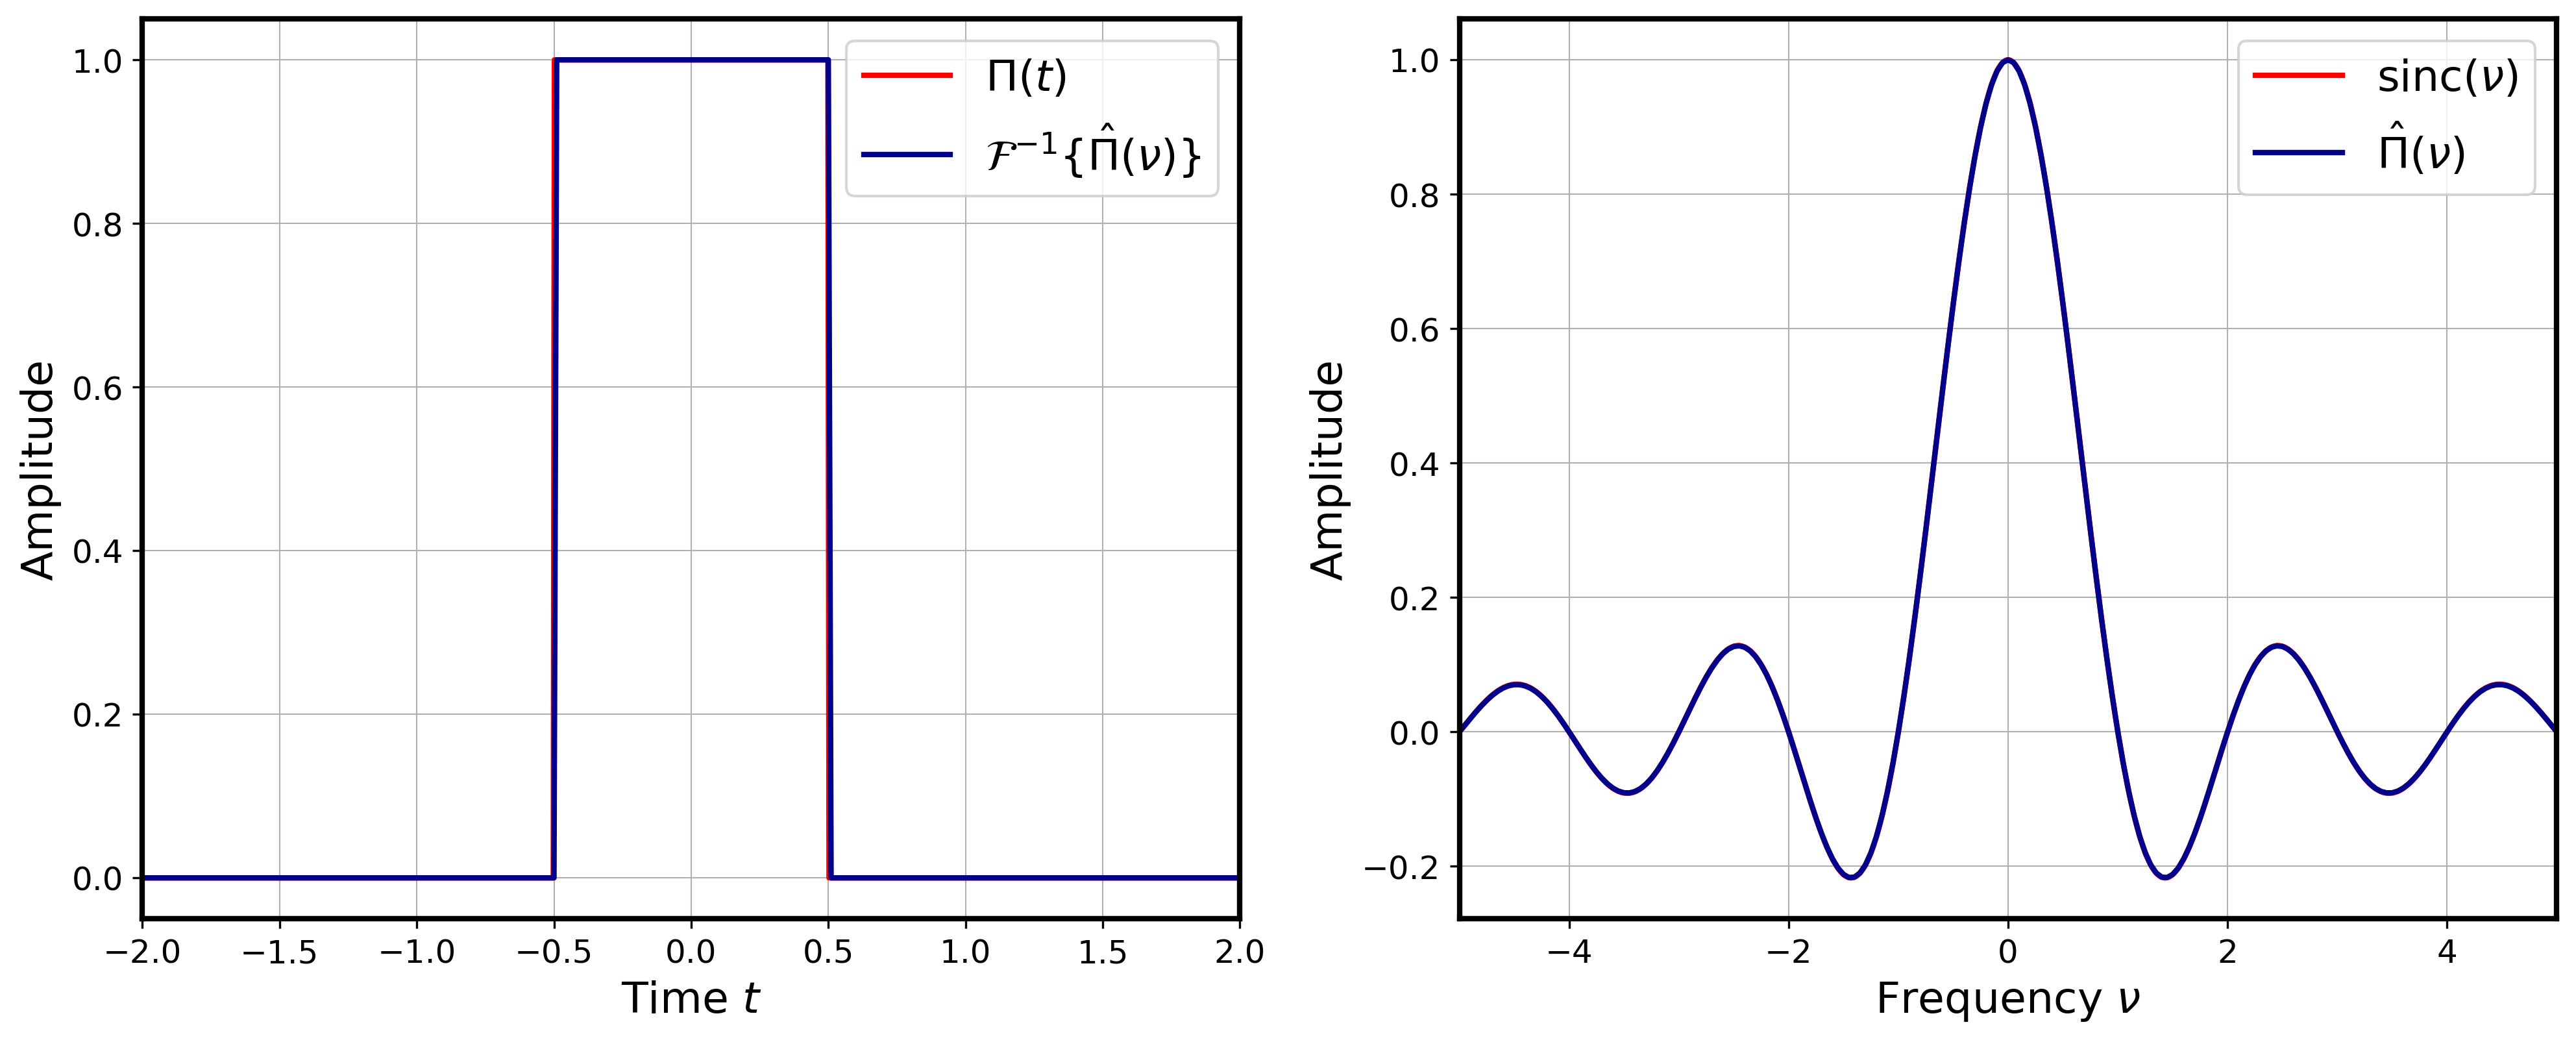
\includegraphics[width=1\textwidth]{../images/task3/continuous_T_20_dt_0.01.png} 
	\caption{Графики функций и фурье-образов. \(\Delta t = 0.01\).}
\end{figure}

Длина частотного диапазона \[V = \frac{1}{0.01} = 100\]

\begin{figure}[H]
	\centering
	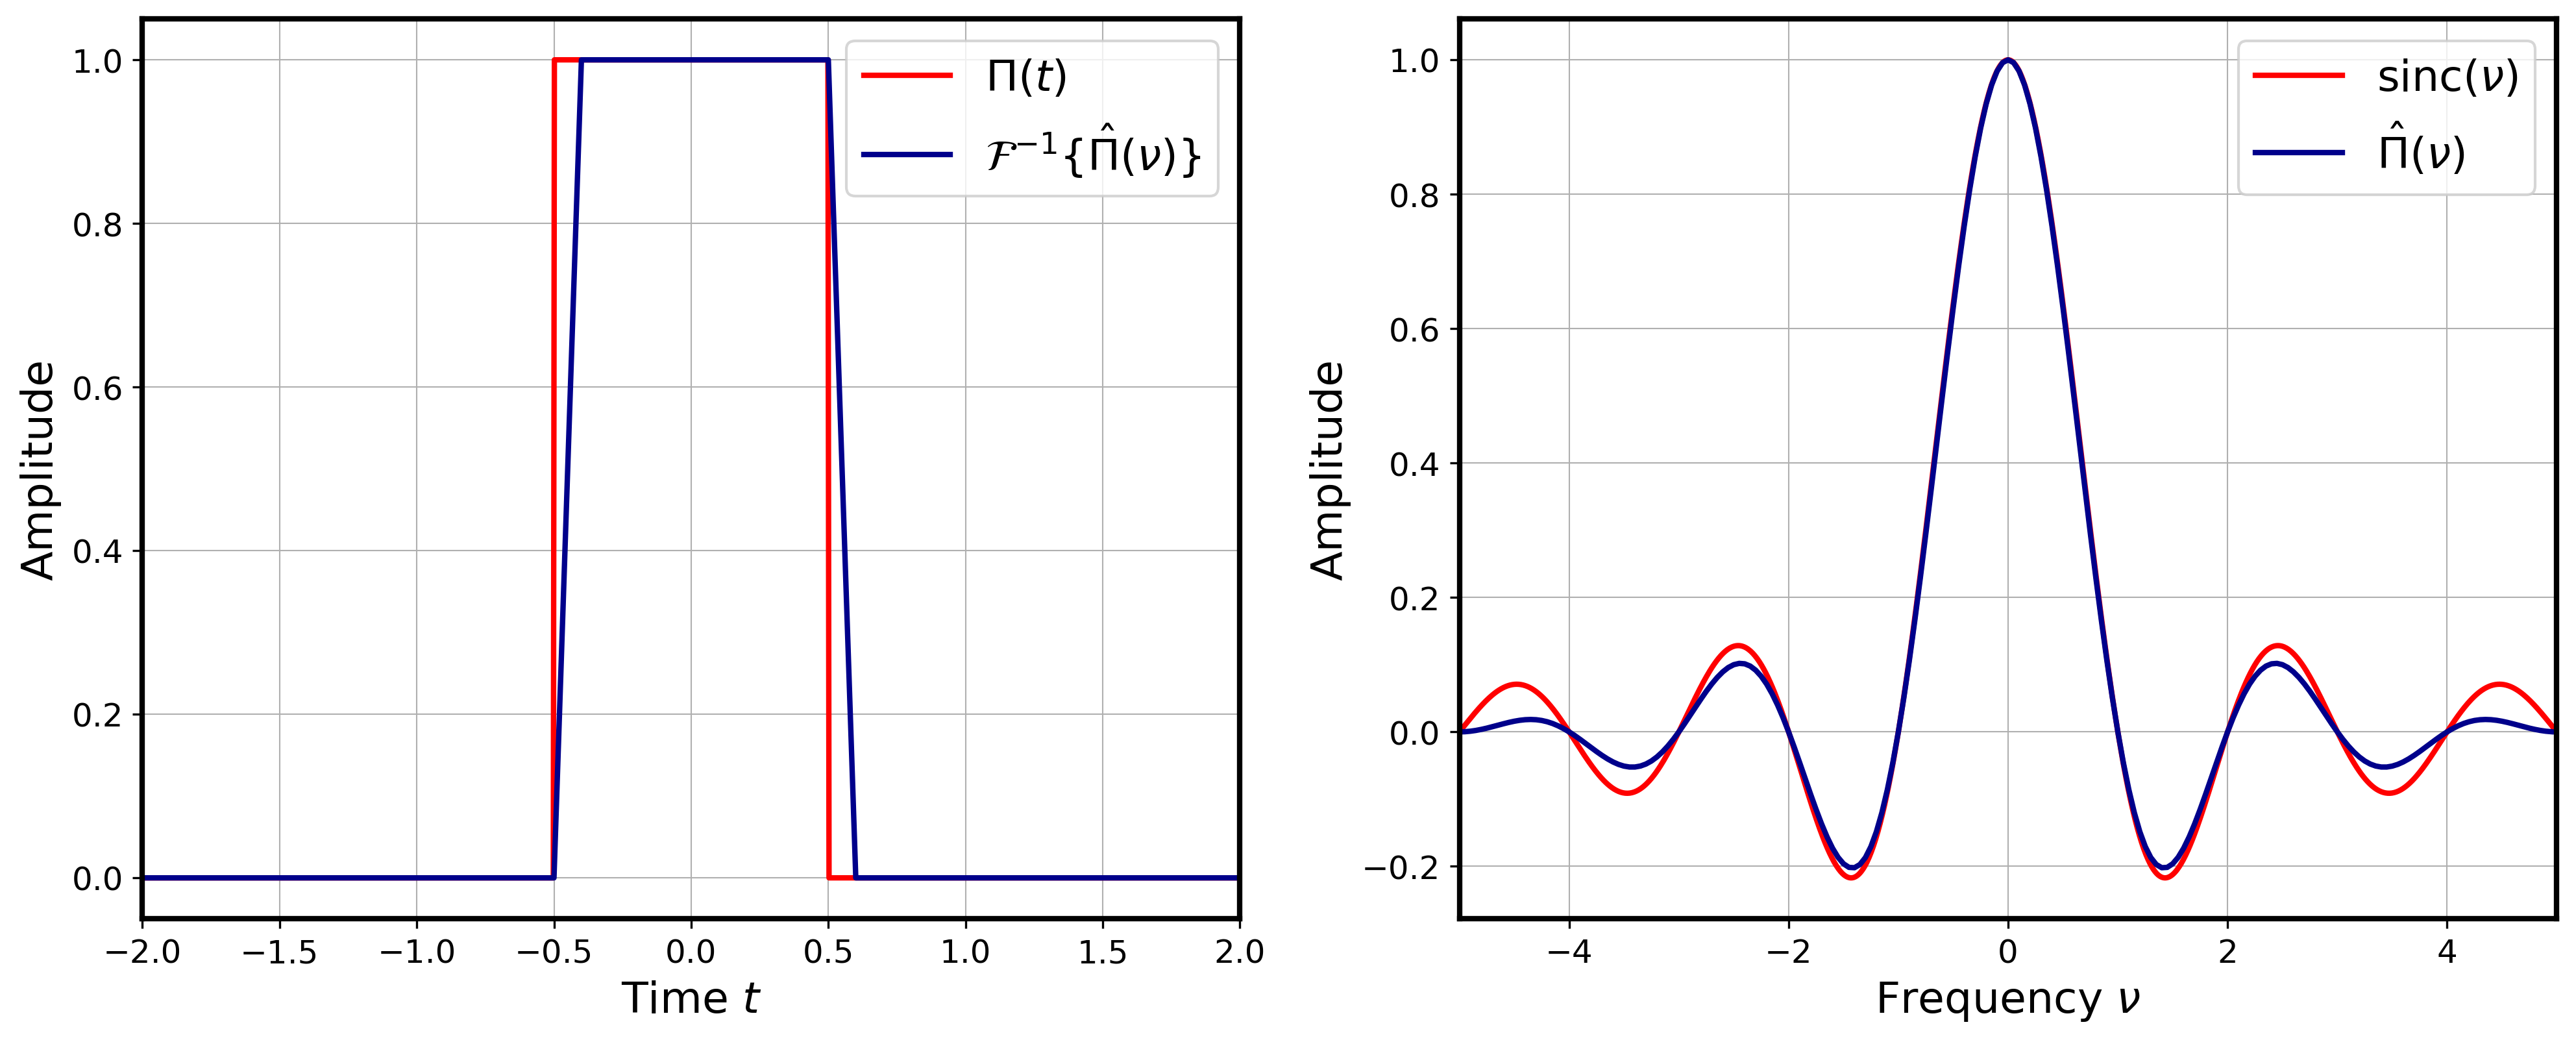
\includegraphics[width=1\textwidth]{../images/task3/continuous_T_20_dt_0.1.png} 
	\caption{Графики функций и фурье-образов. \(\Delta t = 0.1\).}
\end{figure}

Длина частотного диапазона \[V = \frac{1}{0.1} = 10\]


\begin{figure}[H]
	\centering
	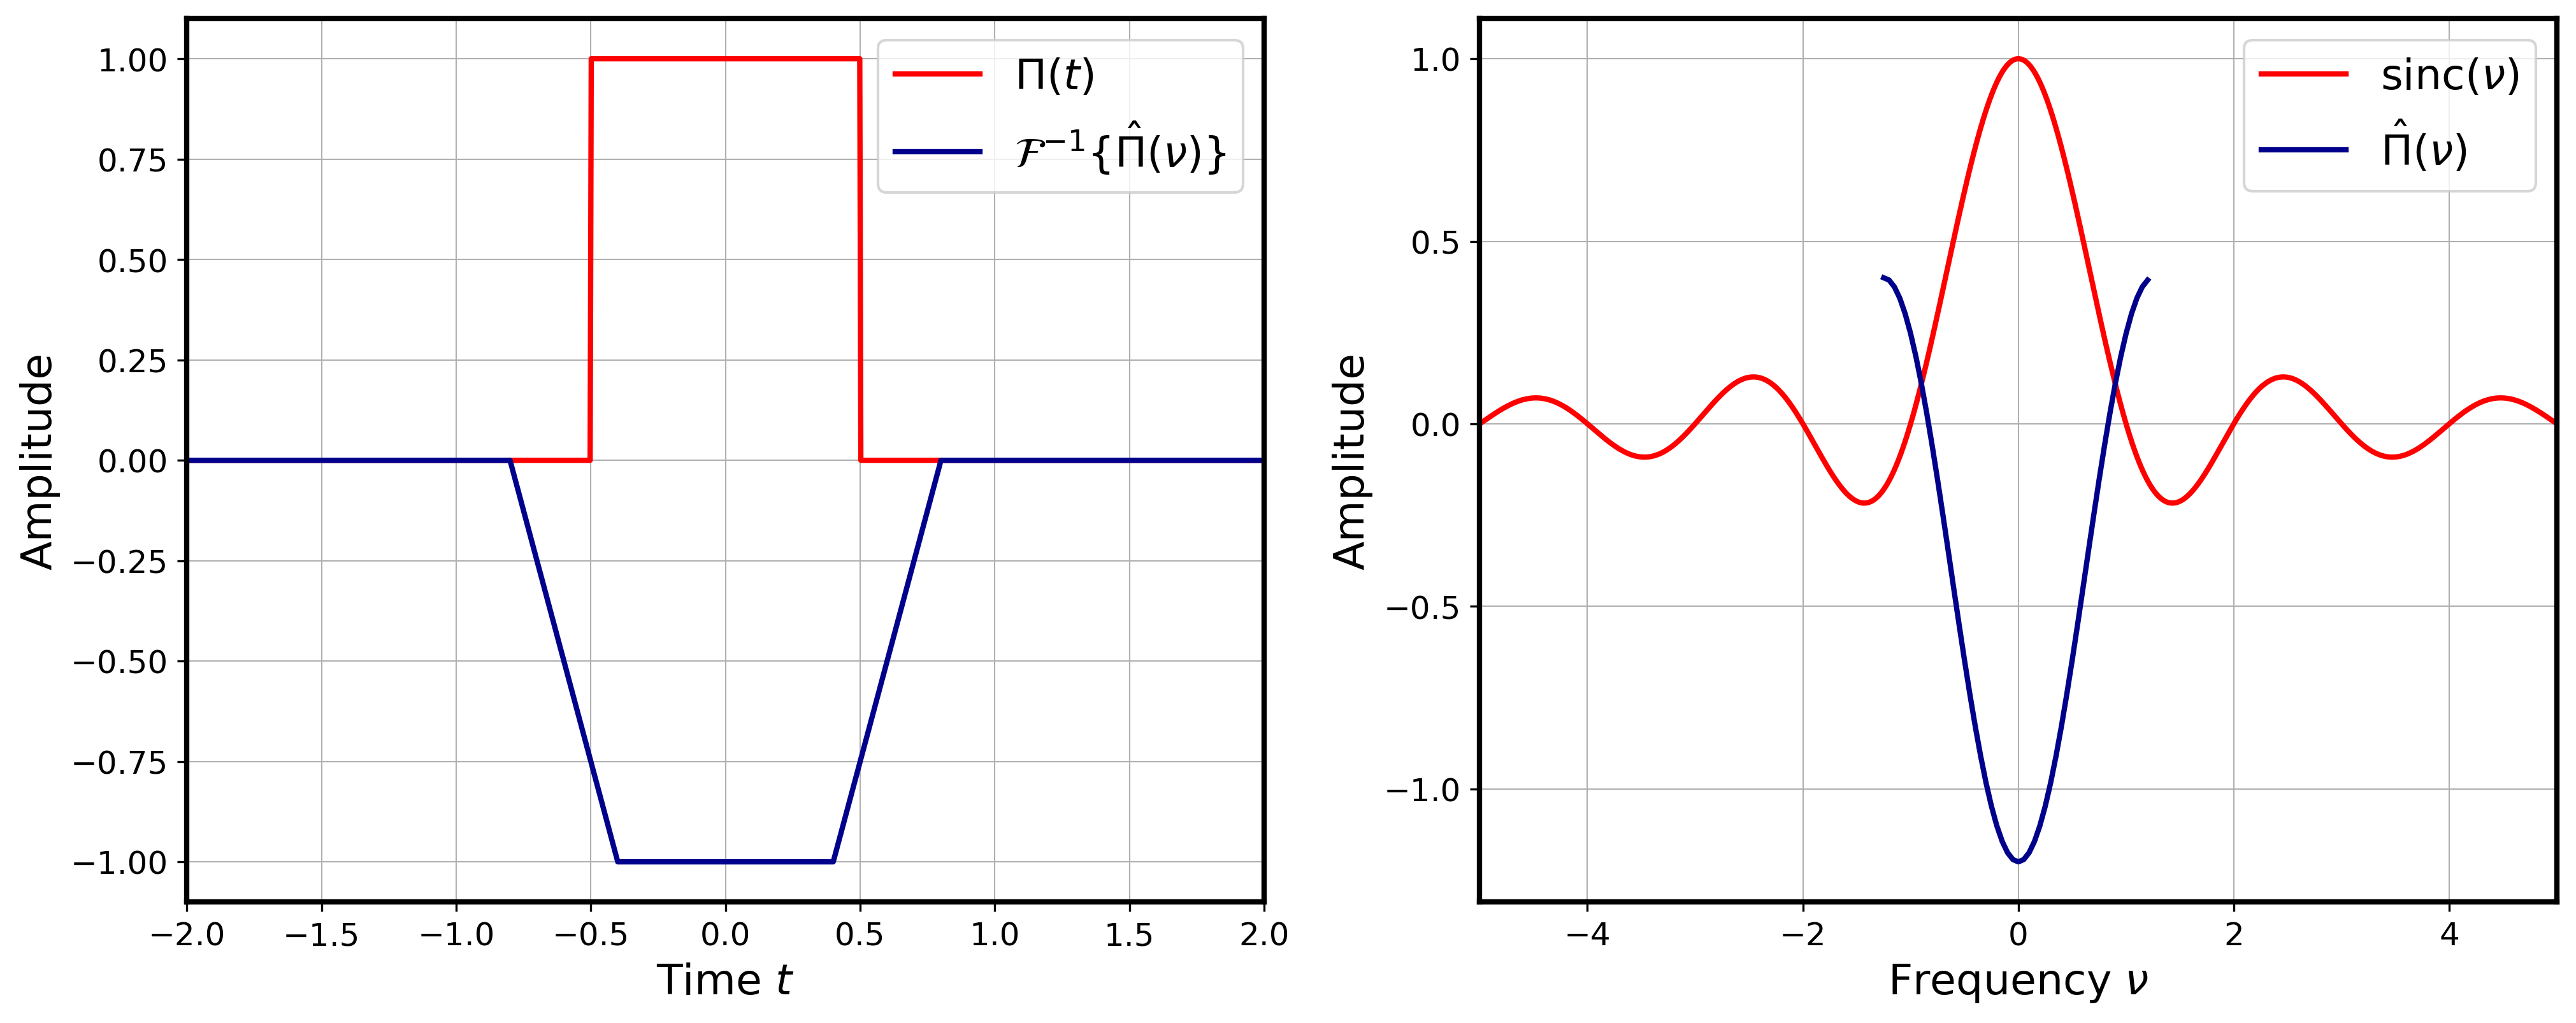
\includegraphics[width=1\textwidth]{../images/task3/continuous_T_20_dt_0.4.png} 
	\caption{Графики функций и фурье-образов. \(\Delta t = 0.4\).}
\end{figure}

Длина частотного диапазона \[V = \frac{1}{0.4} = 2.5\]

\subsubsection{Вывод}
Сигнул хорошо восстаналивается при всех выбранных параметрах \(T\), но чрезмерное уменьшение параметра \(\Delta t\) приводит к искажению сигнала и образа. Необходимо качественно подбирать коэффициенты.

\subsection{Сравнение трех методов}

Возьму наиболее показательные значения параметров $T = 40$, $\Delta t = 0.04$, $V = 40$, $\Delta \nu = 0.04$. Произведу сравнение трех методов на одном графике.

\begin{figure}[H]
	\centering
	
\includegraphics[width=1\textwidth]{../images/methods.png} 
	\caption{Графики функций и фурье-образов.}
\end{figure}

Для практических применений наиболее оптимальным является использование непрерывного преобразования Фурье с корректирующими коэффициентами, которое обеспечивает высокую точность при разумных вычислительных затратах. Численное интегрирование целесообразно использовать только в случаях, требующих максимальной точности без ограничений по времени вычислений.

\newpage

\section{Задание. Сэмплирование.}

В задании нужно сделать исследование теоремы Найквиста-Шеннона-Котельникова для функций:

\begin{align*}
y_1(t) &= a_1 \sin(\omega_1 t + \varphi_1) + a_2 \sin(\omega_2 t + \varphi_2) \\
y_2(t) &= \text{sinc}(bt)
\end{align*}


\textbf{Ожидаемые результаты}
\begin{itemize}
	\item Построить непрерывные графики функций
	\item Провести дискретизацию с шагом $\Delta t$
	\item Восстановить функции по формуле Котельникова
	\item Исследовать влияние шага дискретизации
	\item Найти спектры функций $\hat{y}_n(\nu)$
	\item Сравнить результаты с теоремой Найквиста
\end{itemize}

\textbf{Теорема Найквиста:} $\Delta t \leq \frac{1}{2B}$, где $B$ - максимальная частота

\subsection{Предподготовка}

Для этого задания выберу параметры:
\begin{align*}
a_1 &= 2.0, \quad a_2 = 1.5 \\
\omega_1 &= 3\pi, \quad \omega_2 = 8\pi \\
\varphi_1 &= \frac{\pi}{3}, \quad \varphi_2 = \frac{\pi}{4} \\
b &= 3\pi, \quad B = 6
\end{align*}

Тогда получатся функции
\begin{itemize}
	\item $y_1(t) = 2\sin(3\pi t + \frac{\pi}{3}) + 1.5\sin(8\pi t + \frac{\pi}{4})$
	\item $y_2(t) = \text{sinc}(3\pi t)$
\end{itemize}

Возьму параметры \(T = 50\), \(\Delta t = 0.005\). Чтобы соблюдалась теорема Найквиста значение \(\Delta t_{sample}\) должно быть \(\Delta t_{sample} \leq \frac{1}{12}\).

\subsection{Первая функция}

Построю график функции \[y_1(t) = 2\sin(3\pi t + \frac{\pi}{3}) + 1.5\sin(8\pi t + \frac{\pi}{4})\] без видимой дискретизации.

\begin{figure}[H]
	\centering
	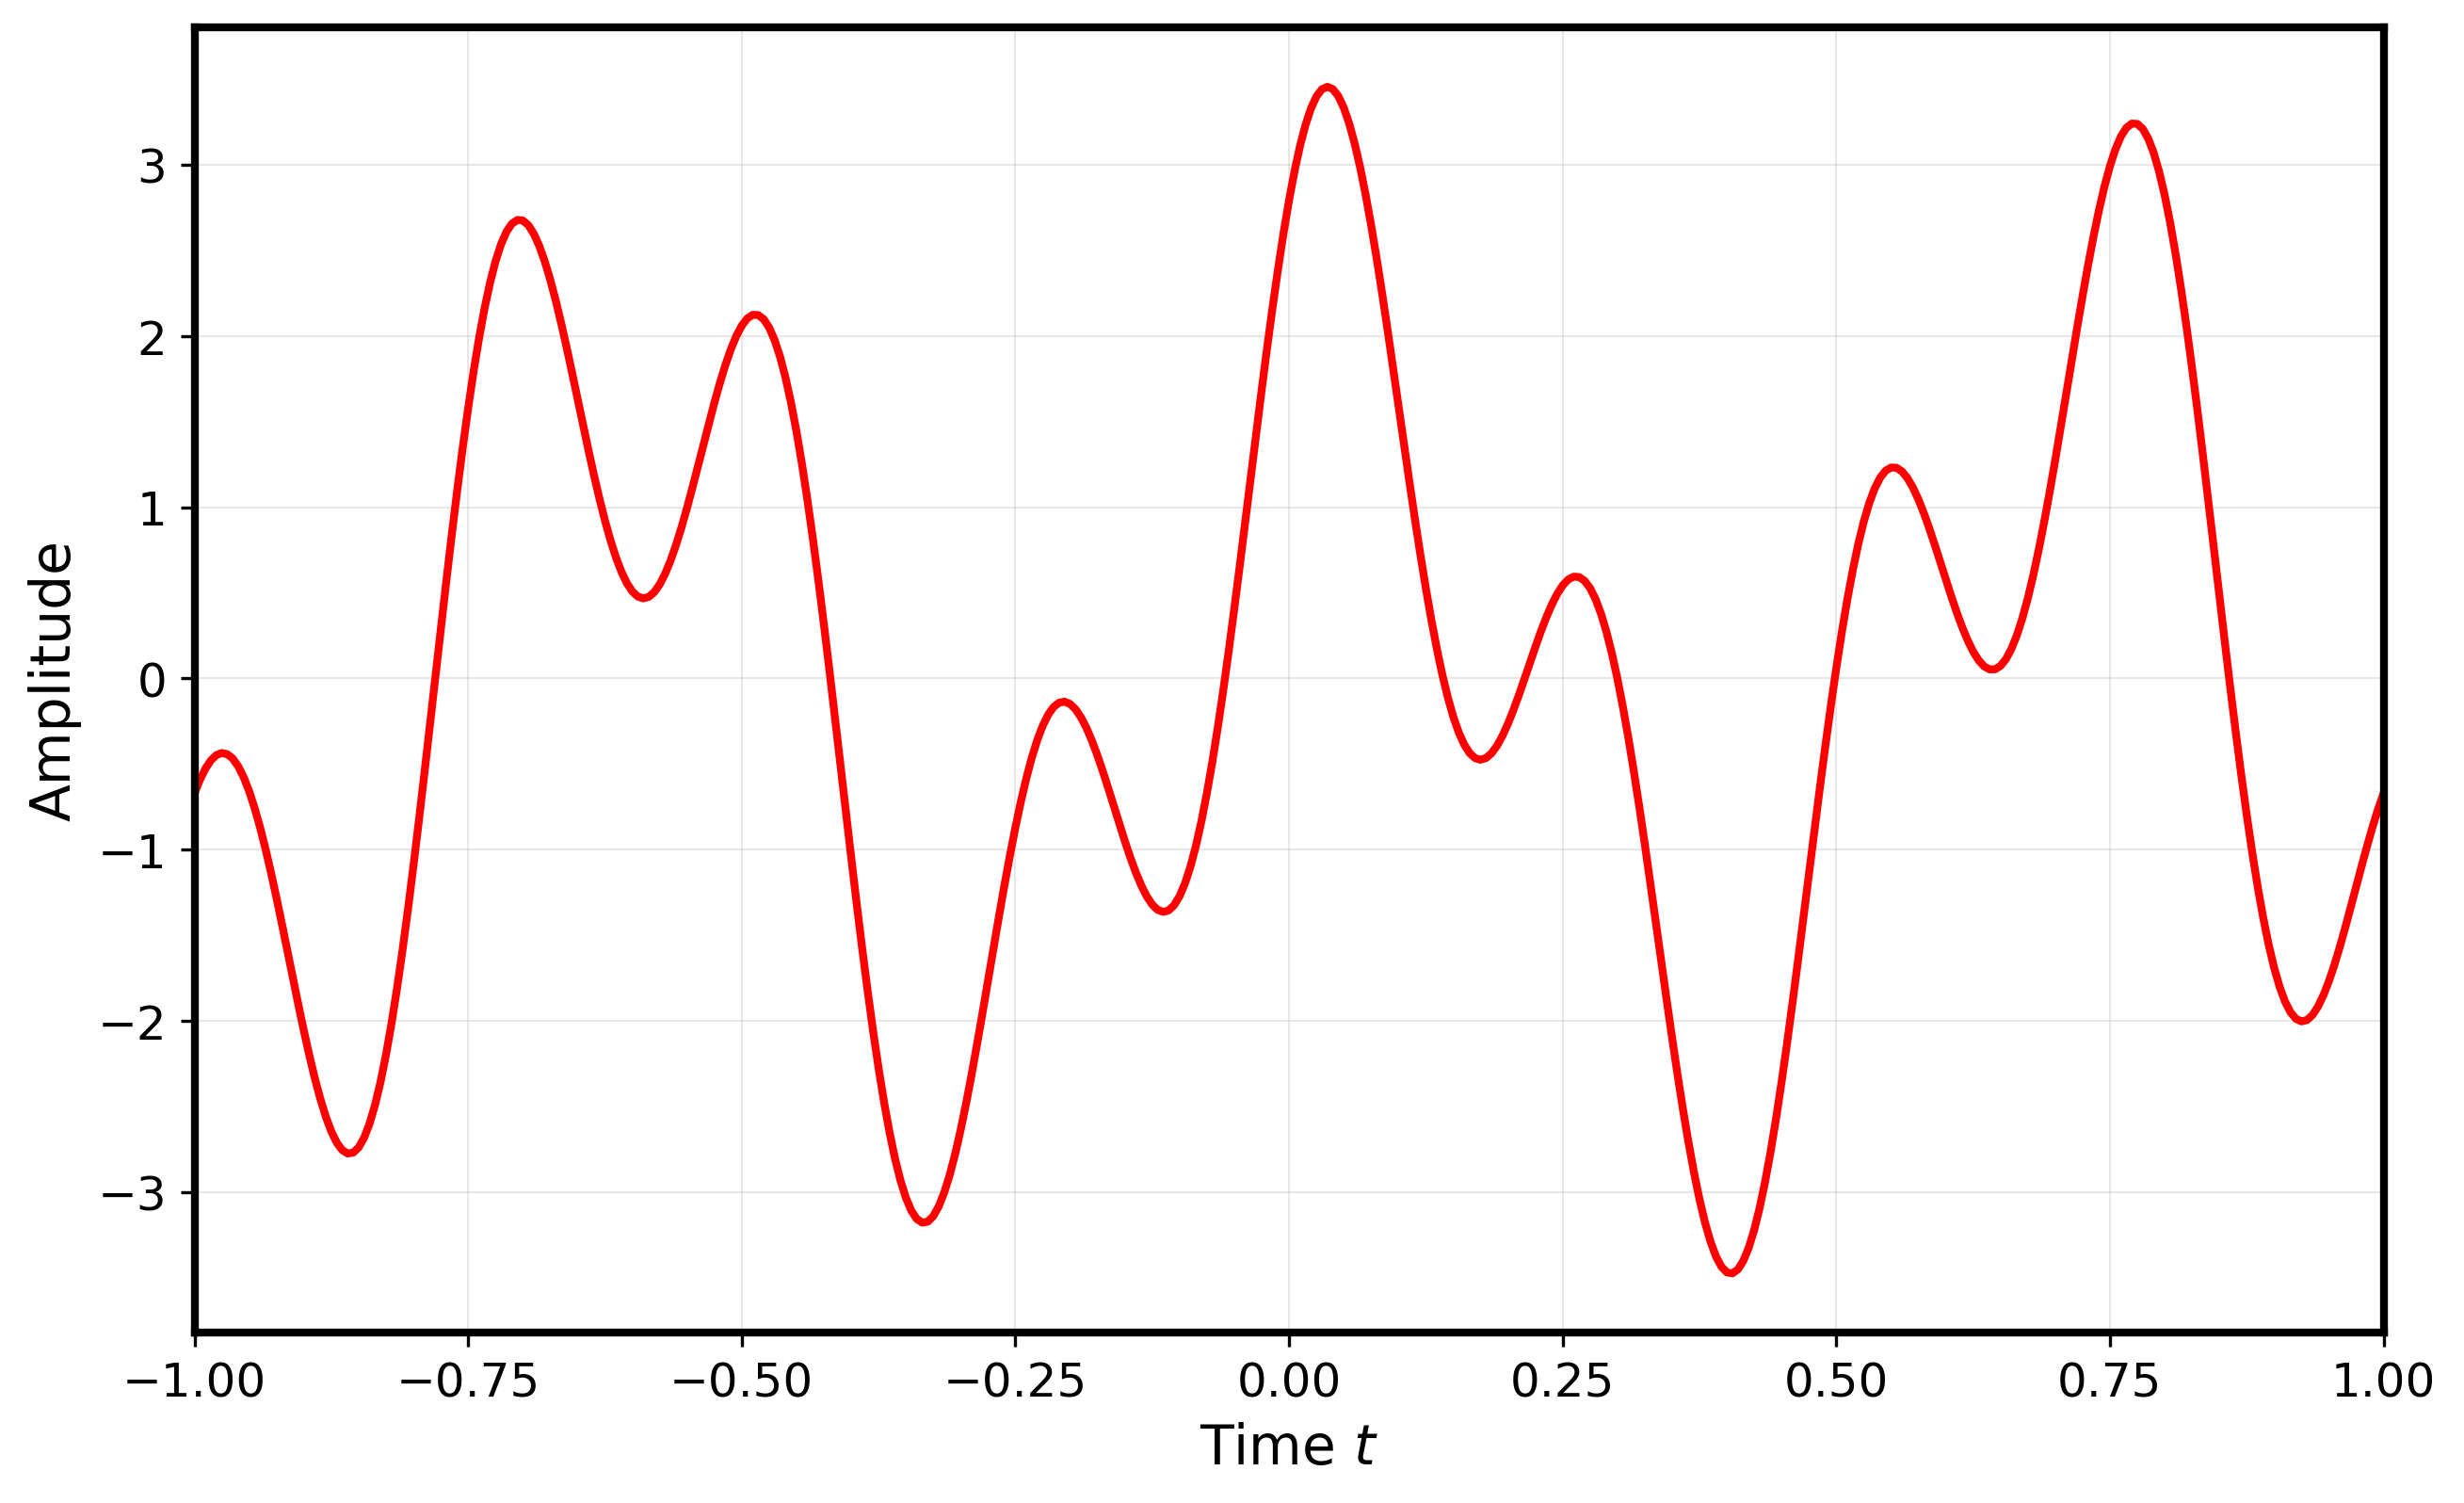
\includegraphics[width=0.8\textwidth]{../images/original_y1.png} 
	\caption{График функции \(y_1(t)\).}
\end{figure}

Возьму два значения \(\Delta t_{sample} \in [\frac{1}{5}, \frac{1}{100}]\). Первое удовлетворяет условию теоремы, а второе нет. 

\subsubsection{Нарушение условия теоремы}

При \(\Delta t_{sample} = \frac{1}{5}\) построю график исходной функции \(y_1(t)\) и сэмплированной.

\begin{figure}[H]
	\centering
	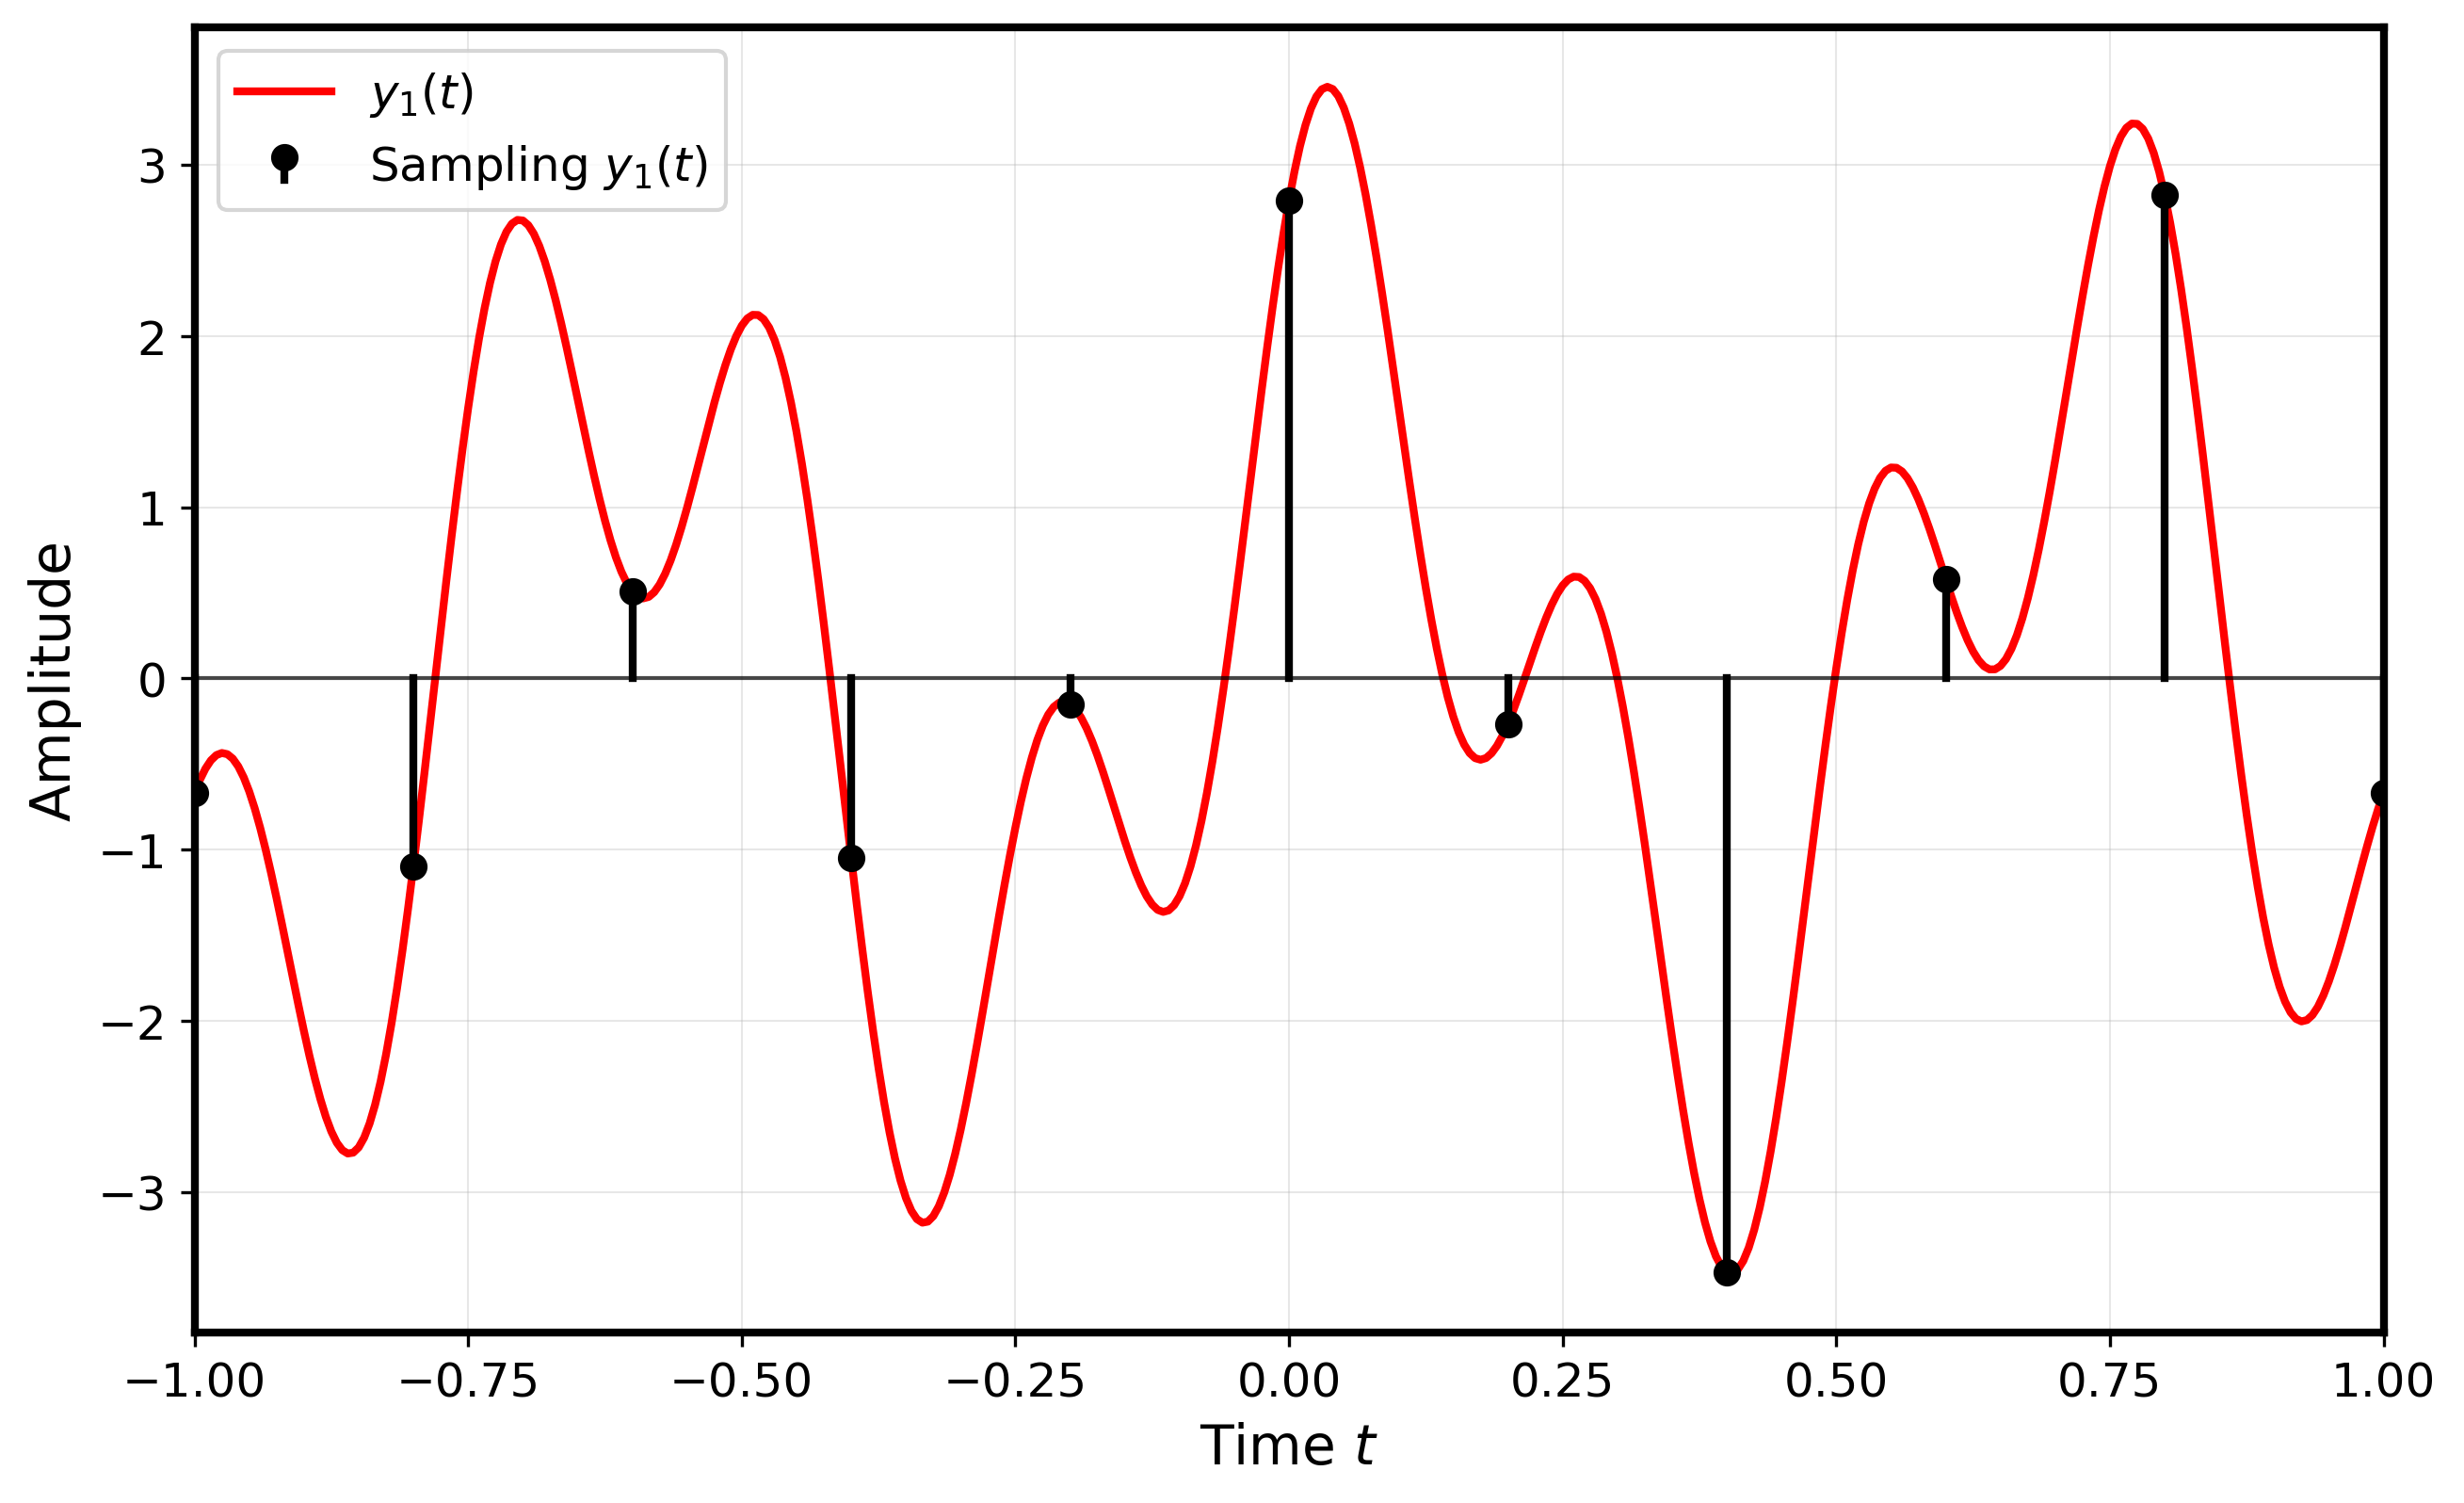
\includegraphics[width=0.8\textwidth]{../images/sampling_y1_violation.png} 
	\caption{График функций \(y_1(t)\) и сэмплированой.}
\end{figure}

Применю формулу интерполяции
\[
y_1(t) = \sum_{n=-B}^{B} y_1(t_n) \cdot \text{sinc}(2B(t - t_n))
\] к сэмплированному варианту функции:

\begin{figure}[H]
	\centering
	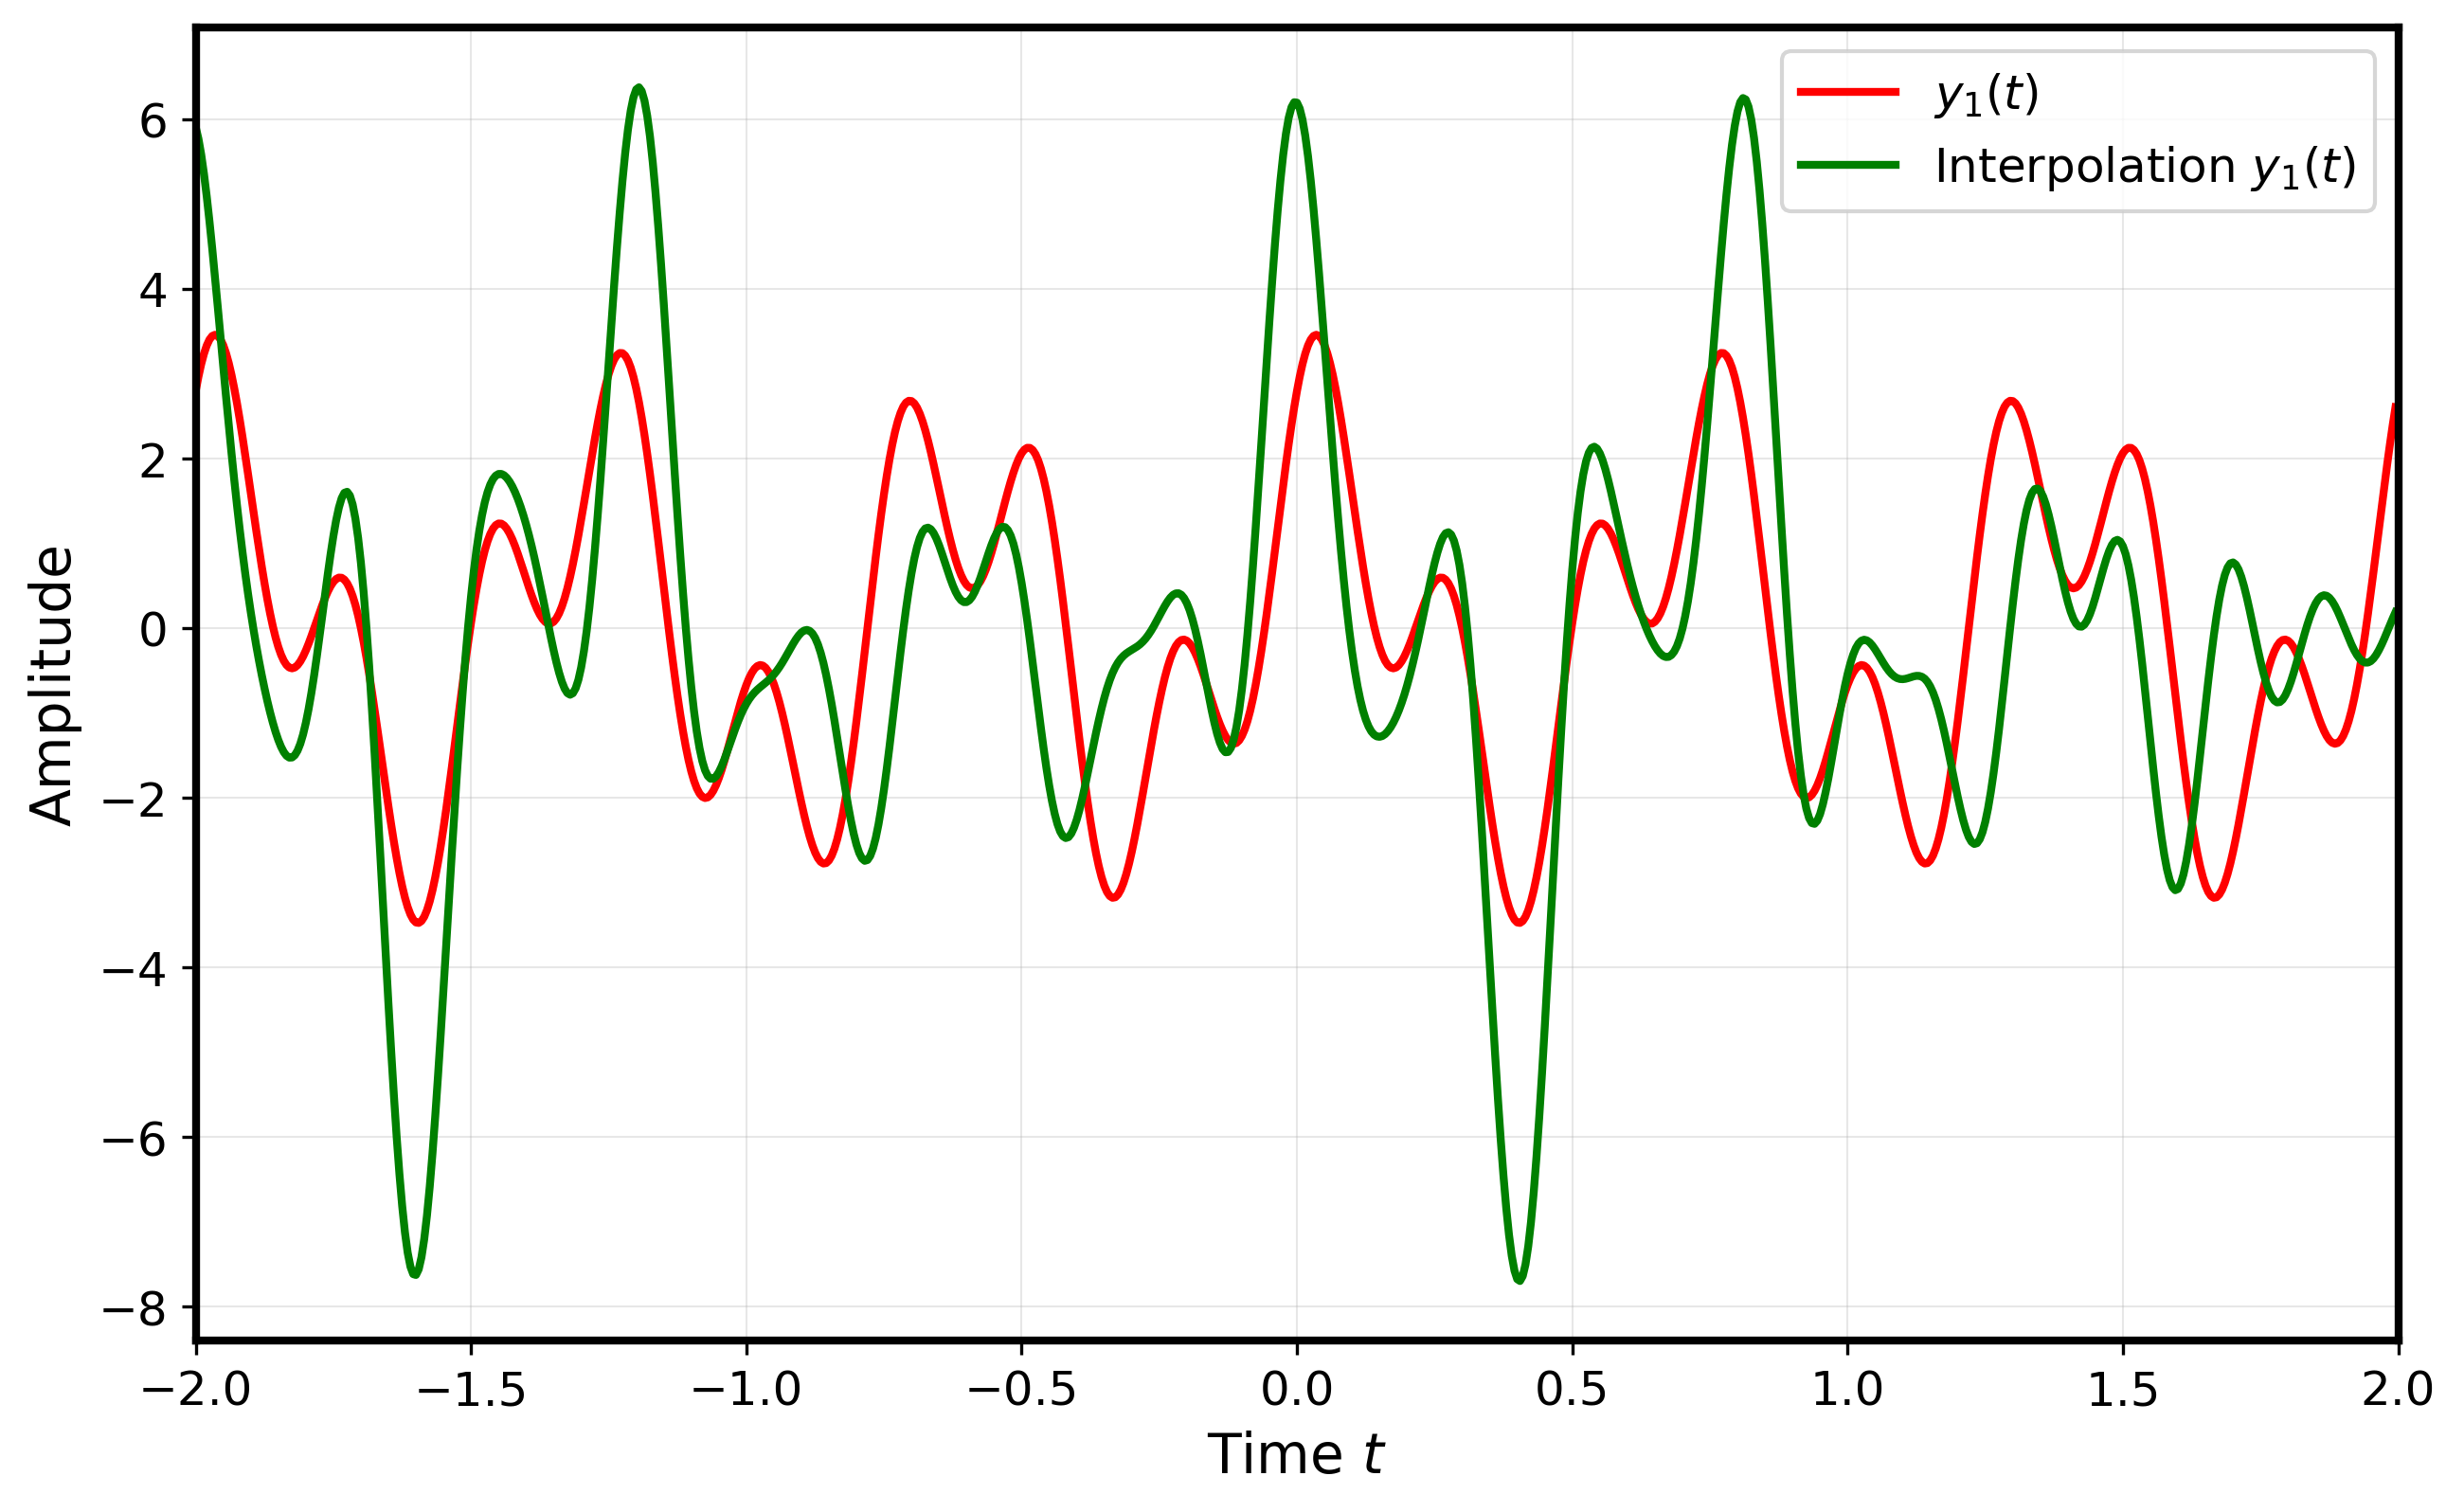
\includegraphics[width=0.8\textwidth]{../images/reconstruction_y1_violation.png} 
	\caption{График функций \(y_1(t)\) интерполяционной.}
\end{figure}

\subsubsection{Соблюдение условия теоремы}

При \(\Delta t_{sample} = \frac{1}{100}\) построю график исходной функции \(y_1(t)\) и сэмплированной.

\begin{figure}[H]
	\centering
	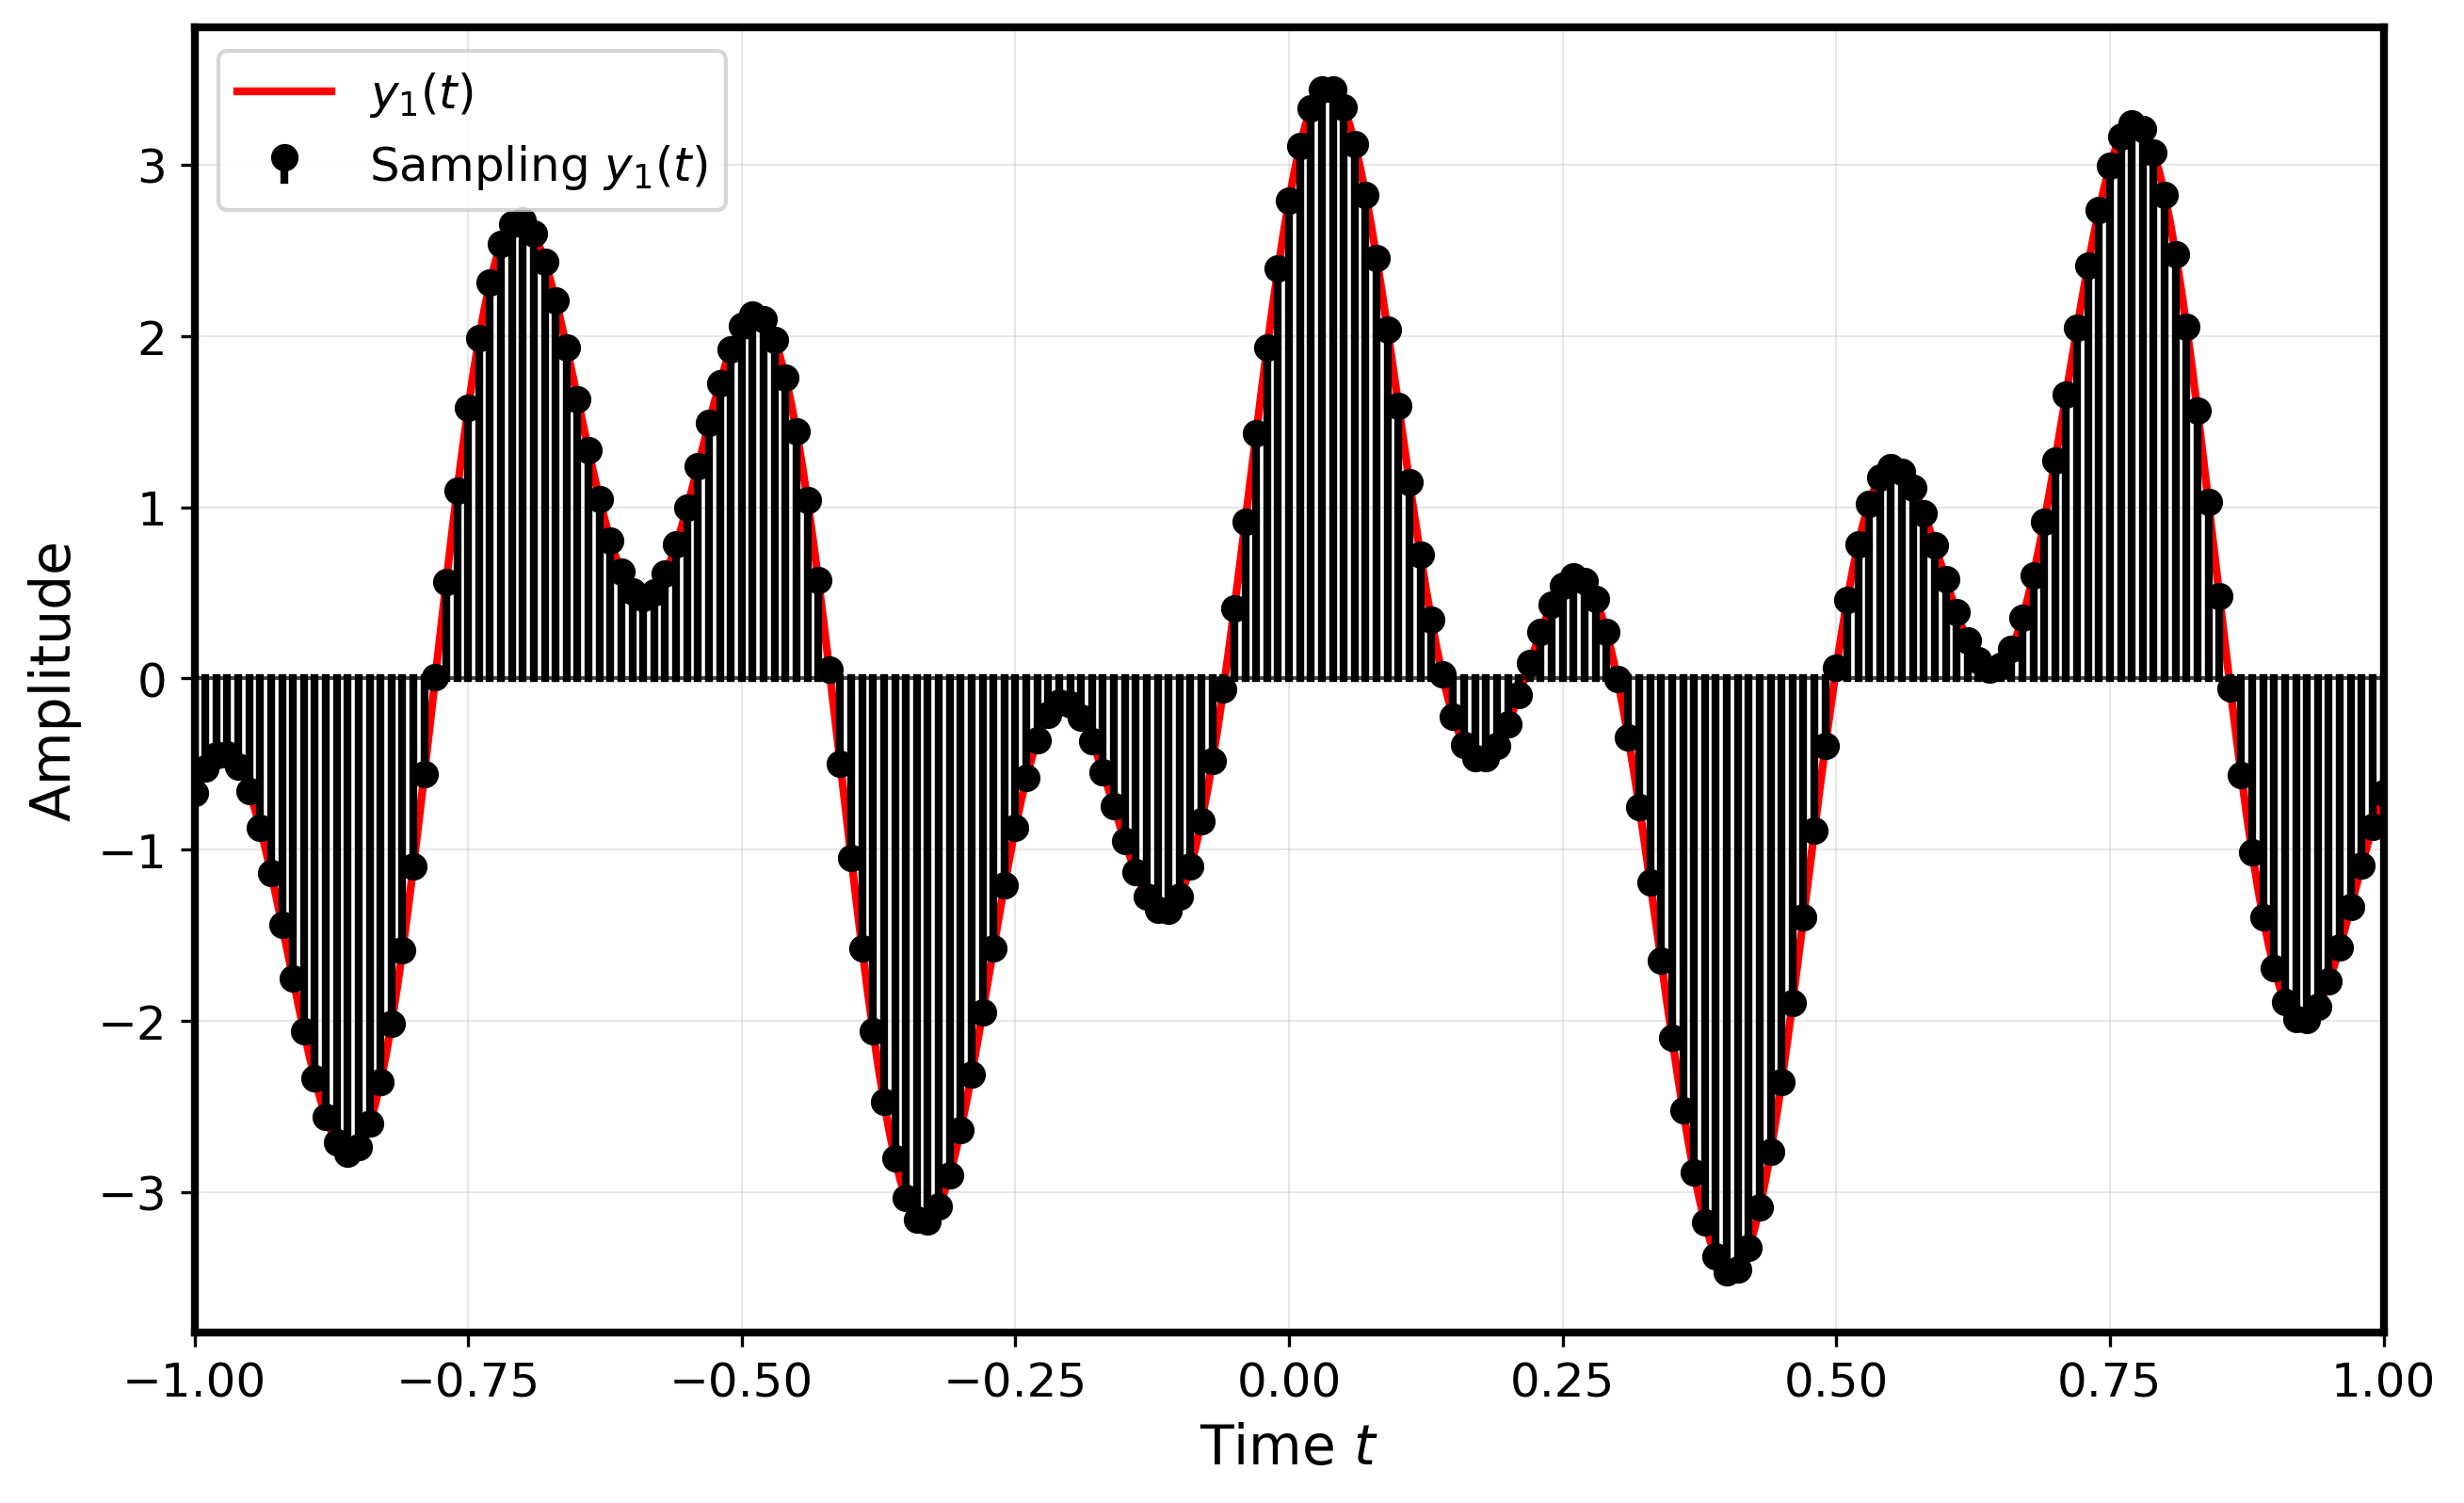
\includegraphics[width=0.8\textwidth]{../images/sampling_y1_nyquist.png} 
	\caption{График функций \(y_1(t)\) и сэмплированой.}
\end{figure}

Также построю график исходной и интерполяционной функции

\begin{figure}[H]
	\centering
	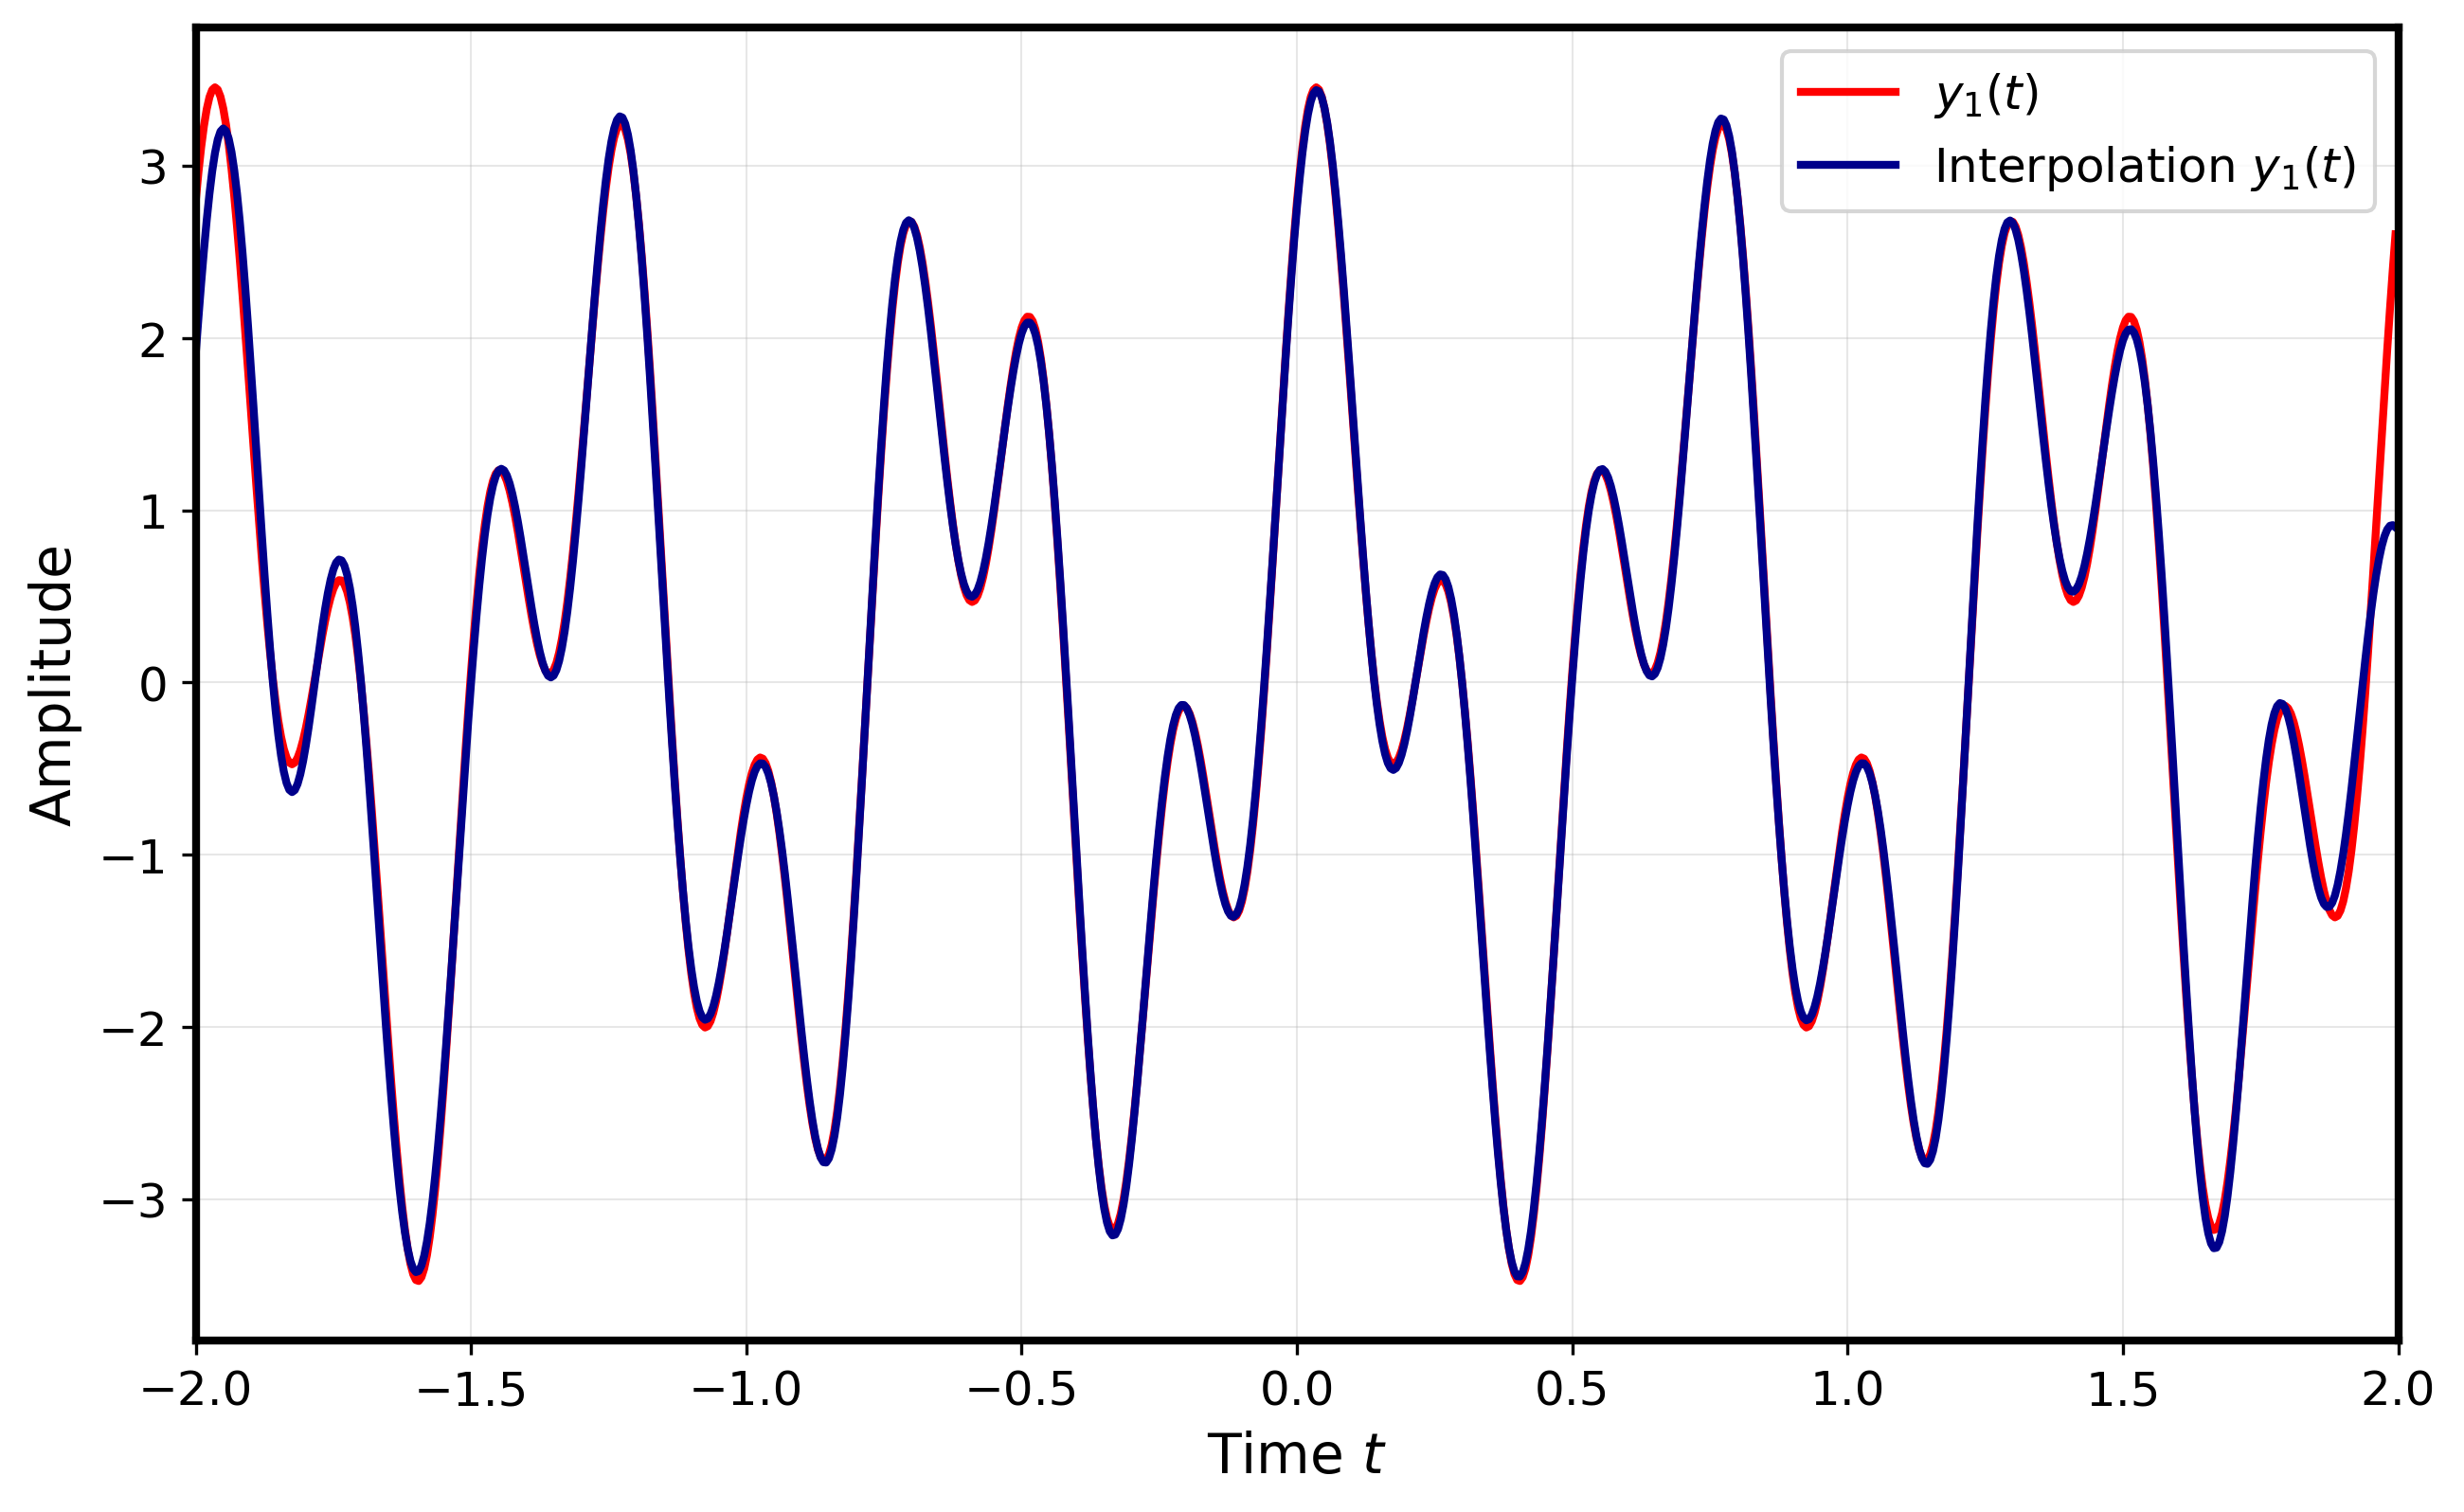
\includegraphics[width=0.8\textwidth]{../images/reconstruction_y1_nyquist.png} 
	\caption{График функций \(y_1(t)\) интерполяционной.}
\end{figure}

\subsubsection{Сравнение фурье-образов}

\end{document}

	
	